% This must be in the first 5 lines to tell arXiv to use pdfLaTeX, which is strongly recommended.
\pdfoutput=1
% In particular, the hyperref package requires pdfLaTeX in order to break URLs across lines.

\documentclass[twocolumn]{article}

% Change "review" to "final" to generate the final (sometimes called camera-ready) version.
% Change to "preprint" to generate a non-anonymous version with page numbers.
\usepackage[preprint]{acl}

% Standard package includes
\usepackage{times}
\usepackage{pdfpages}
\usepackage{latexsym}
\usepackage{array}
\usepackage{lipsum}  
\usepackage{makecell}
\usepackage{booktabs}
\usepackage{graphicx}
\usepackage{caption}
\usepackage{booktabs}
\usepackage{xcolor}
\usepackage{enumitem}
% \usepackage[margin=1in]{geometry}
\usepackage{array}
\usepackage{longtable}
\usepackage{natbib} 
\usepackage{standalone}
\usepackage{subcaption}
\usepackage{tikz}
\usepackage{pgfplots}
\pgfplotsset{compat=1.18}
\usepackage{array}
\usepackage[ruled,vlined]{algorithm2e}
\usepackage{colortbl}  % For row colors
\usepackage{array}     % For better table formatting
\usepackage{amsmath}
\usepackage{booktabs}  % For better table formatting
% For proper rendering and hyphenation of words containing Latin characters (including in bib files)
\usepackage[T1]{fontenc}
\SetCommentSty{textit}  % Make comments italic
\SetVlineSkip{0.5em}   % Adjust vertical line spacing
% For Vietnamese characters
% \usepackage[T5]{fontenc}
% See https://www.latex-project.org/help/documentation/encguide.pdf for other character sets

% This assumes your files are encoded as UTF8
\usepackage[utf8]{inputenc}

% This is not strictly necessary, and may be commented out,
% but it will improve the layout of the manuscript,
% and will typically save some space.
\usepackage{microtype}

% This is also not strictly necessary, and may be commented out.
% However, it will improve the aesthetics of text in
% the typewriter font.
\usepackage{inconsolata}

%Including images in your LaTeX document requires adding
%additional package(s)
\usepackage{graphicx}
% \usepackage{algorithm}
% \usepackage{algorithmic}
\usepackage{algpseudocode}
\usepackage{multirow}
\usepackage{tabularx}   % For tables with adjustable-width columns
\usepackage{amsmath}
\usepackage[utf8]{inputenc}
\usepackage{verbatim} % or use the listings package if preferred
\usepackage{amsthm}
\usepackage{amssymb}
\usepackage{pifont}
\usepackage{fontawesome}
% \usepackage{bbding}
% \usepackage{tcolorbox}
% \usepackage{xcolor}
% \usepackage{fontawesome}

% Optional: If you want to customize the algorithm appearance
\renewcommand{\algorithmicrequire}{\textbf{Input:}}
\renewcommand{\algorithmicensure}{\textbf{Output:}}
\setlength{\parskip}{0.5em} % Or whatever value you prefer
% If the title and author information does not fit in the area allocated, uncomment the following
%
%\setlength\titlebox{<dim>}
%
% and set <dim> to something 5cm or larger.


\title{MedHallu: A Comprehensive Benchmark for Detecting Medical Hallucinations in Large Language Models}

% Author information can be set in various styles:
% For several authors from the same institution:
% \author{Author 1 \and ... \and Author n \\
%         Address line \\ ... \\ Address line}
% if the names do not fit well on one line use
%         Author 1 \\ {\bf Author 2} \\ ... \\ {\bf Author n} \\
% For authors from different institutions:
% \author{Author 1 \\ Address line \\  ... \\ Address line
%         \And  ... \And
%         Author n \\ Address line \\ ... \\ Address line}
% To start a separate ``row'' of authors use \AND, as in
% \author{Author 1 \\ Address line \\  ... \\ Address line
%         \AND
%         Author 2 \\ Address line \\ ... \\ Address line \And
%         Author 3 \\ Address line \\ ... \\ Address line}

% \author{First Author \\
%   Affiliation / Address line 1 \\
%   Affiliation / Address line 2 \\
%   Affiliation / Address line 3 \\
%   \texttt{email@domain} \\\And
%   Second Author \\
%   Affiliation / Address line 1 \\
%   Affiliation / Address line 2 \\
%   Affiliation / Address line 3 \\
%   \texttt{email@domain} \\}

\author{
 \textbf{Shrey Pandit\textsuperscript{1}\thanks{Corresponding author: \href{mailto:shreypandit@utexas.edu}{shreypandit@utexas.edu}}},
 \textbf{Jiawei Xu\textsuperscript{1}},
 \textbf{Junyuan Hong\textsuperscript{1}},\\
 \textbf{Zhangyang Wang\textsuperscript{1}},
 \textbf{Tianlong Chen\textsuperscript{2}},
 \textbf{Kaidi Xu\textsuperscript{3}},
 \textbf{Ying Ding\textsuperscript{1}}
% \\
%  \textbf{Fifth Author\textsuperscript{1,2}},
%  \textbf{Sixth Author\textsuperscript{1}},
%  \textbf{Seventh Author\textsuperscript{1}},
%  \textbf{Eighth Author \textsuperscript{1,2,3,4}},
%\\
%  \textbf{Ninth Author\textsuperscript{1}},
%  \textbf{Tenth Author\textsuperscript{1}},
%  \textbf{Eleventh E. Author\textsuperscript{1,2,3,4,5}},
%  \textbf{Twelfth Author\textsuperscript{1}},
%\\
%  \textbf{Thirteenth Author\textsuperscript{3}},
%  \textbf{Fourteenth F. Author\textsuperscript{2,4}},
%  \textbf{Fifteenth Author\textsuperscript{1}},
%  \textbf{Sixteenth Author\textsuperscript{1}},
%\\
%  \textbf{Seventeenth S. Author\textsuperscript{4,5}},
%  \textbf{Eighteenth Author\textsuperscript{3,4}},
%  \textbf{Nineteenth N. Author\textsuperscript{2,5}},
%  \textbf{Twentieth Author\textsuperscript{1}}
\\
\faGlobe~Dataset \& Code: \url{https://medhallu.github.io/} \\
 \textsuperscript{1}University of Texas at Austin,
 \textsuperscript{2}UNC Chapel Hill,
 \textsuperscript{3}Drexel University,
 % \textsuperscript{4}Affiliation 4,
 % \textsuperscript{5}Affiliation 5
% \\
 % \small{
 %      Data and Code: \href{https://medhallu.github.io/}{https://medhallu.github.io/}
 % }
}


\begin{document}
\maketitle
\begin{abstract}
Advancements in Large Language Models (LLMs) and their increasing use in medical question-answering necessitate rigorous evaluation of their reliability. A critical challenge lies in hallucination, where models generate plausible yet factually incorrect outputs. In the medical domain, this poses serious risks to patient safety and clinical decision-making. To address this, we introduce \textbf{MedHallu}, the first benchmark specifically designed for medical hallucination detection. MedHallu comprises 10,000 high-quality question-answer pairs derived from PubMedQA, with hallucinated answers systematically generated through a controlled pipeline. Our experiments show that state-of-the-art LLMs, including GPT-4o, Llama-3.1, and the medically fine-tuned UltraMedical, struggle with this binary hallucination detection task, with the best model achieving an F1 score as low as 0.625 for detecting ``hard'' category hallucinations. Using bidirectional entailment clustering, we show that harder-to-detect hallucinations are semantically closer to ground truth. Through experiments, we also show incorporating domain-specific knowledge and introducing a ``not sure'' category as one of the answer categories improves the precision and F1 scores by up to 38\% relative to baselines. 
% The MedHallu benchmark is publicly accessible at [LINK].
\end{abstract}

\section{Introduction}
Recent advances in Large Language Models (LLMs)~\citep{achiam2023gpt} have catalyzed their widespread adoption as assistive tools across a multitude of domains, including software development~\citep{Krishna_2024_software}, healthcare ~\citep{singhal2022largelanguagemodelsencode_health}, weather prediction~\citep{li2024cllmatemultimodalllmweather}, and financial applications \citep{nie2024surveylargelanguagemodels}. However, LLMs are prone to hallucination~\citep{bang2023multitaskmultilingualmultimodalevaluation_hallucination}, where they generate plausible but factually incorrect or unverifiable information~\citep{Ji_2023_12RW, Huang_2025_survey11}. Hallucinations can arise from various factors, including biased or insufficient training data~\citep{han2024skipnsimplemethod_data, zhang2024knowledgeovershadowingcausesamalgamated_data}, and inherent architectural limitations of LLMs \citep{leng2023mitigatingobjecthallucinationslarge_architecture, kalai2024calibratedlanguagemodelshallucinate_architecture}. This issue is particularly problematic in high-stakes fields such as the medical domains, where the generation of incorrect information can exacerbate health disparities~\citep{singhal2022largelanguagemodelsencode_health}. 

 % Efforts to address hallucination involve implementing strategies such as Retrieval-Augmented Generation \citep{Semnani_2023_RAG_Hallu}, self-refinement techniques \citep{huang2022largelanguagemodelsselfimprove} \citep{wang2023selfconsistencyimproveschainthought}, and rigorous fine-tuning on factual datasets. These approaches aim to enhance the reliability of AI outputs in healthcare settings. Nonetheless, challenges remain in ensuring the scalability and generalizability of these strategies, highlighting the need for ongoing research and development in the field.

\begin{figure}[t]
\centering
\includegraphics[width=1\linewidth]{figures/figure_1.pdf}
\caption{An example of medical hallucination detection. The detailed prompt used for the hallucination detection task is presented in Appendix \ref{appendix:prompt}.}
\label{fig:task}
\end{figure}

Detecting hallucinations in LLM outputs (Figure~\ref{fig:task}) is therefore of critical importance. Various methods have been proposed to address this issue, including self-consistency~\citep{wang2023selfconsistencyimproveschainthought}, sampling-based approaches such as SelfCheckGPTZero \citep{manakul2023selfcheckgptzeroresourceblackboxhallucination_detect1}, and intrinsic methods that evaluate token-level uncertainty and entropy~\citep{azaria2023internalstatellmknows_detect2, xiao2021hallucinationpredictiveuncertaintyconditional_detect3}.
Existing benchmarks, such as HaluEval~\citep{Hallueval} and Haydes~\citep{liu2022tokenlevelreferencefreehallucinationdetection} primarily evaluate hallucination detection capabilities on general tasks, including summarization, question answering, and dialogue systems, with an emphasis on common-sense knowledge rather than domain specificity. 
% \kaidi{the following paragraph is very important, please use \ding{202} \ding{203} \ding{204} to oragnize them}  
This gap becomes particularly consequential in the medical domains, where specialized terminology requires precise handling, as minor lexical deviations can lead to substantially divergent interpretations~\citep{singhal2022largelanguagemodelsencode_health}. While recent efforts such as HaluBench~\citep{ravi2024lynxopensourcehallucination}, incorporate limited samples from the medical domains, their domain-agnostic generation frameworks lack medical curation. Similarly, Med-Halt~\citep{pal2023medhaltmedicaldomainhallucination} focuses on model benchmarking rather than providing a structured evaluation resource. Furthermore, the subtlety of hallucinations (e.g., whether they are hard or easy to detect) remains underexplored in the medical context. Additionally, the performance differences between pre-trained LLMs and fine-tuned medical LLMs are sparsely documented~\cite{ravi2024lynxopensourcehallucination, Hallueval, pal2023medhaltmedicaldomainhallucination}.

To address these gaps, we present the \textbf{Med}ical \textbf{Hallu}cination detection dataset (\textbf{MedHallu}), a comprehensive corpus of 10,000 medical question-answer pairs derived from the established PubMedQA dataset. Each pair is meticulously annotated to distinguish accurate responses from hallucinated content. Furthermore, MedHallu is stratified into easy, medium, and hard detection tiers based on the subtlety of hallucinations, enabling granular evaluation of model capabilities. The primary contributions of this research are threefold:
 \begin{itemize}
 \vspace{-3mm}
     \item We introduce MedHallu, one of the first datasets specifically designed for medical hallucination detection tasks. Comprising 10,000 entries derived from PubMedQA, MedHallu is systematically categorized into three levels of difficulty—easy, medium, and hard—based on the subtlety of hallucination detection.

     \item We find that hallucinated answers that are semantically closer to the ground truth are more challenging to detect. Furthermore, clustered answers using bi-directional entailment reveal uniformity, where all entries in a cluster are consistently either easy or hard to detect.

    \item Our evaluation shows that general-purpose LLMs outperform fine-tuned medical LLMs in medical hallucination detection tasks. Additionally, we find that model performance can be enhanced by providing relevant knowledge to LLMs. Moreover, introducing a ``not sure'' class alongside the existing classes of ``hallucinated'' and ``not-hallucinated'' leads to improved precision, which is critical in the medical domains.

 \end{itemize}

% \shreyp{WRITE SOMETHING ABOUT PAST WORK AND RESEARCH GAP}
% We further analyze the similarity between the hallucinated and ground truth samples by clustering the hallucinated answers using the bidirectional entailment method~\citep{Farquhar2024DetectingHI_semantic_entropy}. We find that hallucinated points that are harder to distinguish are semantically closer to the ground truth in metrics such as Euclidean distance, higher cosine similarity score, and high Rouge-2 score than those that are easy to detect, giving insights on LLMs discriminatory behavior, pointing to that it is the semantic meaning of a sentence that is resulting in difficult detection rather than syntactic behavior. 

% Previous works such as HaluBench \citep{ravi2024lynxopensourcehallucination}, HaluEval \cite{Hallueval}, and Med-HALT \citep{pal2023medhaltmedicaldomainhallucination} have primarily focused on examining general-purpose LLMs for their ability to detect hallucinations. These studies have not examined how domain-specific Large Language Models perform in these tasks. To address this gap, we assess fine-tuned medical LLMs, mainly Med42-8B \citep{med42v2}, Meditron3-8B, OpenBioLLM-8B \citep{OpenBioLLMs} and UltraMedical-8B \citep{zhang2024ultramedical} in the context of medical hallucination detection task as described in figure \ref{fig:task}, and discover that their performance is inferior to that of their instruction-tuned counterparts. Our methodology for dataset creation is detailed in Section \ref{Methodology}.


 
\begin{figure*}[ht]
\centering
\includegraphics[width=1\linewidth]{figures/figure_2.pdf}
\caption{\textbf{MedHallu} medical hallucinated answer generation pipeline. Each question-answer pair from the PubMedQA dataset undergoes the following steps to generate a hallucinated answer: (1) \textbf{Candidate Generation}: Given a question, relevant knowledge, and ground truth answer, the LLM is prompted to generate a hallucinated answer adhering to one of four hallucination types. (2) \textbf{Grading \& Filtering}: Generated answers undergo \textbf{quality} and \textbf{correctness} checks, being labeled as \textbf{hard}, \textbf{medium}, \textbf{easy}, or \textbf{failed} based on filtering results. (3) \textbf{Refining Failed Generation}: Failed answers are optimized using TextGrad~\cite{yuksekgonul2024textgradautomaticdifferentiationtext} and re-filtered. If they fail again, the LLM is re-prompted to generate new answers (\textbf{Regeneration}). (4) \textbf{Fallback}: If no qualified answers emerge after four regeneration attempts, the answer most similar to the ground truth is selected as an easy hallucinated example. The detailed prompt used for hallucination generation task is presented in the Appendix~\ref{appendix:prompt}.}
\label{fig:pipeline}
\end{figure*}

 % \begin{table}[h]
    \centering
    \small
    \renewcommand{\arraystretch}{1.2}  % Increases row spacing
    \begin{tabular}{|>{\raggedright\arraybackslash}p{0.1\textwidth}|>{\raggedright\arraybackslash}p{0.3\textwidth}|}
        \hline
        \rowcolor{gray!10} \textbf{Component} & \textbf{Content} \\
        \hline
        \textit{Question} & Is halofantrine ototoxic? \\
        \hline
        \textit{Ground Truth} & Halofantrine has mild to moderate pathological effects on cochlea histology, can be considered ototoxic drug. \\
        \hline
        \textit{Hallucinated Answer} & Halofantrine exhibits no ototoxicity and is generally considered safe for auditory function. \\
        \hline
    \end{tabular}
    \caption{An example in the MedHallu dataset.}
    \label{tab:dataset-example}
\end{table}
\vspace{-3mm}
\section{Related Work}
\vspace{-2mm}
\paragraph{Hallucination Detection Benchmarks.}
 Hallucination in LLMs has been extensively documented in a variety of tasks, including machine translation~\citep{lee2019hallucinations_13RW}, dialogue systems~\citep{balakrishnan-etal-2019-constrained_14RW}, text summarization~\citep{durmus-etal-2020-feqa_15RW}, and question answering~\citep{sellam2020bleurtlearningrobustmetrics_16RW}, as reviewed in recent surveys~\citep{Ji_2023_12RW}. Existing benchmarks for hallucination detection, such as Hades~\citep{liu2022tokenlevelreferencefreehallucinationdetection} and HaluEval~\citep{Hallueval}, offer robust methodologies for identifying hallucinated content. However, they predominantly employ generic techniques that fail to account for the nuanced complexities inherent in medical contexts. Similarly, while benchmarks such as HaluBench~\citep{ravi2024lynxopensourcehallucination} include some medical data samples in their data set, their data generation processes are not specifically tailored for the medical domain. Although Med-HALT~\citep{pal2023medhaltmedicaldomainhallucination} focuses on medical hallucinations, it mainly serves as a performance evaluation tool rather than providing a structured dataset. In contrast, our work introduces the first comprehensive dataset for medical hallucination detection, employing controlled methods to address these domain-specific challenges.
\vspace{-2mm}
\paragraph{Semantic Analysis of Hallucinated Text.}
Hallucinated sentences often sound over-confident~\citep{miao2021preventlanguagemodeloverconfident_overconfident, chen2022improvingfaithfulnessabstractivesummarization_overconfident} and frequently contain tokens that are statistically improbable within a given context, primarily due to suboptimal decoding strategies. Fine-tuned models have sought to mitigate this issue by adjusting decoding parameters to enhance factual accuracy, thereby reducing the occurrence of rare or anomalous terms in hallucinated outputs~\citep{Huang_2025_survey11}. Despite these advancements, previous research has not systematically compared hallucinated sentences with their corresponding ground truth to assess semantic similarities. Our work fills this gap by uncovering deeper semantic relationships between hallucinated texts and their ground truth counterparts.
\vspace{-2mm}

\paragraph{Improvement Methods in Hallucination Detection.}

Recent advancements in hallucination detection have focused on integrating external knowledge to enhance model performance. Retrieval-augmented methods~\citep{lewis2021retrievalaugmentedgenerationknowledgeintensivenlp_241, li2023weboysterimprovinglarge_242} have mitigate hallucinations via grounding models in general knowledge. However, few studies have examined the impact of domain-specific knowledge on hallucination detection tasks. While HaluEval~\citep{Hallueval} evaluates knowledge-augmented detection, it lacks fine-grained, domain-relevant knowledge integration. LLMs often overestimate their competence \citep{zhang2023sirenssongaiocean_247}, which underscores the need for structured mechanisms to allow models to abstain from answering when uncertain. Prior works have leveraged reinforcement learning~\cite{xu2024rejectionimprovesreliabilitytraining_246}, conformal abstention~\citep{yadkori2024mitigatingllmhallucinationsconformal_245}, or likelihood score and entropy-based metrics~\citep{cole2023selectivelyansweringambiguousquestions_248} to guide refusal decisions. However, these methods rely on complex supervision or predefined thresholds. More straightforward approaches, such as refusing to answer out-of-domain questions~\citep{cao2024learnrefusemakinglarge_244}, offer greater practicality but lack adaptability to domain-specific tasks, particularly in complex fields like medicine. Our work addresses these limitations by (1) incorporating task-specific medical knowledge to enhance hallucination detection and (2) introducing a self-supervised “not sure” class, enabling models to autonomously abstain from answering when uncertain, without requiring elaborate supervision. This dual approach remains under-explored in medical NLP, where precision and reliability are paramount.

\vspace{-3mm}
\section{MedHallu Benchmark} \label{Methodology}
% \vspace{-9mm}
We create this dataset by proposing a simple yet effective pipeline with minimal human intervention, making it easy to scale the data generation. Figure~\ref{fig:pipeline} describes our complete generation and filtration pipeline, while Algorithm \ref{alg:one} provides a detailed approach for the same. We draw inspiration from the definitions of hallucinated answers provided by the KnowHalu paper~\citep{KnowHallu}, but modify them by adding and removing certain categories to better adapt to the medical domain. By defining the medical domain-specific hallucination categories, as presented in Table~\ref{tab:medical_hallucination_types}, we ensure that the generated dataset reflects potential hallucination in the medical domains. We present the distribution of samples by hallucination categories and levels of difficulty (Figure~\ref{fig:statistics}) for the MedHallu dataset, which consists of 10,000 samples in total. The difficulty distribution of hallucinated answers is relatively even, with the ``hard'' type being slightly more common than the ``easy'' and ``medium'' types. The distribution of hallucination categories by definition is more concentrated. Misinterpretation of the question is the most common hallucination category in MedHallu, accounting for 76\% of the entire dataset, while evidence fabrication represents the smallest portion (0.5\%).

\begin{table*}
\centering
\small
\renewcommand{\arraystretch}{1.5} 
\vspace{-2mm}
\resizebox{\textwidth}{!}{
\begin{tabular}{>{\centering\arraybackslash}m{0.18\textwidth}|>{\arraybackslash}m{0.30\textwidth}|>{\arraybackslash}m{0.45\textwidth}}
\toprule
\textbf{Hallucination Category} & \multicolumn{1}{c|}{\textbf{Description}} & \multicolumn{1}{c}{\textbf{Example}} \\ \midrule
Misinterpretation of Question & Misunderstanding the question, leading to an irrelevant response. & \textbf{\#Question\#}: Does high-dose vitamin C therapy improve survival rates in patients with sepsis? \newline \textbf{\#Answer\#}: Vitamin C is water-soluble vitamin that plays a role in immune function and collagen synthesis. \\ \hline
Incomplete Information & Stays on-topic but omits the essential details needed to fully answer the question. & \textbf{\#Question\#}: How does penicillin treat strep throat? \newline \textbf{\#Answer\#}: Penicillin kills bacteria.\\ \hline
% Overgeneralization or Simplification & Overgeneralizing or simplifying the answer. & \textbf{\#Question\#}: Are vitamin D levels and bone turnover markers related to non-alcoholic fatty liver disease in severely obese patients? \newline \textbf{\#Answer\#}: Studies show low doses of Vitamins cause fatty liver. \\ \hline
Mechanism and Pathway Misattribution & False attribution of biological mechanisms, molecular pathways, or disease processes that contradicts established medical knowledge. & \textbf{\#Question\#}: What is the primary mechanism of action of aspirin in reducing inflammation? \newline \textbf{\#Answer\#}: Aspirin primarily reduces inflammation by blocking calcium channels in immune cells, which prevents the release of histamine and directly suppresses T-cell activation. \\ \hline
Methodological and Evidence Fabrication & Inventing false research methods, statistical data, or specific clinical outcomes. & \textbf{\#Question\#}: What is the success rate of ACL reconstruction surgery? \newline \textbf{\#Answer\#}: Recent clinical trials using quantum-guided surgical technique showed 99.7\% success rate across 10,543 patients with zero complications when using gold-infused synthetic grafts. \\
\bottomrule
\end{tabular}}
\caption{Categories of medical hallucinations used to generate the MedHalu dataset. Adapted from the KnowHallu benchmark \citep{KnowHallu} with revised categories tailored to the medical domain (Appendix \ref{sec:hallu_categories}).}
\vspace{-3mm}
\label{tab:medical_hallucination_types}
\vspace{-1mm}
\end{table*}
\begin{figure}[t]
    \centering
    \tiny
    \resizebox{\columnwidth}{!}{
        \documentclass{standalone}
\usepackage{tikz}
\usepackage{pgfplots}
\pgfplotsset{compat=1.18}
\begin{document}
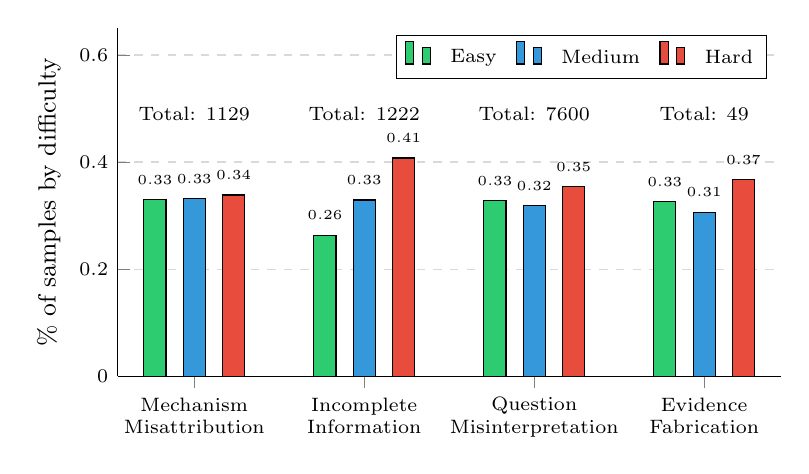
\begin{tikzpicture}[font=\small]
    % Define common colors
    \definecolor{easycolor}{RGB}{46,204,113}
    \definecolor{mediumcolor}{RGB}{52,152,219}
    \definecolor{hardcolor}{RGB}{231,76,60}
    
    \begin{axis}[
        width=10cm,
        height=6cm,
        ybar,
        bar width=8pt,
        ymin=0, ymax=0.65,
        ylabel={\% of samples by difficulty},
        symbolic x coords={MPM, II, MQ, MEF},
        xtick=data,
        xticklabels={
            {Mechanism\\Misattribution},
            {Incomplete\\Information},
            {Question\\Misinterpretation},
            {Evidence\\Fabrication}
        },
        x tick label style={align=center, font=\scriptsize},
        y tick label style={font=\scriptsize},
        legend style={
            at={(0.98,0.98)},
            anchor=north east,
            font=\scriptsize,
            legend columns=-1,
            transpose legend,
            row sep=0pt,
            column sep=5pt
        },
        ymajorgrids=true,
        grid style={dashed, gray!30},
        nodes near coords,
        every node near coord/.append style={
            anchor=south,
            font=\tiny,
            yshift=2pt
        },
        enlarge x limits=0.15,
        axis lines*=left  % This is the key change - only shows left axes
    ]
        \addplot[fill=easycolor, bar shift=-0.5cm] coordinates {
            (MPM, 0.3295) (II, 0.2635) (MQ, 0.3276) (MEF, 0.3265)
        };
        \addplot[fill=mediumcolor, bar shift= 0.00cm] coordinates {
            (MPM, 0.3322) (II, 0.3290) (MQ, 0.3182) (MEF, 0.3061)
        };
        \addplot[fill=hardcolor, bar shift= 0.5cm] coordinates {
            (MPM, 0.3384) (II, 0.4075) (MQ, 0.3542) (MEF, 0.3673)
        };
        \legend{Easy, Medium, Hard}
        
        \node[anchor=south] at (axis cs: MPM, 0.46) {\scriptsize Total: 1129};
        \node[anchor=south] at (axis cs: II, 0.46) {\scriptsize Total: 1222};
        \node[anchor=south] at (axis cs: MQ, 0.46) {\scriptsize Total: 7600};
        \node[anchor=south] at (axis cs: MEF, 0.46) {\scriptsize Total: 49};
        
    \end{axis}
\end{tikzpicture}
\end{document}
    }
    \caption{Statistics of the MedHallu dataset categorized by four categories of hallucinations (see Table \ref{tab:medical_hallucination_types} for detailed definitions) and levels of difficulty (easy, medium, hard).}
    \label{fig:statistics}
\end{figure}
% \textcolor{red}{TL: please show the specific statistics of generated datasets.}
\vspace{-2mm}

\subsection*{Dataset Generation Pipeline}
\vspace{-2mm}
The proposed methodological framework comprises a three-phase pipeline architected for robust hallucinated sample generation (Figure~\ref{fig:pipeline}). 
The pipeline follows a sequential approach: (1) stochastic sampling of potential hallucinated responses based on in-context examples and precise definitions, (2) LLM-based quality filtering mechanisms, (3) correctness checking using bidirectional entailment and LLM prompting. (4) Sequential Improvement via TextGrad. Finally, inspired by~\citep{Hallueval}, we select the most similar sample generated, using semantic similarity in cases where a high-quality sample is not identified. This approach enables comprehensive identification and evaluation of linguistic hallucinations while minimizing false positives through multi-layered verification protocols.

\section{The general case: Proof of \texorpdfstring{\Cref{thm:main-decomp}}{Theorem 1.6}}\label{sec:algo}

First, we show that data structure of \Cref{l:max_min_query} can be used to compute distances witnessed by shortest paths that pass through a constant-size separator.

\begin{lemma}\label{l:single_adhesion}
Fix a constant $k \in \mathbb{N}$. There exists an algorithm which as the input receives an edge-weighted graph $G$ on $n$ vertices and $m$ edges together with a partition of its vertices into three sets $A, B, C$ such that $|B| \leq k$ and there are no edges between $A$ and $C$, and as the output computes $\max_{c \in C} \dist(a, c)$ for every $a \in A$. The running time is $\Oh(m \log n + n \log^{k - 1} n)$.
\end{lemma}

\begin{proof}
Let $B = \{b_1, \ldots, b_k\}$. For any $a \in A, c \in C$, we have $\dist(a, c) = \min_{i \in [k]} \dist(a, b_i) + \dist(c, b_i)$. First, we run Dijkstra's algorithm from every vertex in $B$ to find $\dist(v, b_i)$ for every $v \in V(G)$ and $i \in [k]$. Next, we use \Cref{l:max_min_query} to construct a data structure $\mathbb{D}$ for the point set $\{(\dist(c, b_1), \dots, \dist(c, b_k))\colon c\in C\}\subseteq \mathbb{R}^k$. Now, the value $\max_{c \in C} \dist(a, c)$ for any given $a$ is equal to the answer of $\mathbb{D}$ to the query with argument $(\dist(a, b_1), \dots, \dist(a, b_k))$.
\end{proof}

After computing the distances over a constant-size separator, we will use the following observation to simplify one of the sides of the separation.

\begin{lemma}\label{l:inserting_paths}
Let $G$ be a edge-weighted connected graph and let $A, B, C$ be a partition of its vertices such that there are no edges between $A$ and $C$. For every pair of vertices $u, v \in B$, let $P_{u, v}$ be any shortest path from $u$ to $v$ with all internal vertices in $C$ (assuming such a path exists).

Let $G'$ denote a graph obtained from $G[A \cup B]$ by adding an edge from $u$ to $v$ of weight equal to the length of $P_{u, v}$, for all $u, v \in B$ for which $P_{u, v}$ exists. Then,  $$\dist_G(s, t) = \dist_{G'}(s, t)\qquad\textrm{for all }s,t\in A\cup B.$$
\end{lemma}
\begin{proof}
Let $G''$ be the graph obtained by adding new edges of $G'$ to $G$.
Fix any $s, t \in A \cup B$ and let $P$ denote the shortest path from $s$ to $t$ in $G''$ which minimizes the number of vertices from $C$ visited. Naturally, the weight of $P$ is equal $\dist_G(s, t)$. Assume that such path visits at least one vertex of $C$. Then, the path $P$ is of the form $s \xrightarrow{P_1} x \xrightarrow{P_2} y \xrightarrow{P_3} t$, where $x, y \in B$ and all the internal vertices of $P_2$ are in $C$. By the construction of $G'$, $P_2$ can be replaced with a direct edge from $x$ to $y$ of the same weight. We obtain a same weight path with a smaller number of vertices of $C$ visited, which is a contradiction. Therefore, $P$ is entirely contained in $A \cup B$, hence it exists in $G'$. This shows that $\dist_G(s, t) = \dist_{G'}(s, t)$.
\end{proof}


The next lemma encapsulates the main algorithmic content of the proof of \Cref{thm:main-decomp}. The algorithm will split the tree decomposition provided on input into smaller parts for which the eccentricities are easier to calculate. We use the following lemma to handle a single such part.
\begin{lemma}\label{l:star}
Fix constants $k, g \in \mathbb{N}, 0 < \delta < \frac{1}{54}$. Assume we are given $n \in \mathbb{N}$, an edge-weighted graph $G$ on at most $n$ vertices with a weight function $w \colon E(G) \to \mathbb{N}$, a vertex subset $A$ and a collection of non-empty vertex subsets $V_0, V_1, \dots, V_\ell$ satisfying the following conditions:
\begin{itemize}[nosep]
	\item The sum of weights of all the edges in $G$ is bounded by $\Oh(n)$.
	\item $V(G) \setminus A = V_0 \cup V_1 \cup \dots \cup V_\ell$.
	\item $|A| \leq k$.
	\item For every $i \in [\ell]$, $G[V_i \setminus V_0]$ is connected, $N_G(V_i \setminus V_0) = V_i \cap V_0$, $|V_i| = \Oh(n^\delta)$, and $|V_0 \cap V_i| \leq 4$.
	\item For all $i, j \in [\ell], i \neq j$, $V_i \setminus V_0$ and $V_j \setminus V_0$ are disjoint and non-adjacent in $G$.
	\item Every edge $uv \in E(G)$ with $u, v \not\in A$ is contained in $G[V_i]$ for some $i\in \{0,1,\ldots,\ell\}$.
	\item The graph obtained by taking $G[V_0]$ and adding a clique on $V_0 \cap V_i$ for every $i \in [\ell]$ has Euler genus bounded by $g$.
\end{itemize}
Then, we can compute the eccentricity of every vertex of $G$ in time $\Oh \left( n^{1 + \frac{150 + 54 \delta}{151}} \log^k n \right)$.
\end{lemma}

\begin{proof}
Fix $\delta' = \frac{1 + 97 \delta}{151}$; we have $\delta' - \delta = \frac{1 - 54\delta}{151} > 0$.
Let $E_i$ denote the set of edges with one endpoint in $V_i$ and the other endpoint in $V_i \setminus V_0$. For $i \in [\ell]$, we shall say that $V_i$ is {\em{heavy}} if the sum of weights of $E_i$ is larger than $n^{\delta'}$. Since the sets $E_i$ are pairwise disjoint and the total sum of weights of all the edges is bounded by $\Oh(n)$, the number of heavy subsets is bounded by $\Oh(n^{1 - \delta'})$. Without loss of generality, we may assume that $V_{\ell' + 1}, \dots, V_\ell$ are heavy and $V_1, \dots, V_{\ell'}$ are not, for some $\ell'\in \{0,\ldots,\ell\}$.


For any source vertex $s$, we can calculate distances from $s$ to every vertex of $G$  using breadth first search in time $\Oh(\sum_{e \in E(G)} w(e)) = \Oh(n)$.
In particular, for every $\ell' < i \leq \ell$, we can compute the distances from every vertex of $V_i$ to every vertex of $G$ in total time $\Oh(n^{2 - \delta' + \delta})$, because $$|V_{\ell'+1}\cup \ldots\cup V_{\ell}|\leq n^{1-\delta'}\cdot \Oh(n^\delta)=\Oh(n^{1-\delta'+
\delta}).$$
Additionally, we calculate distances $\dist_G(a, v)$ for every $a \in A, v \in V(G)$ in time $O(n)$.

For every $i \in [\ell]$ and $u,v \in V_0 \cap V_i$, there exists a shortest path $P_{i,u,v}$ from $u$ to $v$ with all internal vertices belonging to $V_i - V_0$ due to the assumption that $G[V_i - V_0]$ is connected and $N_G(V_i - V_0) = V_i \cap V_0$. Therefore, the distance from $u$ to $v$ is bounded by the sum of weights of edges in $E_i$. In particular, for $i \in [\ell']$, $\dist_G(u, v) \leq n^{\delta'}$.

We define $\widetilde{G}$ to be the graph obtained by taking $G[A \cup V_0 \cup \dots \cup V_{\ell'}]$ and applying the following operation for every $i \in \{\ell' + 1, \dots, \ell\}$:
for each pair of vertices $u, v \in A \cup (V_0 \cap V_i)$, add an edge in $\widetilde{G}$ between $u$ and $v$ with weight equal to the total weight of $P_{i,u,v}$. For a fixed $i, u$, we can find $P_{i, u, v}$ for all $v$ using breadth first search in time $\Oh(n)$. Taking a sum over all $i, u$, we get that $\tilde{G}$ can be computed in total time $\Oh(n^{2 - \delta'})$.


\begin{claim}\label{cl:wG}
The sum of the edge weights in $\widetilde{G}$ is $\Oh(n)$. Moreover, for all $u, v \in V(\widetilde{G})$, we have $\dist_{\widetilde{G}}(u, v) = \dist_{G}(u, v)$.
\end{claim}

\begin{proof}
Consider $i \in \{\ell' + 1, \dots, \ell\}$ and any $u, v \in A \cup (V_0 \cap V_i)$ for which we added an edge. Its weight is bounded by the sum of weights of edges in $E_i$. Therefore, the total weight of all edges added is at most
$$
\sum_{i \in \{\ell' + 1, \dots, \ell\}} \left( |A \cup (V_0 \cap V_i)|^2 \sum_{e \in E_i} w(e) \right) \leq (4 + k)^2 \sum_{e \in E(G)} w(e) = \Oh(n).
$$
This proves the first part of the claim.

For the second part of the claim, consider any $i \in \{\ell' + 1, \dots, \ell \}$ and observe that by our assumptions, $A \cup (V_0 \cap V_i)$ separates $(V_0 \cup \dots \cup V_{\ell'} \cup V_{i + 1} \cup \dots \cup V_\ell) \setminus V_i$ from $V_i \setminus V_0$. Hence it suffices to repeatedly apply \Cref{l:inserting_paths}.
\end{proof}

For every $u \in V(\widetilde{G})$, we have $\ecc_G(u) = \max(\ecc_{\widetilde{G}}(v), \max_{v \in V(G) \setminus V(\widetilde{G})} \dist_G(u, v))$. Note, that we already know all the distances $\dist_G(u, v)$ for $v \in V(G) \setminus V(\widetilde{G})$. Similarly, we can already compute $\ecc_G(u)$ for every $u \in V(G) \setminus V(\widetilde{G})$. Therefore, it remains to compute $\ecc_{\widetilde{G}}(v)$ for each $v \in V(\widetilde{G})$. Our goal is to show that this can be done efficiently using \Cref{l:main_ecc}.

Now, let $G'$ be the graph obtained from $\tilde{G}$ by replacing every edge $e$ non-indicent to $A$ with $w(e)\geq 2$ with a path of length $w(e)$ consisting of unit-weight edges. This operation again preserves the distances. Since the sum of edge weights in $\tilde{G}$ is of $\Oh(n)$, the total number of vertices in $G'$ is of $\Oh(n)$. For $0 \leq i \leq \ell'$, we write $V'_i$ to denote the set $V_i$ together with all the vertices added as a part of a path between two endpoints in $V_i$.
As $V_i$ is not heavy for each $i\in [\ell']$, we have
$$
|V'_i \setminus V'_0| \leq |V_i| + \sum_{e \in E_i} w(e) = \Oh(n^{\delta'})\qquad \textrm{for all }i\in [\ell'].
$$

Let $G_0$ denote the graph $G'[V'_0]$ and let $G_0^*$ denote the graph $G'- A$ with $V'_i - V'_0$ contracted to a single vertex $v_i^*$, for each $i \in [\ell']$; note that, all edges of $G_0$ and $G_0^*$ have unit weight.

\begin{claim}
	The graph $G_0^*$ is does not contain $K_{t}$ as a minor, where $t = \Oh(\sqrt{g})$.
\end{claim}

\begin{proof}
Let $\bar{G}_0$ denote the graph obtained by taking $G_0$ and adding a clique on $V_0 \cap V_i$ for every $i \in [\ell']$.
By lemma assumptions and the fact that subdividing edges does not increase the Euler genus, $\bar{G}_0$ has Euler genus at most $g$. In particular, $\bar{G}_0$ is $K_{t'}$-minor-free for some $t' = \Oh(\sqrt{g})$, because the Euler genus of $K_{t'}$ is $\Omega({t'}^2)$.

Similarly, let $\bar{G}_0^*$ be the graph obtained by taking $G_0^*$ and adding a clique on each $V_0 \cap V_i$.
Note, that $\bar{G}_0^* - \{v_1^*, \dots, v_{\ell'}^*\}$ is precisely $\bar{G}_0$. Let $t = \max(t', 6)$.
Recall that a minor model of a clique $K_t$ consists of $t$ pairwise vertex-disjoint connected subgraphs, called
branch sets, such that there is at least one edge between each pair of the branch sets.
Consider a minor model $\varphi$ of $K_{t}$ in $\bar{G}^*_0$.
Note that $\varphi$ cannot contain any singleton branch set of the form $\{v^*_i\}$, for the degree of $v^*_i$ in $\bar{G}^*_0$ is at most $4 < t - 1$. Furthermore, since $N_{\bar{G}^*_0}(v^*_i) = V_0 \cap V_i$, any branch set containing $v^*_i$ and at least one other vertex contains some $u \in V_0 \cap V_i$, and $N_{\bar{G}^*_0}(v^*_i)\subseteq N_{\bar{G}^*_0}(u)$, hence removing $v^*_i$ from this branch set preserves the model. Therefore, we can assume without loss of generality that all branch sets of $\varphi$ are disjoint from $\{v^*_1, \dots, v^*_{\ell'}\}$, hence $\varphi$ is a minor model of $K_{t}$ in $\bar{G}_0$. This is a contradiction, as $t \geq t'$ and $\bar{G}_0$ is $K_{t'}$-minor-free. Therefore, $\bar{G}_0^*$ is $K_t$-minor-free, hence $G_0^*$ also.
\end{proof}

Let $\rho' = \frac{2 - 108 \delta}{151} > 0$. The graph $G^*_0$ is a unit-weight graph and is $K_{t}$-minor-free.
Hence, by applying \Cref{t:r_division} to $G^*_0$ (with $\varepsilon = \rho'/2$)
we obtain an $n^{\rho'}$-division $\mathcal{R}_0$ in time $\Oh(n^{1 + \rho'})$.
We extend it to $G' - A$ by mapping every contracted vertex $v^*_i$ to $N_{G' - A}[V'_i - V'_0] = (V'_i - V'_0) \cup (V_0 \cap V_i)$. Formally, we put $V''_i \coloneqq N_{G' - A}[V'_i - V'_0]$ and 
$$
\mathcal{R} \coloneqq \left\{ (R_0 \cap V'_0) \cup \bigcup_{i \colon v^*_i \in R_0} V''_i \colon R_0 \in \mathcal{R}_0 \right\}.
$$

Now, we argue that $\mathcal{R}$ is a reasonable division of $G' - A$. Clearly, all sets $R \in \mathcal{R}$ are connected in $G' - A$. Pick any $R \in \mathcal{R}$ and let $R_0$ be its corresponding set in $\mathcal{R}_0$.
Every vertex $v^*_i$ is mapped to a set of size $\Oh(n^{\delta'})$, therefore
$$|R| \leq |R_0| \cdot \Oh(n^{\delta'}) = \Oh(n^{\rho' + \delta'}).$$

By our construction, for every $i \in [\ell']$, $R$ is either disjoint from $V'_i - V'_0$ or contains whole $N_{G' - A}[V'_i - V'_0]$. This means that no vertex belonging to any $V'_i - V'_0$ can be in $\partial R$, hence $\partial R \subseteq V'_0$.

Pick any $u \in \partial R \cap R_0$. Assume that $u \not\in \partial R_0$. Then every vertex of $N_{G_0^*}(u)$ must be in $R_0$, hence $N_{G - A'}(u) \subseteq R$, which is a contradiction. This means that $\partial R \cap R_0 \subseteq \partial R_0$.

Pick any $u \in \partial R - R_0$. Then, $u \in V_0 \cap V_i$ for some $i \in [\ell']$ such that $v_i^* \in R_0$. Moreover, $v_i^* \in \partial R_0$ and is adjacent to $u$ in $G_0^*$. The number of such $u$ is bounded by $4 |\partial R_0 \cap \{ v_1^*, \dots, v_{\ell'}^* \}|$.

Putting two cases together, we obtain:
$$
\sum_{R \in \mathcal{R}} |\partial R| = \sum_{R \in \mathcal{R}} \left(|\partial R \cap R_0| + |\partial R - R_0|\right) \leq \sum_{R_0 \in \mathcal{R}_0} \left(|\partial R_0| + 4 |\partial R_0 \cap \{ v_1^*, \dots, v_{\ell'}^* \}|\right) = \Oh(n^{1 - \frac{1}{2}\rho'}).
$$

It remains to show the following claim.

\begin{claim}
Pick any $R \in \mathcal{R}, s_R \in R$. The number of different distance profiles on $R$ relative to $s_R$ in $G' - A$ is of $\Oh(n^{48\rho' + 54\delta'})$.
\end{claim}
\begin{proof}
We look at every vertex $v \in V(G') \setminus A$ and consider three cases: $v \in R$, $v \in V'_0$, and $v \in V'_i \setminus (V'_0 \cup R)$ for some $i \in [\ell']$. By our construction, $R \cap V'_0$ is non-empty, hence w.l.o.g. we can assume that $s_R \in V'_0$ as whether two vertices have the same profile on $R$ is independent of the choice of the pivot vertex.

In the first case, there are at most $|R| = \Oh(n^{\rho' + \delta'})$ such vertices, hence they realise at most that many profiles.

In the second case, we want to observe that profile of any vertex $v \in V'_0$ on $R$ depends only on its profile on $R \cap V'_0$ (relative to $s_R$). Pick any $t \in R - V'_0$. Then $t \in V'_i - V'_0$ for some $i \in [\ell']$, $V_i \cap V_0 \subseteq R \cap V'_0$, and every path from $v$ to $t$ intersects $V_i \cap V_0$. In particular, distances from $v$ to vertices of $V_i \cap V_0$ determine its distance to $t$, which proves the observation.

Let $\tilde{G}_0$ denote the graph obtained by taking $G'[V'_0]$ and for every $i \in [\ell'], u, v \in V_0 \cap V_i$ adding a disjoint path from $u$ to $v$ of length $\dist(u, v)$. Let $P_i$ denote the vertex set of paths added between $V_0 \cap V_i$. For every $t \in V'_0$ we have $\dist_{G' - A}(v, t) = \dist_{\tilde{G}_0}(v, t)$, so it suffices to bound the number of profiles on $R \cap V'_0$ in $\tilde{G}_0$. By our assumptions, $\tilde{G}_0$ has Euler genus bounded by $g$ and all $P_i$ are of size $\Oh(n^{\delta'})$.

Let $R_0$ be the set of $\mathcal{R}_0$ corresponding to $R$. Let $\tilde{R}_0$ denote the set $(R \cap V'_0) \cup \bigcup_{i : v^*_i \in R_0} P_i$. Such set is connected in $\tilde{G}_0$. Moreover, similarly to $R$, its size is $\Oh(n^{\rho' + \delta'})$. Applying \Cref{thm:distprofiles}, we get that the number of distance profiles on $\tilde{R}_0$ in $\tilde{G}_0$ is $\Oh(n^{12(\rho' + \delta')})$, which also bounds the number of profiles on $R$ in $G' - A$ realised by $V'_0$.

For the third case, assume $v \in V'_i \setminus (V'_0 \cup R)$ for some $i\in [\ell']$. Every path from $v$ to any vertex of $R$ in $G' - A$ intersects $V_i \cap V_0$. Let $v_1, \dots v_p$ be the vertices of $V_i \cap V_0$, where $p \leq 4$. The profile of $v$ on $R$ is then determined by the following:
\begin{itemize}[nosep]
 \item[(a)] the profile of each $v_j$ on $R$,
 \item[(b)] $\dist_{G' - A}(v, v_j) - \dist_{G' - A}(v, v_1)$ for each $2 \leq j \leq p$, and
 \item[(c)] $\dist_{G' - A}(s_R, v_j) - \dist_{G' - A}(s_R, v_1)$ for each $2 \leq j \leq p$ where $s_R$ is some pivot vertex of $R$.
\end{itemize}
By the previous case, the number of distance profiles of each $v_j$ is $\Oh(n^{12(\rho' + \delta')})$. The distances between $v$ and $v_j$ are bounded by $|V'_i|$, hence each quantity described in (b) can take $\Oh(n^{\delta'})$ different possible values. Similarly, since $v_1$ and $v_j$ are connected via $V'_i$, $|\dist_{G' - A}(s_R, v_j) - \dist_{G' - A}(s_R, v_1)| \leq \Oh(n^{\delta'})$. The number of different possible profiles of such $v$ is therefore bounded by $\Oh(n^{48(\rho' + \delta') + 6\delta'}) = \Oh(n^{48\rho' + 54\delta'})$. This finishes the proof of the claim.
\end{proof}

Now we can apply \Cref{l:main_ecc} to graph $G'$ with apex set $A$, $X = V(\widetilde{G})$, and the following constants: $$\rho = \rho' + \delta',\qquad \gamma = 1 - \frac{1}{2}\rho',\quad \textrm{and}\quad \alpha = 48\rho' + 54 \delta'.$$ This allows us to calculate all $V(\widetilde{G})$-eccentricities in $G'$ in time
$$
\Oh \left( \left(
	n^{ 2 - \frac{1}{2} \rho' } +
	n^{ 1 + 48\rho' + 54 \delta' }
\right) \log^k n \right) =
\Oh \left( n^{1 + \frac{150 + 54 \delta}{151}} \log^k n \right).
$$
Since for each $v\in V(\widetilde{G})$ we have $\ecc_{\widetilde{G}}(v) = \max_{u \in V(\widetilde{G})} \dist_{\widetilde{G}}(v, u) = \max_{u \in V(\widetilde{G})} \dist_{G'}(v, u)$, this means that we have successfully computed all the eccentricities in $\widetilde{G}$; and as we argued, this is enough to compute all the eccentricities in $G$ as well.

Finally, the total running time of the algorithm is
$$
\Oh \left( n^{1 + \frac{150 + 54 \delta}{151}} \log^k n + n^{2 - \delta' + \delta} \right) =
\Oh \left( n^{1 + \frac{150 + 54 \delta}{151}} \log^k n \right).
$$\qedhere
\end{proof}


\begin{lemma}\label{l:star2}
Fix constants $k, g \in \mathbb{N}, 0 < \delta < \frac{1}{54}$. Assume we are given $n \in \mathbb{N}$, an edge-weighted graph $G$ on at most $n$ vertices with a weight function $w \colon E(G) \to \mathbb{N}$, a vertex subset $A$ and a collection of non-empty vertex subsets $V_0, V_1, \dots, V_\ell$ satisfying the same conditions as in \Cref{l:star} with the following differences:
\begin{itemize}
	\item we don't require $G[V_i - V_0]$ to be connected and $V_i - V_0$ to be adjacent to whole $V_i \cap V_0$;
	\item instead of $|V_0 \cap V_i| \leq 4$, we require $|V_0 \cap V_i| \leq k$.
\end{itemize}
Then, we can compute the eccentricity of every vertex of $G$ in time $\Oh \left( n^{1 + \frac{150 + 54 \delta}{151}} \log^{k + 5g} n \right)$.
\end{lemma}

\begin{proof}
We will reduce our input to one which will satisfy the conditions of \Cref{l:star}. We start by addressing the adhesions $V_0 \cap V_i$ containing too many vertices.

Let $G_0$ denote the graph $G[V_0]$ with cliques placed at $V_0 \cap V_i$ for every $i \in [\ell]$.
For every $i \in [\ell]$ we repeat the following procedure: while $|V_0 \cap V_i| > 4$,
remove arbitrary $5$ vertices from $V_0 \cap V_i$. Since $|V_0 \cap V_i| \leq k$ for each $i\in [\ell]$,
this procedure can be implemented in total time $\Oh(n)$. As a result, at the end we have $|V_0 \cap V_i| \leq 4$ for all $i \in [\ell]$. Let $M$ be the set of all the removed vertices. By our assumptions, $G_0$ has Euler genus bounded by $g$, hence it cannot contain $g + 1$ pairwise disjoint copies of $K_5$
(as the Euler genus of a graph is the sum of the Euler genera of its 2-connected components~\cite{StahlB77} and $K_5$ is not planar). Each removed quintiple of vertices induces a $K_5$ in $G_0$, hence we have $|M| \leq 5g$. We set $A' = A \cup M$ and may thus assume that $V_i$ is disjoint from $A'$ for all $0 \leq i \leq \ell$.

Now, fix $i \in [\ell]$. Let $C^i_1, \dots, C^i_{r_i}$ denote the connected components of $V_i - V_0$ in $G - A'$. We define $W^i_j := N_{G - A'}[C^i_j]$ for every $j \in [r_i]$. Clearly, all $W^i_j$ induce a connected subgraph of $G$ and satisfy $N_{G - A'}(W^i_j - V_0) = W^i_j \cap V_0$. We put $V'_0 := V_0$ and enumerate
$$
\{V'_1, V'_2, \dots V'_{\ell'}\} := \{ W^i_j \colon i \in [\ell], j \in [r_i] \}.
$$
It is easy to verify that the sets $A'$ and $V'_0, V'_1, \dots, V'_{\ell'}$ satisfy the conditions of \Cref{l:star}. We apply said lemma to calculate the eccentricity of every vertex of $G$ in the desired time.
\end{proof}



The next statement is a reformulation of \Cref{thm:main-decomp}.

\begin{theorem}
Fix constants $k, g \in \mathbb{N}$. Assume we are given a graph $G$ on $n$ vertices together with its tree decomposition $(T, \beta)$ and a set of private apices $A_t \subseteq \beta(t)$ for each node $t\in V(T)$ such that the following conditions hold:
\begin{itemize}[nosep]
 \item For every node $t \in V(T)$, we have $|A_t| \leq k$.
 \item For every edge $st \in E(T)$,  we have $|\beta(v) \cap \beta(u)|\leq k$.
 \item For every node $t \in V(T)$, graph obtained by taking $G[\beta(t)] - A_t$ and turning  $(\beta(t) \cap \beta(s))\setminus A_t$ into a clique for every edge $st \in E(T)$ has Euler genus bounded by $g$.
\end{itemize}
Then, we can compute the eccentricity of every vertex of $G$ in time $\Oh \left( n^{1 + \frac{355}{356}} \log^{k + 5g} n \right)$.
\end{theorem}

\begin{proof}
We may assume that $|V(T)|\leq n$, for every tree decomposition with no two bags comparable by inclusion has this property; and adjacent comparable bags can be merged by contracting the edge between them.

For a node $t\in V(T)$, by the {\em{weight}} of $t$ we mean the size of the corresponding bag, that is, $|\beta(t)|$. For any subset of nodes $S \subseteq V(T)$, we define $\beta(S) \coloneqq \bigcup_{t \in S} \beta(t)$ By the {\em{weight}} of $S$, we mean the total weight of the elements of $S$, that is, $\sum_{t\in S} |\beta(t)|$. 

\begin{claim}\label{cl:weight-T}
The weight of $V(T)$ is of $\Oh(n)$.
\end{claim}

\begin{proof}
The sets $\beta'(t) := \beta(t) - \bigcup_{s \in N_T(t)} \beta(s)$ are pairwise disjoint. We have
$$
\sum_{t \in V(T)} |\beta(t)| =
\sum_{t \in V(T)} |\beta'(t)| + 2 \cdot \sum_{st \in E(T)} |\beta(s) \cap \beta(t)| \leq
|V(T)| + 2k|E(T)| = \Oh(n).
$$
\end{proof}

Since every bag induces a graph of bounded Euler genus, the number of edges contained in a bag is linear in its size. In particular, this implies that the total number of edges of $G$ is also bounded by $\Oh(n)$.

We set $$\delta \coloneqq \frac{1}{356}\qquad\textrm{and}\qquad \Delta \coloneqq \frac{355}{356}.$$ Root the tree $T$ in an arbitrarily chosen node; this naturally imposes an ancestor-descendant relation in $T$ (for convenience, every node is considered its own ancestor and descendant).

We start by partitioning $T$ into connected subtrees using the following procedure.
We proceed bottom-up over $T$, processing nodes in any order so that a node is processed after all its strict descendants have been processed. Along the way, we mark some nodes and split the edges of $T$ into heavy and light. Let $t \in V(T)$ be the currently processed non-root node of $T$ and let $e \in E(T)$ be the edge connecting $t$ with its parent. If the total weight of all the unmarked nodes that are descendants of $t$ is at least $n^\delta$ (recall that this includes $t$ itself as well), then we declare $e$ heavy and mark all the descendants of $t$ that were unmarked so far. Otherwise, the edge $e$ is declared light and the procedure proceeds to further nodes of $T$.

Observe that
removing all heavy edges splits $T$ into connected subtrees, say $T'_1, \cdots T'_m$. All of the subtrees, except for possibly the subtree containing the root node, are of weight at least $n^\delta$. In particular, the number of subtrees $m$, and therefore the number of heavy edges, is  bounded by $\Oh(n^{1 - \delta})$. Moreover, in every subtree $T'_i$, removing the node closest to the root splits $T'_i$ into smaller components, each of weight less than $n^\delta$.

Fix a heavy edge $e$ and let $T^e_1$ and $T^e_2$ be the two subtrees into which $T$ splits after removing~$e$. Let $X^e_i = \beta(T^e_i)$ for $i \in \{1, 2\}$. Put $A_e = X^e_1 \setminus X^e_2$, $C_e = X^e_2 \setminus X^e_1$, and $B_e = X^e_1 \cap X^e_2$. By the properties of tree decompositions, such choice of $A_e, B_e, C_e$ satisfies the conditions of \Cref{l:single_adhesion}, hence in time $\Oh(n \log^{k - 1} n)$ we can compute $\max_{v \in X^e_2} \dist_G(u,v)$ for every $u \in X^e_1$, and $\max_{u \in X^e_1} \dist_G(u,v)$ for every $v \in X^e_2$. Computing this for every heavy edge $e$ takes total time $\Oh(n^{2 - \delta} \log^{k - 1} n)$.

Fix any subtree $T'=T'_j$. Let $e_1 = t^{e_1}_1t^{e_1}_2, e_2 = t^{e_2}_1 t^{e_2}_2, \dots, e_\ell = t^{e_\ell}_1 t^{e_\ell}_2$ denote the heavy edges incident to $T'$, where $t^{e_i}_1 \in V(T')$ and $V(T') \subseteq V(T_1^{e_i})$ for every $i \in [\ell]$.
For a vertex $v \in \beta(T')$, let
$$d_0(v) = \max_{u \in \beta(T')} \dist_G(v, u)\qquad\textrm{and}\qquad d_i(v) = \max_{u \in X_2^{e_i}}\dist_G(v,u),\quad\textrm{for } i \in [\ell].$$ We have $\ecc(v) = \max \{ d_i(v)\colon i\in \{0,1,\ldots,\ell\}\}$.The values of $d_i(v)$ are already calculated for all $i\in [\ell]$, hence it remains to compute $d_0(v)$.

For every $i \in [\ell]$ and every pair of vertices $u, v \in \beta(t^{e_i}_1) \cap \beta(t^{e_i}_2)$ we find a shortest path between $u$ and $v$ with all internal vertices inside $X^{e_i}_2$ (or determine that it doesn't exist). For a fixed $u, v$ this can be done in time $\Oh(n)$. Since in total we perform this step at most $2k^2$ times per heavy edge, it takes $\Oh(n^{2 - \delta})$ time in total. Let $P_{i, u, v}$ denote such path, assuming it exists.

Let $G'$ denote the graph obtained from $G[\beta(T')]$ by taking every $i, u, v$ for which $P_{i, u, v}$ exists and adding an edge between $u$ and $v$ of weight equal to the total weight of $P_{i, u, v}$.
The weight of every edge inserted in $\beta(t^{e_i}_1) \cap \beta(t^{e_i}_2)$ is bounded by $|X^{e_i}_2|+1$. The total weight of all edges inserted is therefore at most
$$
\sum_{i \in [\ell]} |\beta(t^{e_i}_1) \cap \beta(t^{e_i}_2)|^2 \cdot (|X^{e_i}_2|+1) \leq
k^2 \sum_{i \in [\ell]} (|X^{e_i}_2|+1) = \Oh(n),
$$
where the last equality follows from the fact that all the trees $T^{e_i}_2$ are pairwise disjoint.
By \Cref{l:inserting_paths}, we have $\dist_{G'}(u, v) = \dist_G(u, v)$ for each $u, v \in \beta(T')$. Hence, computing $d_0(v)$ for every $v \in \beta(T')$ is equivalent to computing the eccentricity of every vertex in $G'$.

If the size of $\beta(T')$ is smaller than $n^\Delta$, we compute the eccentricities naively in time $\Oh(|\beta(T')|^2)$, 
noting that $G'$ has $\Oh(|\beta(T')|)$ edges (thanks to Claim~\ref{cl:weight-T} and bounded genus assumption 
of the last bullet of the theorem statement). Otherwise, we argue that we can use the algorithm in \Cref{l:star} as follows.

Let $t$ be the node of $T'$ closest to the root. Let $s_1, \dots, s_p$ be the children of $t$ in $T$ and let $T''_i$ denote the connected component of $T' - \{t\}$ containing $s_i$. Set $V_0 = \beta(t)$ and $V_i = \beta(T''_i)$ for $i \in [p]$.

It is now easy to verify that $G'$ and sets $A, \{V_i\colon 0\leq i\leq p\}$ selected this way satisfy the assumptions of \Cref{l:star2}. This allows us to use it to compute the eccentricities in $G'$ in time
$$
\Oh \left( n^{1 + \frac{150 + 54\delta}{151}} \log^{k + 5g} n \right) =
\Oh \left( n^{1 + \frac{354}{356}} \log^{k + 5g} n \right).
$$
As we argued, from these eccentricities, we may easily compute all the eccentricities in $G$.

Now, let us analyse the total running time of the whole algorithm. We invoke \Cref{l:star} $\Oh(n^{1 - \Delta})$ times, since we apply it only to subtrees $T'_i$ of size at least $n^\Delta$. The total running time of those applications is hence
$$
\Oh \left( n^{2 + \frac{354}{356} - \Delta} \log^{k + 5g} n \right) =
\Oh \left( n^{1 + \frac{355}{356}} \log^{k + 5g} n \right).
$$
We compute the eccentricities naively for subtrees smaller than $n^\Delta$, hence the total running time of this computation is
$$
\sum_{i \in [m] \colon |\beta(T'_i)| \leq n^\Delta} |\beta(T'_i)|^2 \leq
n^\Delta \cdot \sum_{i \in m} |\beta(T'_i)| = \Oh(n^{1 + \Delta})=\Oh\left(n^{1+\frac{355}{356}}\right).
$$
The rest of computation can be done in $\Oh(n^{2 - \delta} \log^k n)$. Therefore, the whole algorithm runs in time $\Oh \left( n^{1 + \frac{355}{356}} \log^{k + 5g} n \right)$.
\end{proof}


\paragraph{1) Diverse Hallucinated Answer Sampling.} \label{Sampling step}

Using a carefully crafted prompting strategy shown in Figure~\ref{fig:pipeline}, we generate multiple possible hallucinated answers with diverse temperature settings, we describe the prompt in Table~\ref{fig:system_prompt}. Through experiments, we find that allowing the model to choose the category of hallucination to apply to a given medical question performs better than manually forcing a specific hallucination category. For this generation $H_i = LM_i(Q_i,GT_i,C_i)$, we provide the LLM with precise definitions of each category, along with examples, question $Q_i$, and ground truth answers $GT_i$. The LLM is tasked with generating an answer that is semantically similar to ground truth yet incorrect. Additionally, we provide the ground truth context $C_i$, which contains precise knowledge required to answer the question. This includes intricate details necessary for crafting a strong hallucinated answer. 

\paragraph{2) Quality checking - LLM-based Discriminative Filtering.} \label{Quality check}

The second phase of our pipeline implements a comprehensive quality filtering protocol leveraging an ensemble of LLMs to minimize individual model biases. For each generated sample $H_i$, we employ a comparative assessment framework where multiple LLMs independently evaluate two candidate responses: the potentially hallucinated answer and the established ground truth. The quality assessment task is formulated as a binary classification problem, where models are prompted to identify which response appears more factually accurate given the question without access to the ground truth context. To mitigate potential biases from any single model, we implement a majority voting mechanism across different LLM architectures (including Gemma2, GPT-4o-mini, and Qwen2.5). A generated sample $H_i$ is preserved only when at least a majority of models in the ensemble incorrectly identify it as the more accurate response compared to the ground truth.
The difficulty categorization of generated samples is determined by the voting patterns across the LLM ensemble. Specifically, we classify $H_i$ as ``hard'' when all LLMs in the ensemble incorrectly identify it as accurate response, ``medium'' when multiple but not all LLMs are deceived, and ``easy'' when only a single LLM fails to identify the hallucination. This multi-model consensus approach helps ensure that preserved hallucinated samples are sufficiently convincing while reducing the impact of model-specific quirks or biases in the filtering process.
\vspace{-1mm}
\paragraph*{3) Correctness Checking via Entailment.} \label{Correctness check}
We implement a two-stage correctness verification protocol to ensure that the generated hallucinations are semantically distinct from the ground truth while maintaining coherence. First, we employ bidirectional entailment checking using a fine-tuned RoBERTa-large-MNLI model to quantify the semantic divergence between the hallucinated sample $H_i$ and ground truth $GT_i$. The bidirectional entailment score $\mathcal{E}$ is computed as:
$$\mathcal{E}(H_i, GT_i) = \min(\text{NLI}(H_i \rightarrow GT_i), \text{NLI}(GT_i \rightarrow H_i))$$

where $\text{NLI}(x \rightarrow y)$ represents the natural language inference score indicating whether $x$ entails $y$. We establish a stringent threshold $\tau$ and only retain samples that satisfy: $\mathcal{E}(H_i, GT_i) < \tau$. This ensures the hallucinated samples maintain sufficient semantic distance from the ground truth, minimizing false positives while requiring minimal human intervention.


\paragraph*{4) Sequential Improvement via TextGrad.} \label{improvement}
Our framework implements an iterative optimization step to enhance the quality of generated hallucinations that fail initial quality or correctness checks. When a generated sample $H_i$ fails to meet the established quality tests described in Section~\ref{Quality check}, we employ TextGrad optimization to refine subsequent generations through a feedback loop. The optimization process is formalized as: $H_{i+1} = \text{TextGrad}(H_i, F(H_i))$ where $F(H_i)$ represents feedback from the TextGrad optimizer, initialized with GPT-4o-mini. This refinement process (detailed in Section~\ref{Sampling step}) iterates up to five times, terminating either upon reaching a quality-compliant sample or exhausting the iteration limit. For each failed generation, TextGrad analyzes LLM feedback to identify hallucination indicators that make $H_i$ easily detectable. The feedback mechanism specifically focuses on two aspects: (1) linguistic patterns that signal artificial content and (2) structural elements that could be refined to enhance the naturalness. This feedback is then incorporated into subsequent prompt refinement, systematically improving both the content plausibility and stylistic cohesion. If no sample passes the quality filter after maximum iterations, we implement a fallback strategy based on semantic dissimilarity. Specifically, we select the candidate $H_*$ that maximizes the cosine similarity from the ground truth embedding: $H_* = \arg\max_{H_i} (\cos(\text{embed}(H_i), \text{embed}(GT_i)))$. This ensures that even in challenging cases, our pipeline produces outputs with maximum semantic similarity while preserving response coherence.

% \subsection*{Statistics about the MedHallu Dataset}




% \begin{table*}
% \centering
% \small
% \setlength{\tabcolsep}{4pt} % Reduce space between columns
% \begin{tabular}{l|ccccc|ccccc|c}
% \hline
% \textbf{Model} & \multicolumn{5}{c|}{Without Knowledge} & \multicolumn{5}{c|}{With Knowledge} & \textbf{$\Delta$ Know.} \\
% \hline
%               & \shortstack{Overall\\F1} & \shortstack{Overall\\P} & \shortstack{Easy\\F1} & \shortstack{Med\\F1} & \shortstack{Hard\\F1} 
%               & \shortstack{Overall\\F1} & \shortstack{Overall\\P} & \shortstack{Easy\\F1} & \shortstack{Med\\F1} & \shortstack{Hard\\F1} & \\
% \hline
% Qwen2.5-14B-Instruct   & 0.59 & 0.73 & 0.81 & 0.64 & 0.46 & \textbf{0.83} & 0.84 & \textbf{0.93} & 0.89 & 0.74 & +0.24 \\
% Gemma-2-9b-it        & 0.61 & 0.73 & \textbf{0.83} & \textbf{0.73} & 0.44 & 0.81 & 0.78 & 0.88 & 0.85 & \textbf{0.76} & +0.20 \\
% Llama-3.1-8B-Instruct  & 0.44 & \textbf{0.85} & 0.73 & 0.58 & 0.19 & 0.79 & \textbf{0.89} & 0.90 & 0.84 & 0.70 & \textbf{+0.35} \\
% Qwen2.5-7B-Instruct    & 0.51 & 0.73 & 0.78 & 0.58 & 0.31 & 0.81 & 0.85 & 0.92 & 0.83 & 0.74 & +0.30 \\
% Qwen2.5-3B-Instruct    & \textbf{0.62} & 0.47 & 0.66 & 0.67 & \textbf{0.57} & 0.66 & 0.50 & 0.69 & 0.65 & 0.66 & +0.04 \\
% GPT-4o-mini            & 0.55 & 0.78 & 0.81 & 0.65 & 0.35 & \textbf{0.83} & 0.84 & 0.90 & \textbf{0.91} & \textbf{0.76} & +0.28 \\
% DeepSeek-R1-Distill-Llama-8B & 0.51 & 0.61 & 0.64 & 0.62 & 0.40 & 0.77 & 0.83 & 0.87 & 0.80 & 0.69 & +0.26 \\
% \hline
% \textbf{Average (Pre-trained)} & 0.55 & 0.70 & 0.75 & 0.64 & 0.39 & 0.79 & 0.79 & 0.87 & 0.82 & 0.72 & +0.24 \\
% \hline
% \\[-1ex] % extra space before the next header
% \multicolumn{12}{l}{\textbf{Medical Fine-Tuned LLMs}} \\[1ex] % extra space after the header
% \hline
% OpenBioLLM-Llama3-8B & 0.58 & 0.55 & 0.61 & 0.58 & 0.56 & 0.56 & 0.56 & 0.55 & 0.56 & 0.56 & -0.02 \\
% BioMistral-7B       & 0.56 & 0.50 & 0.55 & 0.57 & 0.56 & 0.63 & 0.54 & 0.61 & 0.68 & 0.63 & +0.07 \\
% Llama-3.1-8B-UltraMedical & 0.58 & 0.58 & 0.76 & 0.65 & 0.45 & 0.70 & 0.73 & 0.79 & 0.71 & 0.65 & +0.12 \\
% \hline
% \textbf{Average (Fine-Tuned)} & 0.57 & 0.54 & 0.64 & 0.60 & 0.52 & 0.63 & 0.61 & 0.65 & 0.65 & 0.61 & +0.06 \\
% \hline
% \end{tabular}

% \caption{Performance comparison of different LLMs with and without knowledge. General pre-trained LLMs perform better than Medically fine-tuned LLMs in the task of Medical Hallucination, in terms of almost all metrics. P denotes, Precision. $\Delta$ Know is the performance change in Overall F1 when knowledge is provided to the LLM.}
% \label{tab:llm_performance_merged}
% \end{table*}



\begin{table*}[t]
    \centering
    % Reduce font size globally for this table
    % \scriptsize
    % Adjust row spacing if needed
    \renewcommand{\arraystretch}{1.2}
    % Scale the entire tabular environment to fit within \linewidth
    \begin{adjustbox}{width=1\linewidth, center}
    \begin{tabular}{lccccc|ccccc|c}
    \toprule
    \textbf{Model} & \multicolumn{5}{c|}{\textbf{Without Knowledge}} & \multicolumn{5}{c|}{\textbf{With Knowledge}} & \textbf{$\Delta$ Knowledge} \\
    \cmidrule(lr){1-6} \cmidrule(lr){7-11}
    \textbf{General LLMs} & \textbf{Overall F1} & \textbf{Overall P} & \textbf{Easy F1} & \textbf{Med F1} & \textbf{Hard F1} 
                   & \textbf{Overall F1} & \textbf{Overall P} & \textbf{Easy F1} & \textbf{Med F1} & \textbf{Hard F1} & ($\Delta$ F1)\\
    \cmidrule(lr){2-6} \cmidrule(lr){7-12}
    GPT-4o$^*$                       & \textbf{0.737} & 0.723 & \textbf{0.844} & \textbf{0.758} & \textbf{0.625} & \textbf{0.877} & \textbf{0.882} & \textbf{0.947} & \textbf{0.880} & \textbf{0.811} & 0.140 \\
    GPT-4o mini                  & 0.607 & 0.772 & 0.783 & 0.603 & 0.446 & 0.841 & 0.820 & 0.914 & 0.854 & 0.761 & 0.234 \\
    Qwen2.5-14B-Instruct         & 0.619 & 0.691 & 0.773 & 0.611 & 0.483 & 0.852 & 0.857 & 0.935 & 0.856 & 0.769 & 0.233 \\
    Gemma-2-9b-Instruct          & 0.515 & 0.740 & 0.693 & 0.512 & 0.347 & 0.838 & 0.809 & 0.918 & 0.848 & 0.758 & \textbf{0.323} \\
    Llama-3.1-8B-Instruct        & 0.522 & \textbf{0.791} & 0.679 & 0.515 & 0.372 & 0.797 & 0.775 & 0.880 & 0.796 & 0.722 & 0.275 \\
    DeepSeek-R1-Distill-Llama-8B & 0.514 & 0.570 & 0.589 & 0.515 & 0.444 & 0.812 & 0.864 & 0.895 & 0.794 & 0.751 & 0.298 \\
    Qwen2.5-7B-Instruct          & 0.553 & 0.745 & 0.733 & 0.528 & 0.402 & 0.839 & 0.866 & 0.923 & 0.832 & 0.770 & 0.286 \\
    Qwen2.5-3B-Instruct          & 0.606 & 0.495 & 0.667 & 0.602 & 0.556 &  0.676 & 0.514 & 0.693 & 0.677 & 0.661 & 0.070 \\
    Llama-3.2-3B-Instruct                  & 0.499 & 0.696 & 0.651 & 0.467 & 0.384 & 0.734 & 0.775 & 0.822 & 0.723 & 0.664 & 0.235 \\
    Gemma-2-2b-Instruct                   & 0.553 & 0.620 & 0.680 & 0.524 & 0.457 & 0.715 & 0.786 & 0.812 & 0.705 & 0.631 & 0.162 \\
    
    \midrule
    
    % \multicolumn{12}{l}{\textbf{Medical Fine-Tuned LLMs}} 
    \textbf{Medical Fine-Tuned LLMs} & \textbf{Overall F1} & \textbf{Overall P} & \textbf{Easy F1} & \textbf{Med F1} & \textbf{Hard F1} 
                   & \textbf{Overall F1} & \textbf{Overall P} & \textbf{Easy F1} & \textbf{Med F1} & \textbf{Hard F1} & {($\Delta$ F1)}\\
    \cmidrule(lr){2-6} \cmidrule(lr){7-12}
    OpenBioLLM-Llama3-8B         & 0.484 & 0.490 & 0.494 & 0.474 & 0.483 & 0.424 & 0.567 & 0.438 & 0.412 & 0.423 & -0.060 \\
    BioMistral-7B                & 0.570 & 0.518 & 0.627 & 0.563 & \textbf{0.525} & 0.648 & 0.516 & 0.652 & 0.660 & 0.634 & 0.078 \\
    Llama-3.1-8B-UltraMedical    & \textbf{0.619} & 0.657 & \textbf{0.747} & \textbf{0.596} & 0.524 & 0.773 & 0.679 & 0.832 & 0.777 & \textbf{0.718} & 0.153 \\
    Llama3-Med42-8B & 0.416 & \textbf{0.829} & 0.600 & 0.379 & 0.264 & \textbf{0.797} & \textbf{0.856} & \textbf{0.898} & \textbf{0.794} & 0.707 & \textbf{0.381} \\
    \midrule
    \textbf{Average (General LLMs, w/o GPT-4o)} 
                                 & \textbf{0.533} & \textbf{0.686} & \textbf{0.674} & \textbf{0.517} & 0.412 
                                 & \textbf{0.784} & \textbf{0.789} & \textbf{0.864} & \textbf{0.781} & \textbf{0.716} 
                                 & \textbf{0.251} \\
    \textbf{Average (Medical Fine-Tuned LLMs)} 
                                 & 0.522 & 0.623 & 0.617 & 0.503 & \textbf{0.449} 
                                 & 0.660 & 0.654 & 0.705 & 0.660 & 0.620 
                                 & 0.138 \\
    \bottomrule
    \end{tabular}
    \end{adjustbox}
    \caption{Performance comparison of different LLMs with and without knowledge on MedHallu (10,000 samples). General LLMs perform better than medically fine-tuned LLMs in the task of Medical Hallucination across most metrics. “Overall P” denotes precision, and “\(\Delta\) Knowledge” is the performance change in overall F1 when knowledge is provided. $^*$We exclude GPT-4o while calculating the average to have a fair comparison of model sizes for general vs. fine-tuned LLMs. Additional experimental details can be found in Appendix \ref{Gen_robust_check}.}
    \label{tab:llm_performance_merged}
\end{table*}
\vspace{-2.5mm}
\section{Implementation Details}
\vspace{-2.5mm}
% \paragraph{MedHallu Dataset Generation.} Generating hallucinated responses that preserve semantic alignment with the ground truth while subtly modifying it to outcompete discriminator models is a nuanced challenge.
\paragraph{MedHallu Dataset Generation Settings.} We generate hallucinated responses using \texttt{Qwen2.5B-14B}~\citep{qwen2025qwen25technicalreport}. The ground truth question-answer pairs are sourced from the \texttt{pqa\_labeled} split of PubMedQA~\citep{PubmedQA}, which contains 1,000 expert-annotated samples, supplemented with 9,000 instances randomly selected from the \texttt{pqa\_artificial} split. To achieve high-quality generation with adequate diversity, we utilize regulated sampling settings. The \texttt{temperature} is varied between 0.3 and 0.7, while the \texttt{nucleus sampling threshold (top-p)} is fixed at 0.95. These settings balance cohesion and variability. The maximum response length is capped at 512 tokens to ensure completeness while mitigating computational costs. Each hallucinated answer is limited to within ±10\% of its corresponding ground truth answer's length, ensuring uniform information density.

\noindent $\triangleright$ \textit{Quality \& correctness check.} For quality check, We employ three LLMs: \texttt{GPT-4o mini}~\citep{openai2024gpt4ocard}, \texttt{Gemma2-9B}~\citep{gemmateam2024gemma2improvingopen}, and \texttt{Qwen2.5-7B}~\citep{qwen2025qwen25technicalreport}. A response is retained only if it deceives at least one of these models (see Section~\ref{Quality check}). For \textit{correctness check,} we employ the \texttt{microsoft/deberta-large-mnli} model~\citep{he2021debertadecodingenhancedbertdisentangled},  applying bidirectional entailment with a confidence threshold of 0.75. 

\noindent $\triangleright$ \textit{TextGrad \& Fallback.} We integrate \texttt{TextGrad}~\cite{yuksekgonul2024textgradautomaticdifferentiationtext} with \texttt{GPT-4o mini} as the backend model to generate feedback for samples that fail either the quality or correctness checks. Each sample undergoes a maximum of five generation attempts. If no valid response is produced within these iterations, we adopt a \textbf{fallback strategy}, selecting the most semantically similar generated answer to the ground truth response.

\paragraph{Discriminator Model Settings.} We evaluate a diverse set of model architectures under two distinct settings: (1) \textbf{zero-shot} (without additional knowledge) and (2) \textbf{context-aware} (with ground truth context provision). The detection prompt is described in Figure~\ref{fig:system_prompt_for_detection}. This dual-setting approach allows us to assess both the baseline detection capabilities and the models' ability to leverage contextual information for improved discrimination. We examine both general-purpose and specialized medical models. The \textbf{general models} include \texttt{Gemma-2 (2B, 9B) Instruct}~\citep{gemmateam2024gemma2improvingopen}, \texttt{Llama-3.1 (3B, 8B) Instruct}~\citep{grattafiori2024llama3herdmodels}, \texttt{Qwen-2.5 (3B, 7B, 14B)}~\citep{qwen2025qwen25technicalreport}, \texttt{DeepSeek-R1-Llama 8B}~\citep{deepseekai2025deepseekr1incentivizingreasoningcapability}, \texttt{GPT-4o}, and \texttt{GPT-4o mini}~\citep{openai2024gpt4ocard}. Additionally, we evaluate four \textbf{fine-tuned medical LLMs} such as \texttt{OpenBioLLM-8B}~\citep{OpenBioLLMs}, \texttt{Llama3-Med42-8B}~\citep{christophe2024med42v2suiteclinicalllms}, \texttt{BioMistral-7B}~\citep{labrak2024biomistral}, and \texttt{UltraMedical}~\citep{zhang2024ultramedical} to compare domain-specific adaptations against general-purpose models. In this discriminative task, we maintain a temperature of approximately \texttt{0.2-0.3} for all models. For OpenAI models, we use the official API, while for open-weight models like Llama, Gemma, and Qwen, we utilize the \texttt{Hugging Face Pipeline} to ensure a consistent inference framework across all models.

% \paragraph{Hyperparameter Selection.} \jiawei{I prefer not to have a separate section for hyperparameter selection. We should incorporate it into the two paragraphs above.} To achieve high generation quality with adequate diversity, we utilize regulated sampling settings. The temperature is varied between 0.3 and 0.7, keeping a constant nucleus sampling threshold (top-p) of 0.95. These parameters are empirically optimized to balance between cohesion and variability in responses. For efficiency, the maximum generation length is limited to 512 tokens, ensuring complete responses without undue computational burden. Our experimental design incorporates several model access frameworks for a thorough evaluation. For OpenAI models, we utilize the official API, whereas for open-weight models like Llama, Gemma, and Qwen, we use the Hugging Face Pipeline to maintain uniform inference procedures across all models. To maintain quality control and consistency, we impose certain constraints on generated responses. Each hallucinated answer response must be approximately the same length as its ground truth answer, with a tolerance of ±10\%, to maintain similar information density. Moreover, our generation process is limited to a maximum of 5 attempts per question. If no appropriate response is found within this threshold that passes the quality and correctness check, we switch to our fallback strategy which relies on semantic similarity, as explained in Section~\ref{improvement}.

\section{Results and Analysis} \label{ResultsAnalysis}

% \textcolor{red}{TL: Structurize your results by bullets, and also let the detailed can directly reflect your conclusions.}

% \textcolor{red}{TL: the structure of the experiments part is poor. maybe consider to structure them into all studies related to detection, then generation, then extra research questions.}

% \kaidi{Do we need to compare our results with Med-Halt and/or HaluBench medical part to demonstrate we may have some conflict but reasonable results against theirs? }
\vspace{-2mm}
\subsection{Which language model performs the best at medical hallucination detection task?}

Our experimental results reveal significant variations in hallucination detection performance across model architectures in the zero-shot setting (without relevant knowledge provided). As presented in Table~\ref{tab:llm_performance_merged}, \ding{202}~the size of a model is not necessarily linked to its detection capabilities. For instance, \texttt{Qwen2.5-3B} achieves a high baseline overall F1 score (0.606), outperforming larger models such as \texttt{Gemma-9B} (0.515), \texttt{Llama-3.1-8B-Instruct} (0.522), and even the \texttt{Qwen2.5-7B} model (0.533). \ding{203}~All models exhibit notable performance degradation on ``hard'' samples, with even the best-performing models, such as \texttt{GPT-4o}, showing a significant F1 score drop and achieving only 0.625 in these challenging cases. \ding{204}~An intriguing observation is that, overall, general LLMs outperform medical fine-tuned LLMs in terms of precision and F1 scores in the easy and medium categories when no additional knowledge is provided.

% \section{Ablation Experiments}

% \kaidi{The findings here are more interesting and should be highlighted as xxx-level analysis or other things rather than ablation. We should emphasize only our benchmark can provide such information  }
% We perform an extensive ablation study on the generated samples by measuring performance gains by explicitly providing ground-truth context in the in-context prompt; we note a substantial performance gain in the detection capabilities across LLMs. Yet, the performances of powerful LLMs like Qwen-2.5 14B and Llama-3.1 8B stay in the low 80\%, showing significant scope for performance improvement. We also perform ablation on the generation samples by clustering them. Specifically, we generate 50 possible hallucinated answers for a given question and then cluster them using the bidirectional entailment method proposed in \citep{Farquhar2024DetectingHI_semantic_entropy}. We find that most clusters contain points that either all pass the quality check, leading to high-quality sentences, or all fail the quality check. This highly indicates that these clusters of meaning directly correlate to the quality of the hallucinated sample. Also, across all clusters, we find that the clusters that successfully pass the quality check are closer (measured using Euclidean distance) to the ground truth compared to those with samples that fail the quality check. Similar insights can be derived from other metrics like cosine similarity and rouge score, indicating that cluster meanings and their similarity with ground truth highly affect the quality of hallucination samples generated.
\vspace{-1mm}
\subsection{How does providing knowledge impact detection performance?}
Providing knowledge to the LLMs in this hallucination detection task, yields substantial and consistent improvements in hallucination detection across all evaluated LLM architectures. As shown in Table \ref{tab:llm_performance_merged}, \ding{202} every model benefits from the inclusion of knowledge. In general LLMs, the average overall F1 score increases from 0.533 (without knowledge) to 0.784 (with knowledge), corresponding to a gain of +0.251. In contrast, medically fine-tuned LLMs exhibit a much smaller improvement—from an average overall F1 of 0.522 to 0.660 (+0.138), likely because these models already incorporate specialized domain knowledge during training. Moreover, the scale of the model is pivotal for its performance. \ding{203} Larger structures, such as \texttt{Qwen2.5-14B}, reach an impressive overall F1 score of 0.852 when supplemented with domain knowledge, indicating that their increased capacity supports better text comprehension and integration of knowledge. In contrast, smaller models like \texttt{Qwen2.5-3B} experience just slight enhancement (+0.07 F1, from 0.606 to 0.676), underscoring the variability in how different model sizes effectively use additional information. Remarkably, \texttt{Gemma-2-9B} showed the most significant benefit from knowledge, with its overall F1 score rising from 0.515 to 0.838 (+0.323). Overall, these findings affirm the hypothesis that domain knowledge access improves an LLM's hallucination detection ability, while also emphasizing that both model scale and whether the model has been fine-tuned on medical data are critical to the extent of performance improvements.

% \begin{table}[h]
\footnotesize  % Make the table smaller
\centering
\setlength{\tabcolsep}{4pt}  % Reduce column spacing
\begin{tabular}{l|c|ccc|c}
\hline
\textbf{Model} & \textbf{Overall} & \textbf{Easy} & \textbf{Med} & \textbf{Hard} & $\Delta$ \\
& \textbf{F1} & \textbf{F1} & \textbf{F1} & \textbf{F1} & \textbf{F1} \\
\hline
GPT-4o mini & \textbf{0.83} & 0.94 & 0.85 & 0.76 & +0.26 \\
Qwen2.5-14B & 0.84 & 0.91 & 0.90 & 0.77 & +0.26 \\
Gemma-9B & 0.82 & 0.92 & 0.87 & 0.76 & +0.23 \\
Qwen2.5-7B & 0.81 & 0.89 & 0.85 & 0.74 & +0.29 \\
Gemma-2B & 0.63 & 0.72 & 0.65 & 0.58 & +0.21 \\
Llama-3.1-8B & 0.79 & 0.89 & 0.82 & 0.73 & +0.35 \\
Llama-3.2-3B & 0.64 & 0.72 & 0.71 & 0.56 & +0.28 \\
Qwen2.5-3B & 0.67 & 0.69 & 0.69 & 0.65 & +0.02 \\
\hline
\end{tabular}
\caption{Performance of LLMs with knowledge. $\Delta$ F1 shows the absolute improvement in Overall F1 score compared to no-knowledge setting. Models are sorted by overall F1 score.}
\label{tab:llm_performance_with_2}
\end{table}


\begin{table}
\centering
\small
\begin{tabular}{lccc}
\hline
\textbf{Metric} & \textbf{Mean} & \textbf{Mean} & \textbf{P-value} \\
 & \textbf{(fooled)} & \textbf{(not fooled)} & \\
\hline
Cosine similarity & 0.715 & 0.696 & 0.004 \\
Euclidean distance & 0.714 & 0.750 & 0.002 \\
Rouge1-F1 & 0.358 & 0.319 & 0.002 \\
\hline
\end{tabular}
\caption{The average similarity between the clusters generated in Section \ref{semantic_analysis} and the ground truth samples. Clusters containing samples that fool detection LLMs (i.e., hallucinations that are more challenging to detect) are notably closer to the ground truth.}
\label{tab:metrics_cluster}
\end{table}

\subsection{Semantic analysis of hallucinated and ground truth sentences.} \label{semantic_analysis}
% \jiawei{I feel like this section is different from the previous or later sections. This section is more related to the hallucination generation part. We may need to move this to section 3, as the robust check of our data generation pipeline?}
\vspace{-1mm}
To analyze semantic patterns in hallucinated responses, we conduct a comprehensive clustering analysis on an expanded set of generations. Specifically, we generate 50 candidate hallucinated responses for each question from our sampling phase, as described in Section~\ref{Quality check}. We retain all 50 candidate hallucinated responses, including those that fail the quality or correctness checks, to capture the semantic distribution across both successful and unsuccessful hallucinated answers. Using bidirectional entailment with a threshold of 0.75, we cluster these 50 candidate hallucinated responses along with the ground truth response, forming distinct semantic clusters that represent different conceptual approaches to the same question. This clustering methodology, adapted from~\citep{Farquhar2024DetectingHI_semantic_entropy}, allows us to analyze the semantic structure of hallucinated responses relative to the ground truth, yielding three significant findings:

\paragraph{Cluster-level Detection Patterns.}
Our analysis uncovers a binary discrimination effect within semantic clusters. \ding{202} Specifically, hallucinated responses in the same cluster tend to exhibit near-uniform performance—either consistently passing LLM detection (being favored over the ground truth) or being uniformly flagged as hallucinations. This finding strongly indicates that semantic content, rather than merely surface-level linguistic features, plays a pivotal role in shaping the LLM's discrimination behavior.
\vspace{-1mm}
\paragraph{Cluster Proximity Analysis.}
\ding{203} We find that clusters containing samples that reliably fool detection LLMs (hallucinations that are harder to detect) are notably closer to the ground truth answer in semantic vector space. This closeness is quantified via Euclidean distance, with additional support from cosine similarity and ROUGE scores (Table~\ref{tab:metrics_cluster}). Such proximity suggests that well-crafted hallucinated responses strike a balance, they remain semantically similar enough to the ground truth while incorporating meaningful deviations.

\vspace{-1mm}
\paragraph{Ground Truth Isolation.}
A particularly significant finding is the distinct semantic isolation of ground truth responses from clusters of hallucinated outputs. Empirical evidence demonstrates that ground truth responses rarely, if ever, align within the semantic clusters formed by hallucinations. This clear separation validates the robustness of our generation pipeline, ensuring that hallucinated responses retain semantic distinctness from factual content while upholding contextual relevance.
\begin{table}[h]
\centering
\scriptsize
\begin{tabular}{@{}l c c c c c@{}}
\toprule
\textbf{Model} & \textbf{F1\textsubscript{NS}} & \textbf{P\textsubscript{NS}} & \textbf{F1\textsubscript{R}} & \textbf{P\textsubscript{R}} & \textbf{Response\%} \\ 
\midrule
GPT-4o-mini                     & 66.6  & 66.8 & 60.7 & 77.2 & 98.4   \\
Gemma-2-2b-it                  & 57.1  & 59.9 & 55.3 & 54.1 & 82.7   \\
Llama-3.2-3B-Instruct           & 58.1  & 68.7 & 49.9 & 63.3 & 85.9   \\
Qwen2.5-3B-Instruct             & 65.2  & 67.2 & 60.6 & 50.2 & 65.7   \\
BioMistral-7B                 & 56.5  & 50.5 & 57.0 & 51.3 & 99.2   \\
Qwen2.5-7B-Instruct             & 69.3  & \textbf{94.6} & 55.3 & 73.7 & 47.5   \\
OpenBioLLM-Llama3-8B            & 48.8  & 48.4 & 48.4 & 56.3 & 99.7   \\
Llama-3.1-8B-UltraMedical       & 58.5  & 49.1 & 61.9 & 56.4 & 69.7   \\
DeepSeek-R1-Llama-8B    & 66.0  & 56.9 & 51.4 & 61.7 & 98.1   \\
Llama-3.1-8B-Instruct           & 51.7  & 90.4 & 52.2 & \textbf{86.0} & 98.2   \\
Gemma-2-9b-it                  & 61.4  & 85.5 & 51.5 & 71.5 & 37.6   \\
Qwen2.5-14B-Instruct            & 76.2  & 82.9 & 61.9 & 76.5 & 27.9   \\
GPT-4o                         & \textbf{79.5}  & 79.6 & \textbf{73.7} & 72.4 & 33.9   \\
\bottomrule
\end{tabular}
\caption{F1\textsubscript{NS} and P\textsubscript{NS} (Precision) represent performance with the ``Not Sure'' option, while F1\textsubscript{R} and P\textsubscript{R} (Precision) represent performance when required to answer. Response\% represents the percentage of questions answered with ``Yes'' or ``No'' even when the ``Not Sure'' option is available.}
\label{tab:model-comparison}
\end{table}

\vspace{-5mm}
\subsection{Analysis of models' ability to decline to answer}
% We introduce a ``not sure'' category to the existing ``hallucinated'' and ``not hallucinated'' categories in our detection prompt \jiawei{something like 'Figure S1'} figure \ref{fig:system_prompt_for_detection}. The results (Table \ref{tab:model-comparison}) reveal clear patterns across model sizes and knowledge integration. When models are allowed to express uncertainty, they achieve higher precision but lower recall, effectively maintaining better F1 scores by avoiding low-confidence answers. Different model families show distinct characteristics in handling this trade-off, with Qwen models demonstrating the most consistent performance across both scenarios \jiawei{not true for 'Qwen2.5-14B-Instruct'} , while Llama models show greater variation. Larger models, particularly the 14B and 7B variants, excel in forced-answer scenarios, with Qwen-14B showing remarkable stability. Across both scenarios, knowledge-enabled models consistently outperform their counterparts. Interestingly, 
% \jiawei{What are 'these models?' knowledge-enabled models?} these models appear to use the ``not sure'' option more strategically. The performance gap between knowledge-enabled and knowledge-disabled versions widens when models are required to provide an answer.
% This suggests that enabling the ``not sure'' option benefits applications prioritizing precision, while those requiring higher coverage might benefit from forced answers. 

We introduce a ``not sure'' category alongside the existing ``hallucinated'' and ``not hallucinated'' categories in our detection prompt (Figure \ref{fig:system_prompt_for_detection}), allowing LLMs to decline to answer if they lack full confidence in their responses. Results shown in Table \ref{tab:model-comparison}, reveal that \ding{202} many models demonstrate an improved F1 score and precision when they can opt for ``not sure.'' However, the enhancement varies with model size: smaller models gain a moderate improvement of 3-5\%, whereas larger models see a significant boost of around 10-15\%. General LLMs outperform fine-tuned medical models, with some like GPT-4o achieving up to 79.5\% in performance, and Qwen2.5-14B performing closely at 76.2\%. \ding{203} In terms of the percentage of questions answered with definite ``yes'' or ``no'' (Response Rate), general LLMs respond to fewer questions, with Qwen2.5-14B responding to as little as 27.9\%, reflecting their tendency to skip uncertain questions. Conversely, fine-tuned medical models attempt to answer nearly all questions, rarely selecting the ``Not Sure'' option. This approach sometimes leads to a minor reduction in performance. For instance, UltraMedical's model has the lowest response rate among medical models at 69.7\% , while OpenBioLLM reaches as high as 99.7\%. Finally, \ding{204} when comparing the impact of adding the ``not sure'' choice with knowledge-sharing enhancements, shown in Table \ref{tab:model-comparison-with-knowledge} versus Table \ref{tab:model-comparison}, there is a marked increase in the percentage of questions attempted by General LLMs, suggesting improved confidence in task execution, along with an increase in F1 score and precision.

\begin{figure}
    \centering
    \tiny
    \resizebox{\columnwidth}{!}{
        %Draw graphics
\usepackage{pgfplots}
\usepackage{pgfplotstable}
\pgfplotsset{compat=newest}
\pgfplotscreateplotcyclelist{my chart colors}{%
blue, solid, every mark/.append style={solid, fill=blue}, mark=*\\%
red, solid, every mark/.append style={solid, fill=red}, mark=square*\\%
brown, solid, every mark/.append style={solid, fill=brown}, mark=triangle*\\%
cyan, solid, every mark/.append style={solid, fill=gray}, mark=diamond*\\%
black, dashdotted, every mark/.append style={solid, fill=red}, mark=halfdiamond*\\%
olive, dashdotted, every mark/.append style={solid, fill=green}, mark=halfcircle*\\%
orange, dashdotted, every mark/.append style={solid, fill=gray}, mark=*\\%
purple, dashdotted, every mark/.append style={solid, fill=blue}, mark=halfsquare left*\\%
teal, densely dashed, every mark/.append style={solid, fill=green}, mark=oplus*\\%
violet, densely dashed, every mark/.append style={solid, fill=gray}, mark=diamond*\\%
magenta, densely dashed, every mark/.append style={solid, fill=blue}, mark=triangle*\\%
lime, densely dashed, every mark/.append style={solid, fill=red}, mark=square*\\%
}

\newcommand{\errorband}[5][]{ % x column, y column, error column, optional argument for setting style of the area plot
\pgfplotstableread[col sep=comma, skip first n=2]{#2}\datatable
    % Lower bound (invisible plot)
    \addplot [draw=none, stack plots=y, forget plot] table [
        x={#3},
        y expr=\thisrow{#4}-\thisrow{#5}
    ] {\datatable};

    % Stack twice the error, draw as area plot
    \addplot [draw=none, fill=gray!40, stack plots=y, area legend, #1] table [
        x={#3},
        y expr=2*\thisrow{#5}
    ] {\datatable} \closedcycle;

    % Reset stack using invisible plot
    \addplot [forget plot, stack plots=y,draw=none] table [x={#3}, y expr=-(\thisrow{#4}+\thisrow{#5})] {\datatable};
}
    }
    \caption{Detection accuracy of different hallucination categories on MedHallu, evaluated using \texttt{Qwen2-7B-Instruct} as the discriminator.}
    \label{fig:hallucination_types}
\end{figure}

% \vspace{-9mm}
\subsection{Analysis: Hallucination category and MeSH}

\subsubsection*{Which hallucination category is hardest to detect? }
Our analysis reveals distinct patterns in detection difficulty across hallucination categories, as shown in Figure~\ref{fig:hallucination_types}. \textbf{Incomplete Information (II)} emerges as the most challenging category, with 41\% of total samples being ``hard'' cases (Figure \ref{fig:statistics}) and the lowest detection ratio (54\%), indicating models struggle significantly with validating partial information. \textbf{Mechanism/Pathway Misattribution (MPM)} and \textbf{Question Misinterpretation (MQ)} show notable patterns: MPM has a significant number of hard cases, with a 68\% detection accuracy, while MQ having higher number of hard cases but stronger detection performance (68.8\%). \textbf{Methodological and Evidence Fabrication (MEF)}, despite being the smallest category (37\% are hard), demonstrates the highest detection success rate (76.6\%).

\noindent These findings highlight a crucial insight: subtle manipulation of existing medical information, particularly through incomplete presentation, is harder to detect than outright fabrication. This is evident from II's high difficulty scores compared to MEF's better detection rates. The distribution across difficulty levels (easy, medium, hard) further supports this, with II showing the highest concentration in the ``hard'' category. This suggests that while models excel at identifying completely fabricated information, they struggle with partially accurate yet incomplete medical claims, highlighting critical areas of improvement in hallucination detection systems.

\subsubsection*{Which medical category (MeSH term) hallucination is the hardest to detect?}

\noindent To understand which medical domains are more susceptible to hallucination, we examine the MedHallu dataset with the MeSH categories within the PubMedQA dataset, identifying the top five principal categories shown in Figure~\ref{fig:mesh_categories}. These categories include Diseases (comprising 25.9\% of the samples), Analytical Procedures (20.1\%), Chemical/Drug Queries (15.8\%), Healthcare Management (9.7\%), and Psychiatric Conditions (6.7\%). Detection performance among these categories varies considerably: Disease-related instances exhibit a respectable detection accuracy of 57.1\%, despite the abundance of related medical literature in the corpus. Conversely, Chemical/Drug queries demonstrate the highest detection rate at 67.7\%. In contrast, Psychiatry ranks lowest among the top five categories with a detection rate of just 53.7\%, highlighting the need for further incorporation of this data in the training corpus.

\begin{figure}[t]
    \centering
    \tiny
    \scalebox{0.7}{
        \documentclass{standalone}
\usepackage{tikz}
\usepackage{pgfplots}
\pgfplotsset{compat=1.18}

\begin{document}
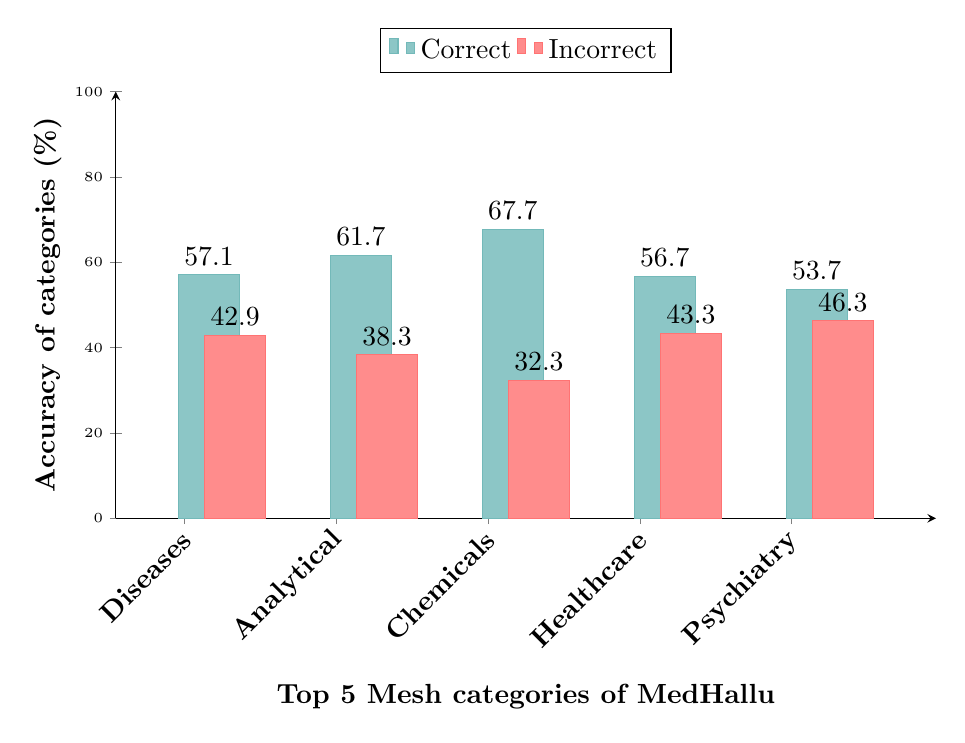
\begin{tikzpicture}
\tiny
\begin{axis}[
    width=12cm,
    height=7cm,
    ybar=-40pt,    % Reduced from 8pt to bring bars closer
    bar width=22pt,
    ylabel={\normalsize\textbf{Accuracy of categories (\%)}},
    xlabel={\normalsize\textbf{Top 5 Mesh categories of MedHallu}},
    xlabel style={yshift=-1em}, 
    symbolic x coords={D1,D2,A1,A2,C1,C2,H1,H2,P1,P2},
    xtick={D1,A1,C1,H1,P1},
    xticklabels={\normalsize\textbf{Diseases}, \normalsize\textbf{Analytical}, \normalsize\textbf{Chemicals}, \normalsize\textbf{Healthcare}, \normalsize\textbf{Psychiatry}},
    xticklabel style={
        rotate=45,           % Rotates labels 45 degrees
        anchor=east,         % Aligns the labels properly
        yshift=-0.5em        % Adjusts vertical position
    },
    legend style={
        at={(0.5,1.15)},
        anchor=north,
        legend columns=2,
        font=\normalsize
    },
    ymin=0,
    ymax=100,   % Changed to a percentage scale
    axis lines=left,
    clip=false,
    enlarge x limits=0.1,  % Reduced side margins
    nodes near coords,
    nodes near coords style={font=\normalsize},
    every node near coord/.append style={yshift=1pt}
]

% Calculated percentages (rounded to one decimal place):
% Diseases: Correct: 148/259*100 ≈ 57.1, Incorrect: 111/259*100 ≈ 42.9
% Analytical: Correct: 124/201*100 ≈ 61.7, Incorrect: 77/201*100 ≈ 38.3
% Chemicals: Correct: 107/158*100 ≈ 67.7, Incorrect: 51/158*100 ≈ 32.3
% Healthcare: Correct: 55/97*100 ≈ 56.7, Incorrect: 42/97*100 ≈ 43.3
% Psychiatry: Correct: 36/67*100 ≈ 53.7, Incorrect: 31/67*100 ≈ 46.3

\addplot[fill=teal!45!white, draw=teal!55!white] coordinates {
    (D1,57.1) (A1,61.7) (C1,67.7) (H1,56.7) (P1,53.7)
}; \addlegendentry{Correct}

\addplot[fill=red!45!white, draw=red!55!white] coordinates {
    (D2,42.9) (A2,38.3) (C2,32.3) (H2,43.3) (P2,46.3)
}; \addlegendentry{Incorrect}

\label{Mesh_class_plot}
\end{axis}
\end{tikzpicture}
\end{document}
    }
    \caption{Detection accuracy across Mesh categories proposed in PubMedQA. We use \texttt{Qwen2.5-7B-Instruct} as a discriminator for the 1k samples of MedHallu generated on pqa\_labeled split.}
    \label{fig:mesh_categories}
\end{figure}

\vspace{-2mm}
\section{Conclusion}
\vspace{-2mm}
We introduce MedHallu, a comprehensive benchmark comprising 10,000 rigorously curated medical question-answer pairs with hallucinated answers. MedHallu integrates fine-grained categorization of medical hallucination types, a hallucination generation framework that balances difficulty levels while mitigating single-LLM bias through multi-model majority voting, and systematically evaluates diverse LLM configurations' hallucination detection capabilities. Our evaluation reveals that existing LLMs exhibit significant limitations in detecting medical hallucinations, particularly struggling with "hard" hallucination answers, which are closer in distance to the ground truth. We also provide insights into enhancing LLMs' hallucination detection: when knowledge is provided, general-purpose LLMs can outperform medical fine-tuned models, and allowing models to decline to answer by providing a "not sure" option improves precision in critical applications. As the largest open medical hallucination benchmark to date, MedHallu serves as a valuable resource for evaluating LLMs' medical hallucination detection abilities and offers insights into the cautious use of LLMs in high-stakes medical domains.


\section{Limitations}
Our study faces three primary constraints. First, due to resource constraints, we could not employ the most advanced reasoning models (e.g., OpenAI o1, Gemini 2.0, DeepSeek-R1) for benchmark generation. While our pipeline incorporates multi-stage LLM quality checks and regeneration steps, using state-of-the-art models would incur prohibitive computational costs. Second, our evaluation of LLMs was restricted to input-output prompting (zero-shot, with/without knowledge provision); resource limitations precluded exploration of advanced techniques like chain-of-thought or self-consistency, which might better elicit model capabilities. Third, our hallucination generation pipeline relied on the PubMedQA corpus to ensure contextual fidelity. While this ensures biomedical relevance, future work should incorporate diverse high-quality corpora to improve scalability and domain coverage.

\section{Ethics Statement}
This research adheres to rigorous ethical standards in dataset creation and evaluation. The MedHallu benchmark utilizes publicly available PubMedQA data under MIT licenses, ensuring proper attribution and compliance with source terms of use. Patient privacy is preserved through the exclusive use of de-identified biomedical literature. While our work aims to improve AI safety in healthcare, we acknowledge potential dual-use risks and advocate for responsible deployment of medical LLMs with human oversight. The benchmark's stratification enables targeted mitigation of dangerous ``hard'' hallucinations that most closely resemble factual content. All artifacts will be released with detailed documentation to promote transparency and reproducibility in medical AI safety research.


% This work introduces MedHallu, a comprehensive benchmark for evaluating medical hallucination detection capabilities in large language models. Through our systematic evaluation of 50,000 question-answer pairs across various medical domains, we have uncovered several critical insights about the current state and limitations of hallucination detection in medical AI systems.
% Our findings demonstrate that even state-of-the-art language models struggle with medical hallucination detection, achieving only moderate performance in zero-shot settings (F1 scores of 0.65 or lower). The provision of ground truth context significantly improves detection capabilities across all models, with some achieving F1 scores up to 0.84, highlighting the crucial role of knowledge grounding in enhancing model reliability. However, the persistent challenges in detecting ``hard'' cases, particularly those involving incomplete information, underscore the complexity of this task and the need for continued advancement in model architectures and training approaches.

% The semantic clustering analysis revealed that hallucination detection is primarily influenced by semantic content rather than surface-level features, with clear patterns emerging in how models evaluate responses within similar semantic clusters. This finding suggests that future improvements in hallucination detection should focus on enhancing models' semantic understanding capabilities rather than purely syntactic features.

% These findings have significant implications for deploying AI systems in healthcare settings. The substantial improvement in detection performance, when models are provided with ground truth context (+35\% F1 score in some cases), suggests that future medical AI systems should be designed with robust knowledge integration capabilities. Additionally, the benefits of allowing models to express uncertainty (``not sure'' option) in improving precision highlights the importance of implementing appropriate confidence thresholds in clinical applications.

% As AI systems become increasingly integrated into healthcare decision-making processes, the ability to reliably detect and filter out hallucinated information becomes crucial. The MedHallu benchmark provides a foundation for evaluating and improving these capabilities, contributing to developing more reliable and trustworthy medical AI systems.

% \bibliographystyle{acl_natbib}
\bibliography{bib} 

\clearpage

\appendix
% ----------------------------------------------
\newpage
\section*{supplementary material}
In this supplementary material, we will provide a theoretical analysis to the proposed memory efficient Transformer adapter (META) in Section~\ref{secS1}, provide a detailed description of the experimental datasets in Section~\ref{secS2}, provide a detailed description of the experimental settings in Section~\ref{secS3},
provide more result comparisons under different pre-trained weights in Section~\ref{secS4},
provide more ablation study results in Section~\ref{secS5}, show class activation map comparisons of instance segmentation before and after adding the Conv branch in Section~\ref{secS6},qualitative visualizations of instance segmentation and semantic segmentation results in Section~\ref{secS7},  as well as the pseudo-code for when the stripe size is set to $2$ in Section~\ref{secS8}. 
% -------------------------------------------
\section{Theoretical Analysis of META}
\label{secS1}
% -------------------------------------------
{\color{red}{\emph{This supplementary is for Section~3 of the main paper.}}} In this section, we will prove that META exhibits superior generalization capability and stronger adaptability compared to existing ViT adapters. 
%
To achieve this goal, we will prove that the proposed memory efficient adapter (MEA) block possesses larger information entropy (IE) than the existing attention-based ViT adapters~\citep{hu2022lora,jie2023fact,chen2022vision,ma2024segment,luo2023forgery,shao2023deepfake}, which provides evidence that the MEA block has more comprehensive feature representations. Then, based on the maximum mean discrepancy (MMD) theory~\citep{cheng2021neural,arbel2019maximum,wang2021rethinking}, larger IE in the ViT adapter framework leads to superior generalization capability and stronger adaptability. The detailed theoretical analysis process is as follows:

\begin{lemma}
% ---------------------------------
In any case of mutual information, the MEA block will gain larger information entropy after fusing $\textbf{X}_{vit}$ and $\textbf{X}_{con}$.
% ---------------------------------
\end{lemma}
% ---------------------------------
\begin{proof}
As introduced in Section~3.2 of the main paper, the proposed MEA block can be viewed as an operation that integrates the ViT features (\ie, the Attn branch and the FFN branch) and the convolution features (\ie, the Conv branch). Therefore, we begin by formalizing the obtained features into the following two basic elements: the ViT features and the convolution features. To formalize the learning setting, we express the ViT features as $\textbf{X}_{vit}$ and the convolution features as $\textbf{X}_{con}$. It is evident that if $\textbf{X}_{vit}$ and $\textbf{X}_{con}$ are extracted from the same image, then $\textbf{X}_{vit}$ and $\textbf{X}_{con}$ are not independently distributed, and there exists some mutual information between them~\citep{zhang2022graph,wu2021cvt,zhang2023cae,peng2021conformer}. Therefore, the IE of the fused feature of $\textbf{X}_{vit}$ and $\textbf{X}_{con}$ within the MEA block can be expressed as:
% ---------------------------------------------------
\begin{equation}
\begin{split}
\label{eqs:1}
\textrm{H}(\textbf{X}_{vit}, \textbf{X}_{con}) = \textrm{H}(\textbf{X}_{vit}) + \textrm{H}(\textbf{X}_{con}) - \textrm{I}(\textbf{X}_{vit}; \textbf{X}_{con}),
\end{split}
\end{equation}
% ---------------------------------------------------
where $\textrm{H}(\cdot)$ is utilized to calculate the IE of the given variate, which can be formulated as:
% ---------------------------------------------------
\begin{equation}
\begin{split}
\label{eqs:2}
\textrm{H}(\textbf{X}_{vit}) = -\sum P(\textbf{x}_{vit}) log(P(\textbf{x}_{vit})),\\
\textrm{H}(\textbf{X}_{con}) = -\sum P(\textbf{x}_{con}) log(P(\textbf{x}_{con})),
\end{split}
\end{equation}
% ---------------------------------------------------
where $P(\textbf{x}_{vit})$ represents the probability of $\textbf{X}_{vit}$ taking on the value of $\textbf{x}_{vit}$. The similar definition of $P(\textbf{x}_{con})$. $\textrm{I}(\cdot;\cdot)$ in Eq.~\eqref{eqs:1} is used to compute the mutual information between $\textbf{X}_{vit}$ and $\textbf{X}_{con}$, which can be expressed as:
% ---------------------------------------------------
\begin{equation}
\begin{split}
\label{eqs:3}
\textrm{I}(\textbf{X}_{vit}; \textbf{X}_{con}) = \sum\sum \textrm{P}(\textbf{X}_{vit}, \textbf{X}_{con}) \textrm{log}(\textrm{P}(\textbf{X}_{vit}, \textbf{X}_{con}) (\textrm{P}(\textbf{X}_{vit}), \textrm{P}(\textbf{X}_{con}))),
\end{split}
\end{equation}
% ---------------------------------------------------
where $\textrm{P}(\textbf{X}_{vit}, \textbf{X}_{con})$ is their joint probability distribution. 
%\textrm{P}(\textbf{X}_{vit})$ and $\textrm{P}(\textbf{X}_{con})$ are the marginal probability distributions of $\textbf{X}_{vit}$ and $\textbf{X}_{con}$, respectively. 
Since $\textrm{I}(\textbf{X}_{vit}; \textbf{X}_{con})$ is always non-negative, $\textrm{H}(\textbf{X}_{vit}, \textbf{X}_{con})$ may still be greater than $\textrm{H}(\textbf{X}_{vit})$ or $\textrm{H}(\textbf{X}_{con})$~\citep{paninski2003estimation,gabrie2018entropy}. This suggests that the IE of the features extracted by MEA is always greater than the feature representation extracted by either of them separately.

Specifically, if $\textrm{I}(\textbf{X}_{vit}; \textbf{X}_{con})$ is small, the IE gain after fusion may still be significant, which is beneficial for improving the generalization capability and adaptability of the block. However, when $\textrm{I}(\textbf{X}_{vit}; \textbf{X}_{con})$ is large, the IE gain after fusion may be reduced. This means that $\textrm{I}(\textbf{X}_{vit}; \textbf{X}_{con})$ may affect the IE improvement of the fused model. Next, we will discuss the impact of $\textbf{X}_{vit}$ and $\textbf{X}_{con}$ on improving the IE of the adapter based on the size of $\textrm{I}(\textbf{X}_{vit}; \textbf{X}_{con})$, which can be divided into the following three cases:

\begin{itemize}
% --------------------------
\item {{Small} $\textrm{I}(\textbf{X}_{vit}; \textbf{X}_{con})$.} This is an ideal state. When the dependency between $\textbf{X}_{vit}$ and $\textbf{X}_{con}$ is small, it indicates that $\textrm{I}(\textbf{X}_{vit}; \textbf{X}_{con})$ is small, that is, $\textbf{X}_{vit}$ and $\textbf{X}_{con}$ respectively represent different information of the image. In this case, fusing $\textbf{X}_{vit}$ and $\textbf{X}_{con}$ can bring a significant increase in IE, which is beneficial to improving the adapter's generalization capability and adaptability.
% --------------------------
\item {{Medium} $\textrm{I}(\textbf{X}_{vit}; \textbf{X}_{con})$.} When $\textrm{I}(\textbf{X}_{vit}; \textbf{X}_{con})$ is between small and large, it indicates that there is a certain degree of correlation between them. In this case, fusing $\textbf{X}_{vit}$ and $\textbf{X}_{con}$ may still bring some IE gain. The specific improvement effect depends on the degree of correlation between $\textbf{X}_{vit}$ and $\textbf{X}_{con}$ and their complementarity in image representations. Fortunately~\citep{zhang2022graph,zhang2023cae,marouf2024mini,liu2023efficientvit}, a large amount of work has validated that ViT and convolutional layers can extract distinctive information from images. Therefore, in this case, fusing $\textbf{X}_{vit}$ and $\textbf{X}_{con}$ can still bring IE gains.
\item {{Large} \myparagraph{$\textrm{I}(\textbf{X}_{vit}; \textbf{X}_{con})$}.} When $\textrm{I}(\textbf{X}_{vit}; \textbf{X}_{con})$ between $\textbf{X}_{vit}$ and $\textbf{X}_{con}$ is large, it indicates that there is a high correlation between them, \ie, global ViT and local convolution features may represent similar or overlapping information of the image. In this case, the IE gain brought by fusing $\textbf{X}_{vit}$ and $\textbf{X}_{con}$ may decrease because there is a lot of information overlap between them. However, in our case, the probability of such a scenario occurring is almost non-existent, fusing $\textbf{X}_{vit}$ and $\textbf{X}_{con}$ may still improve the performance of the model to some extent, because they may capture the detailed information of the image to varying degrees.
% --------------------------
\end{itemize}
% --------------------------

Based on the aforementioned theoretical analysis, we can conclude that the proposed MEA block has a larger IE than existing ViT adapters (which are primarily based on the attention mechanism) under any scenario. This provides evidence that the MEA block has more comprehensive feature representations. 
% ---------------------------------
\end{proof}
% ---------------------------------
As the MEA block includes a parallel convolutional branch, it can better capture local inductive biases compared to the traditional ViT adapter, which mainly uses self-attention~\citep{hu2022lora,jie2023fact,chen2022vision,ma2024segment,luo2023forgery,shao2023deepfake,mercea2024time}. 
%
Therefore, the MEA block's feature space should be more capable of distinguishing different samples, resulting in a larger MMD value. 
%
Our MEA block's feature space is obtained by combining the attention branch, the feed-forward network branch, and the local convolutional branch, enabling it to capture both local and global inductive biases of the given image. 
%
In contrast, the traditional ViT adapter's feature space is mainly obtained through self-attention and may not be able to capture local features well. Therefore, according to the MMD theory~\citep{cheng2021neural,arbel2019maximum,wang2021rethinking}, we can conclude that if the MEA block's feature space is more discriminative than the traditional ViT adapter's feature space, then the MEA block's feature space is more suitable for adapter feature space and can better improve the model's generalization capability and adaptability.

% -------------------------------------------
\section{Introduction of the Experimental Datasets}
\label{secS2}
% -------------------------------------------
{\color{red}{\emph{This supplementary is for Section~4.1 of the main paper.}}}
In our paper, two representative datasets are used to evaluate the effectiveness and efficiency of our method, including MS-COCO~\citep{caesar2018coco} for ODet and ISeg, and ADE20K~\citep{zhou2017scene} for SSeg. Below are the details of the used datasets:

% -------------------------------
\begin{itemize}
% -------------------------------
\item MS-COCO~\citep{caesar2018coco} is a representative yet challenging dataset for common scene IS and object detection, which consists of $118$k, $5$k and $20$k images for the \emph{training} set, the \emph{val} set and the \emph{test} set, respectively. In our experiments, the model is trained on the \emph{training} set and evaluated on the \emph{val} set.
% -------------------------------
\item ADE20K~\citep{zhou2017scene} is a scene parsing dataset with $20$k images and $150$ object categories. Each image has pixel-level annotations for SS of objects and regions within the scene. The dataset is divided into $20$k, $2$k, and $3$k images for \emph{training}, \emph{val} and \emph{test}, respectively. Our model is trained on the \emph{training} set and evaluated on the \emph{val} set.
% -------------------------------
\end{itemize}
% -------------------------------
For data augmentation, random horizontal flip, brightness jittering and random scaling within the range of $[0.5, 2]$ are used in training as in~\citep{chen2022vision,luo2023forgery,zhang2023cae,mercea2024time}. By default, the inference results are obtained at a single scale, unless explicitly specified otherwise.    


% -------------------------------------------
\section{Introduction of the Experimental Settings}
\label{secS3}
% -------------------------------------------
{\color{red}{\emph{This supplementary is for Section~4.2 of the main paper.}}} Experiments on object detection and instance segmentation are conducted using the open-source MMDetection framework~\citep{chen2019mmdetection}. The training batch size is set to $16$, and AdamW~\citep{loshchilov2017decoupled} is used as the optimizer with the initial learning rate of $1 \times 10^{-4}$ and the weight decay of $0.05$. The layer-wise learning rate decay is used and set to $0.9$, and the drop path rate is set to $0.4$. Following~\citep{xiong2024efficient,wang2021pyramid,chen2022vision,liu2022convnet}, to ensure a fair result comparison, we choose two training schedules, 1$\times$ (\ie, $12$ training epochs) and 3$\times$ (\ie, $36$ training epochs). For the 1$\times$ training schedule, images are resized to the shorter side of 800 pixels, with the longer side not exceeding $1,333$ pixels. In inference, the shorter side of images is consistently set to 800 pixels by default. For the 3$\times$ training schedule, the multi-scale training strategy is also used as in~\citep{chen2022vision}, and the shorter side is resized to $480$ to $800$ pixels, while the longer side remains capped at $1,333$ pixels.

{\color{red}{\emph{This supplementary is for Section~4.3 of the main paper.}}} Experiments on semantic segmentation are conducted using the MMSegmentation framework~\citep{mmseg2020}. The input images are cropped to a fix size of 512 $\times$ 512 pixels as in~\citep{xiong2024efficient,chen2022vision}. The training batch size is set to $16$, and AdamW~\citep{loshchilov2017decoupled} is used as the optimizer with the initial learning rate of $1 \times 10^{-5}$ and the weight decay of $0.05$. Following~\citep{li2022exploring,liu2021swin}, the layer-wise learning rate decay is set to $0.9$ and the drop path rate is set to $0.4$. We report the experimental results on both single scale training and multi-scale training strategies. 
% -------------------------------
\begin{table}[t]
\centering
\small
\renewcommand\arraystretch{1.2}
\setlength{\tabcolsep}{6pt}{
\begin{tabular}{r|r|ccl}
\hline \hline 
Methods & Pre-Trained & Params.$\downarrow$ & AP$^\textrm{m}$ $\uparrow$ \\
\hline 
Swin-B~\citep{liu2021swin} & ImageNet-1k~\citep{deng2009imagenet} & 107.1 &  43.3 \\
ViT-Adapter-B~\citep{chen2022vision} & ImageNet-1k~\citep{deng2009imagenet} & 120.2 & 43.6 \\
\cellcolor[gray]{.95}\textbf{META-B$_{{\textrm{(Ours)}}}$} & \cellcolor[gray]{.95}ImageNet-1k~\citep{deng2009imagenet} & \cellcolor[gray]{.95}115.3 & \cellcolor[gray]{.95}44.3$_{\color{red}{+0.7}}$ \\
\cdashline{1-4}[0.8pt/2pt]
Swin-B~\citep{liu2021swin} & ImageNet-22k~\citep{steiner2021train} & 107.1 & 44.3\\
ViT-Adapter-B~\citep{chen2022vision} & ImageNet-22k~\citep{steiner2021train} & 120.2 & 44.6 \\
\cellcolor[gray]{.95}\textbf{META-B$_{{\textrm{(Ours)}}}$} & \cellcolor[gray]{.95}ImageNet-22k~\citep{steiner2021train} & \cellcolor[gray]{.95}115.3  & \cellcolor[gray]{.95}45.2$_{\color{red}{+0.6}}$ \\
\cdashline{1-4}[0.8pt/2pt]
Swin-B~\citep{liu2021swin} & Multi-Modal~\citep{zhu2022uni} & 107.1 &   -- \\
ViT-Adapter-B~\citep{chen2022vision} & Multi-Modal~\citep{zhu2022uni} & 120.2  & 45.3 \\
\cellcolor[gray]{.95}\textbf{META-B$_{{\textrm{(Ours)}}}$} & \cellcolor[gray]{.95}Multi-Modal~\citep{zhu2022uni} & \cellcolor[gray]{.95}115.3  & \cellcolor[gray]{.95}45.9$_{\color{red}{+0.6}}$ \\
\hline \hline 
\end{tabular}
\caption{Result comparisons on Params. (\textbf{M}) and AP (\%) under different pre-trained weights with Mask R-CNN ($3 \times$ +MS schedule)~\citep{he2017mask} as the baseline model on the \emph{val} set of MS-COCO~\citep{caesar2018coco}. ``--'' denotes there is no such a result in its paper.}
\label{tab3}}
\end{table}
% -------------------------------

% -------------------------------------------
\section{Result Comparisons under Different Weights}
\label{secS4}
% -------------------------------------------
{\color{red}{\emph{This supplementary is for Section~4.2 of the main paper.}}} In this section, we present the experimental results of META on object detection and instance segmentation with different pre-trained weights and compare them with other state-of-the-art methods including SwinViT~\citep{liu2021swin} and ViT-Adapter~\citep{chen2022vision} as in~\citep{chen2022vision}. 
Mask R-CNN~\citep{he2017mask} is used as the baseline, and ViT-B~\citep{li2022exploring} is used as the backbone. The 3$\times$ training schedule with MS training strategy is used. The obtained experimental results are given in Table~\ref{tab3}.
%
From this table, we can observe that our method is applicable to different pre-trained weights (\ie, ImageNet-1k~\citep{deng2009imagenet}, ImageNet-22k~\citep{steiner2021train}, and Multi-Modal~\citep{zhu2022uni}), and achieves more accurate AP with fewer model parameters compared to ViT-Adapter~\citep{chen2022vision}, across different pre-trained weights.  

% -------------------------------------------
\section{More Ablation Study Results}
\label{secS5}
% -------------------------------------------
{\color{red}{\emph{This supplementary is for Section~4.4 of the main paper.}}} In our main paper, we present the experimental results of deploying adapters with Attn branch and FFN branch as components on ViT-B~\citep{li2022exploring}. It is noteworthy that the layer normalization operation has been shared between the Attn branch and the FFN branch to reduce the memory access costs associated with the normalization operations. In this section, we demonstrate a result comparison between the experimental results of using shared layer normalization operation and those of not using it in the traditional setting (\ie, the non-shared normalization). The obtained experimental results are shown in Table~\ref{tab:s1}. It can be observed that sharing layer normalization does not significantly improve the performance in terms of AP. However, compared to FPS, FLOPs, MC, our approach can achieve satisfactory performance gains.
% --------------------------
\begin{table*}[t]
\centering
\renewcommand\arraystretch{1.2}
\setlength{\tabcolsep}{1pt}{
\begin{tabular}{r|ccccc|ccccc}
\hline \hline 
Settings & ViT-B & Attn & FFN & Conv & Cascade & AP$^\textrm{m}$ $\uparrow$ & FPS$\uparrow$ & Params.$\downarrow$ & FLOPs$\downarrow$ & MC$\downarrow$ \\
\hline 
Baseline model & \cmark & \xmark & \xmark & \xmark & \xmark & 41.3 & 11.5 & 113.6\textbf{M} & 719\textbf{G} & NA\\
\cdashline{1-11}[0.8pt/2pt]
\cellcolor[gray]{.95}Shared normalization & \cmark & \cmark & \cmark & \xmark & \xmark & \cellcolor[gray]{.95}43.4 & \cellcolor[gray]{.95}11.3 & \cellcolor[gray]{.95}114.4\textbf{M} & \cellcolor[gray]{.95}719\textbf{G} & \cellcolor[gray]{.95}7.5\textbf{GB}\\
Non-shared normalization & \cmark & \cmark & \cmark & \xmark & \xmark & 43.2 & 10.5 & 114.4\textbf{M} & 737\textbf{G} & 8.8\textbf{GB}\\
\hline \hline 
\end{tabular}
\caption{Ablation study results on shared layer normalization.}
\label{tab:s1}}
\end{table*}
% --------------------------

% -------------------------------
{\color{red}{\emph{This supplementary is for Section~4.4 of the main paper.}}} META is proposed as a simple and fast ViT adapter by minimizing inefficient memory access operations. In this section, we compare META with other efficient attention methods and advanced adapter methods~\citep{marouf2024mini,xia2022vision,sung2022vl}. All methods are used with their default settings and the same settings as the injector and extractor in ViT-adapter~\citep{chen2022vision}. Following the same setup as in~\citep{chen2022vision}, the attention mechanism is utilized as the ViT-adapter layer. Therefore, during the experimental comparisons, we replace the attention mechanism in the ViT-adapter with alternative attention mechanisms to ensure a fair comparison. 
The obtained experimental results are given in Table~\ref{tab6}. We can observe that compared to these methods, META achieves new state-of-the-art performance in both accuracy and efficiency. We ultimately achieve an AP of $44.3\%$ with $115.3$\textbf{M} parameters, $720$\textbf{G} FLOPs, $17.4$ FPS, and 8.1 \textbf{GB} MC. 
% -------------------------------
\begin{table}[t]
\centering
\footnotesize
\renewcommand\arraystretch{1.2}
\setlength{\tabcolsep}{5pt}{
\begin{tabular}{r|ccccc}
\hline \hline 
Methods & AP$\uparrow$ & FPS$\uparrow$ & Params. (\textbf{M})$\downarrow$ & FLOPs (\textbf{G})$\downarrow$  & Momory (\textbf{GB})$\downarrow$ \\
\hline 
WindowAtt~\citep{liu2021swin} & 41.2 & 11.6 & 145.0 & 982 & 18.5 \\
PaleAttention~\citep{wu2022pale} & 42.8 & 14.4 & 155.2 & 1,029 & 16.7\\
Attention~\citep{vaswani2017attention} & 43.1 & 5.2 & 188.4 & 1,250 & 18.3 \\
CSWindow~\citep{dong2022cswin}& 43.1 & 13.7 & 144.6 & 990 & 12.9\\
SimplingAtte~\citep{he2023simplifying} & 43.3 & 12.2 & 126.3 & 994 & 17.1\\
DeformableAtt~\citep{xia2022vision} & 43.7 & 13.5 & 166.0 & 988 & 15.2 \\
\cdashline{1-6}[0.8pt/2pt]
MiniAdapters~\citep{marouf2024mini} & 41.9 & 15.0 & 131.8 & 995 & 12.2 \\
VL-Adapter~\citep{sung2022vl} & 42.7 & 14.5 & 167.2 & 993  & 14.0\\
\cellcolor[gray]{.95}\textbf{META-B$_{{\textrm{(Ours)}}}$} & \cellcolor[gray]{.95}44.3 & \cellcolor[gray]{.95}17.4 & \cellcolor[gray]{.95}115.3 & \cellcolor[gray]{.95}720 & \cellcolor[gray]{.95}8.1\\
\hline \hline 
\end{tabular}
\caption{Result comparisons with different adapters.}
\label{tab6}}
\end{table}
% -------------------------------

% -------------------------------------------
\section{Visualizations under the Conv branch}
\label{secS6}
% -------------------------------------------
{\color{red}{\emph{This supplementary is for Section~3.2 of the main paper.}}} In this section, to observe if the adapter has learned local inductive biases through the Conv branch, we visualize the model's class activation maps. The obtained visualizations are given in Figure~\ref{figs1}. From this figure, it can be observed that after adding the Conv branch, the model focuses more on the specific object area (\eg,`` the dog'' and ``the person'') rather than the surrounding area that may extend beyond the object itself, as was the case before adding the Conv branch. This indicates that our method effectively learns local inductive biases after incorporating the Conv branch.
% -------------------------------------------
% This file was created by matlab2tikz.
%
%The latest updates can be retrieved from
%  http://www.mathworks.com/matlabcentral/fileexchange/22022-matlab2tikz-matlab2tikz
%where you can also make suggestions and rate matlab2tikz.
%
\definecolor{mycolor1}{rgb}{0.21569,0.54902,0.72157}%
\definecolor{mycolor2}{rgb}{0.80784,0.16863,0.12157}%
%
\begin{tikzpicture}

\begin{axis}[%
width=0.898in,
height=1.5in,%3.603in,
at={(0.766in,0.486in)},
scale only axis,
xmin=0,
xmax=10,
ymin=0,
ymax=0.8,
xlabel= \phantom{$z$},
ylabel=$p(g_{z^*}|Y)$,
ylabel near ticks,
title={Linearization-based\\ approach},
title style={align=left}, 
axis background/.style={fill=white},
axis x line*=bottom,
axis y line*=left,
legend style={legend cell align=left, align=left, draw=white!15!black}
]
\addplot[ybar interval, fill=mycolor1, fill opacity=0.4, draw=mycolor1, area legend] table[row sep=crcr] {%
x	y\\
3.36	0.0144927536231884\\
3.429	0.0289855072463768\\
3.498	0.0869565217391305\\
3.567	0.217391304347825\\
3.636	0.391304347826087\\
3.705	0.565217391304348\\
3.774	0.449275362318841\\
3.843	0.405797101449276\\
3.912	0.666666666666667\\
3.981	0.420289855072464\\
4.05	0.478260869565218\\
4.119	0.289855072463768\\
4.188	0.289855072463768\\
4.257	0.347826086956522\\
4.326	0.246376811594203\\
4.395	0.304347826086953\\
4.464	0.20289855072464\\
4.533	0.217391304347823\\
4.602	0.246376811594203\\
4.671	0.289855072463768\\
4.74	0.246376811594203\\
4.809	0.188405797101449\\
4.878	0.231884057971015\\
4.947	0.27536231884058\\
5.016	0.391304347826087\\
5.085	0.246376811594203\\
5.154	0.27536231884058\\
5.223	0.217391304347826\\
5.292	0.347826086956518\\
5.361	0.231884057971018\\
5.43	0.2463768115942\\
5.499	0.260869565217395\\
5.568	0.275362318840576\\
5.637	0.289855072463772\\
5.706	0.304347826086953\\
5.775	0.289855072463772\\
5.844	0.362318840579706\\
5.913	0.289855072463768\\
5.982	0.463768115942029\\
6.051	0.420289855072464\\
6.12	0.492753623188406\\
6.189	0.463768115942029\\
6.258	0.463768115942029\\
6.327	0.420289855072459\\
6.396	0.246376811594206\\
6.465	0.202898550724635\\
6.534	0.0869565217391316\\
6.603	0.0579710144927529\\
6.672	0.0289855072463772\\
6.741	0.0144927536231882\\
6.81	0.0144927536231882\\
};
%\addlegendentry{ground truth}

\addplot [color=mycolor2, line width=2.0pt]
  table[row sep=crcr]{%
0	0.00495647934021539\\
0.01	0.00503120737369003\\
0.02	0.00510691052511148\\
0.03	0.00518359894024572\\
0.04	0.00526128282899922\\
0.05	0.00533997246516116\\
0.06	0.00541967818613227\\
0.07	0.00550041039264009\\
0.08	0.00558217954844049\\
0.09	0.00566499618000535\\
0.1	0.00574887087619621\\
0.11	0.00583381428792371\\
0.12	0.00591983712779276\\
0.13	0.00600695016973323\\
0.14	0.006095164248616\\
0.15	0.00618449025985429\\
0.16	0.00627493915898998\\
0.17	0.00636652196126503\\
0.18	0.0064592497411776\\
0.19	0.0065531336320228\\
0.2	0.00664818482541805\\
0.21	0.0067444145708128\\
0.22	0.0068418341749824\\
0.23	0.00694045500150619\\
0.24	0.00704028847022945\\
0.25	0.00714134605670927\\
0.26	0.00724363929164408\\
0.27	0.00734717976028668\\
0.28	0.00745197910184082\\
0.29	0.00755804900884096\\
0.3	0.00766540122651533\\
0.31	0.00777404755213196\\
0.32	0.00788399983432761\\
0.33	0.00799526997241961\\
0.34	0.00810786991570027\\
0.35	0.00822181166271396\\
0.36	0.00833710726051655\\
0.37	0.00845376880391716\\
0.38	0.00857180843470236\\
0.39	0.00869123834084212\\
0.4	0.00881207075567811\\
0.41	0.00893431795709363\\
0.42	0.00905799226666551\\
0.43	0.00918310604879767\\
0.44	0.00930967170983618\\
0.45	0.00943770169716588\\
0.46	0.00956720849828854\\
0.47	0.00969820463988202\\
0.48	0.00983070268684103\\
0.49	0.00996471524129867\\
0.5	0.0101002549416293\\
0.51	0.0102373344614323\\
0.52	0.0103759665084967\\
0.53	0.0105161638237465\\
0.54	0.0106579391801673\\
0.55	0.0108013053817126\\
0.56	0.010946275262192\\
0.57	0.0110928616841387\\
0.58	0.0112410775376588\\
0.59	0.0113909357392594\\
0.6	0.0115424492306589\\
0.61	0.0116956309775763\\
0.62	0.0118504939685016\\
0.63	0.0120070512134457\\
0.64	0.0121653157426715\\
0.65	0.012325300605404\\
0.66	0.012487018868522\\
0.67	0.0126504836152284\\
0.68	0.0128157079437017\\
0.69	0.0129827049657272\\
0.7	0.0131514878053083\\
0.71	0.0133220695972577\\
0.72	0.0134944634857689\\
0.73	0.0136686826229678\\
0.74	0.0138447401674437\\
0.75	0.0140226492827617\\
0.76	0.0142024231359536\\
0.77	0.0143840748959895\\
0.78	0.0145676177322305\\
0.79	0.0147530648128596\\
0.8	0.0149404293032943\\
0.81	0.0151297243645786\\
0.82	0.0153209631517556\\
0.83	0.0155141588122201\\
0.84	0.0157093244840515\\
0.85	0.0159064732943274\\
0.86	0.0161056183574168\\
0.87	0.016306772773255\\
0.88	0.0165099496255975\\
0.89	0.0167151619802561\\
0.9	0.0169224228833143\\
0.91	0.017131745359324\\
0.92	0.0173431424094836\\
0.93	0.0175566270097958\\
0.94	0.0177722121092072\\
0.95	0.0179899106277294\\
0.96	0.0182097354545399\\
0.97	0.018431699446066\\
0.98	0.0186558154240489\\
0.99	0.0188820961735898\\
1	0.0191105544411779\\
1.01	0.0193412029326999\\
1.02	0.0195740543114314\\
1.03	0.0198091211960107\\
1.04	0.0200464161583947\\
1.05	0.0202859517217969\\
1.06	0.0205277403586084\\
1.07	0.0207717944883015\\
1.08	0.0210181264753159\\
1.09	0.0212667486269282\\
1.1	0.0215176731911045\\
1.11	0.0217709123543368\\
1.12	0.0220264782394623\\
1.13	0.0222843829034672\\
1.14	0.0225446383352741\\
1.15	0.0228072564535138\\
1.16	0.0230722491042814\\
1.17	0.0233396280588773\\
1.18	0.0236094050115328\\
1.19	0.0238815915771207\\
1.2	0.0241561992888519\\
1.21	0.0244332395959568\\
1.22	0.0247127238613533\\
1.23	0.0249946633592999\\
1.24	0.0252790692730363\\
1.25	0.0255659526924097\\
1.26	0.0258553246114888\\
1.27	0.026147195926164\\
1.28	0.0264415774317359\\
1.29	0.0267384798204914\\
1.3	0.0270379136792673\\
1.31	0.0273398894870028\\
1.32	0.0276444176122807\\
1.33	0.0279515083108568\\
1.34	0.0282611717231799\\
1.35	0.0285734178718998\\
1.36	0.0288882566593667\\
1.37	0.0292056978651199\\
1.38	0.0295257511433677\\
1.39	0.0298484260204579\\
1.4	0.0301737318923396\\
1.41	0.0305016780220172\\
1.42	0.0308322735369956\\
1.43	0.0311655274267189\\
1.44	0.0315014485400004\\
1.45	0.0318400455824475\\
1.46	0.0321813271138789\\
1.47	0.032525301545736\\
1.48	0.0328719771384891\\
1.49	0.0332213619990379\\
1.5	0.0335734640781073\\
1.51	0.0339282911676388\\
1.52	0.034285850898178\\
1.53	0.0346461507362581\\
1.54	0.0350091979817809\\
1.55	0.0353749997653947\\
1.56	0.0357435630458696\\
1.57	0.0361148946074719\\
1.58	0.0364890010573359\\
1.59	0.0368658888228363\\
1.6	0.0372455641489584\\
1.61	0.0376280330956701\\
1.62	0.0380133015352924\\
1.63	0.0384013751498731\\
1.64	0.0387922594285599\\
1.65	0.0391859596649766\\
1.66	0.0395824809546015\\
1.67	0.0399818281921483\\
1.68	0.040384006068951\\
1.69	0.0407890190703521\\
1.7	0.0411968714730958\\
1.71	0.0416075673427256\\
1.72	0.0420211105309874\\
1.73	0.0424375046732393\\
1.74	0.0428567531858665\\
1.75	0.0432788592637046\\
1.76	0.0437038258774694\\
1.77	0.0441316557711956\\
1.78	0.0445623514596833\\
1.79	0.0449959152259539\\
1.8	0.0454323491187165\\
1.81	0.0458716549498434\\
1.82	0.0463138342918566\\
1.83	0.0467588884754263\\
1.84	0.047206818586881\\
1.85	0.0476576254657295\\
1.86	0.0481113097021966\\
1.87	0.0485678716347722\\
1.88	0.0490273113477746\\
1.89	0.0494896286689283\\
1.9	0.0499548231669573\\
1.91	0.0504228941491942\\
1.92	0.0508938406592059\\
1.93	0.0513676614744362\\
1.94	0.0518443551038658\\
1.95	0.0523239197856913\\
1.96	0.0528063534850216\\
1.97	0.0532916538915952\\
1.98	0.0537798184175165\\
1.99	0.0542708441950129\\
2	0.0547647280742127\\
2.01	0.0552614666209458\\
2.02	0.0557610561145651\\
2.03	0.0562634925457924\\
2.04	0.0567687716145866\\
2.05	0.0572768887280368\\
2.06	0.0577878389982796\\
2.07	0.0583016172404419\\
2.08	0.0588182179706094\\
2.09	0.0593376354038221\\
2.1	0.0598598634520962\\
2.11	0.0603848957224738\\
2.12	0.0609127255151013\\
2.13	0.0614433458213363\\
2.14	0.0619767493218837\\
2.15	0.0625129283849627\\
2.16	0.063051875064503\\
2.17	0.0635935810983738\\
2.18	0.0641380379066434\\
2.19	0.0646852365898719\\
2.2	0.0652351679274361\\
2.21	0.0657878223758891\\
2.22	0.0663431900673527\\
2.23	0.0669012608079454\\
2.24	0.0674620240762456\\
2.25	0.0680254690217902\\
2.26	0.06859158446361\\
2.27	0.0691603588888017\\
2.28	0.0697317804511384\\
2.29	0.0703058369697168\\
2.3	0.070882515927644\\
2.31	0.0714618044707637\\
2.32	0.0720436894064212\\
2.33	0.0726281572022699\\
2.34	0.0732151939851174\\
2.35	0.0738047855398146\\
2.36	0.0743969173081847\\
2.37	0.0749915743879969\\
2.38	0.0755887415319811\\
2.39	0.0761884031468874\\
2.4	0.0767905432925892\\
2.41	0.0773951456812309\\
2.42	0.0780021936764202\\
2.43	0.0786116702924671\\
2.44	0.0792235581936674\\
2.45	0.079837839693634\\
2.46	0.0804544967546748\\
2.47	0.0810735109872175\\
2.48	0.0816948636492834\\
2.49	0.0823185356460092\\
2.5	0.0829445075292169\\
2.51	0.0835727594970344\\
2.52	0.084203271393565\\
2.53	0.0848360227086074\\
2.54	0.0854709925774259\\
2.55	0.0861081597805728\\
2.56	0.0867475027437606\\
2.57	0.0873889995377879\\
2.58	0.0880326278785163\\
2.59	0.0886783651269002\\
2.6	0.0893261882890704\\
2.61	0.0899760740164704\\
2.62	0.0906279986060465\\
2.63	0.0912819380004926\\
2.64	0.0919378677885496\\
2.65	0.0925957632053583\\
2.66	0.0932555991328697\\
2.67	0.0939173501003085\\
2.68	0.0945809902846947\\
2.69	0.0952464935114191\\
2.7	0.0959138332548775\\
2.71	0.0965829826391593\\
2.72	0.0972539144387952\\
2.73	0.0979266010795609\\
2.74	0.0986010146393384\\
2.75	0.0992771268490357\\
2.76	0.0999549090935642\\
2.77	0.100634332412874\\
2.78	0.101315367503047\\
2.79	0.101997984717452\\
2.8	0.102682154067954\\
2.81	0.103367845226185\\
2.82	0.104055027524874\\
2.83	0.104743669959238\\
2.84	0.105433741188425\\
2.85	0.106125209537028\\
2.86	0.106818042996652\\
2.87	0.107512209227537\\
2.88	0.108207675560252\\
2.89	0.108904408997439\\
2.9	0.109602376215622\\
2.91	0.110301543567076\\
2.92	0.111001877081754\\
2.93	0.111703342469276\\
2.94	0.112405905120979\\
2.95	0.113109530112027\\
2.96	0.113814182203577\\
2.97	0.114519825845015\\
2.98	0.115226425176241\\
2.99	0.115933944030024\\
3	0.116642345934409\\
3.01	0.117351594115192\\
3.02	0.118061651498449\\
3.03	0.118772480713129\\
3.04	0.119484044093701\\
3.05	0.120196303682873\\
3.06	0.120909221234355\\
3.07	0.121622758215693\\
3.08	0.122336875811159\\
3.09	0.123051534924699\\
3.1	0.123766696182943\\
3.11	0.124482319938267\\
3.12	0.125198366271925\\
3.13	0.12591479499723\\
3.14	0.126631565662796\\
3.15	0.127348637555838\\
3.16	0.128065969705534\\
3.17	0.128783520886434\\
3.18	0.129501249621939\\
3.19	0.130219114187826\\
3.2	0.130937072615837\\
3.21	0.131655082697321\\
3.22	0.132373101986931\\
3.23	0.133091087806378\\
3.24	0.133808997248241\\
3.25	0.13452678717983\\
3.26	0.135244414247106\\
3.27	0.135961834878651\\
3.28	0.136679005289694\\
3.29	0.137395881486191\\
3.3	0.138112419268956\\
3.31	0.138828574237848\\
3.32	0.139544301796001\\
3.33	0.140259557154114\\
3.34	0.14097429533479\\
3.35	0.141688471176923\\
3.36	0.142402039340136\\
3.37	0.143114954309265\\
3.38	0.143827170398901\\
3.39	0.144538641757969\\
3.4	0.145249322374359\\
3.41	0.145959166079606\\
3.42	0.146668126553618\\
3.43	0.147376157329438\\
3.44	0.148083211798065\\
3.45	0.148789243213316\\
3.46	0.149494204696722\\
3.47	0.150198049242482\\
3.48	0.150900729722448\\
3.49	0.151602198891158\\
3.5	0.152302409390905\\
3.51	0.153001313756856\\
3.52	0.153698864422194\\
3.53	0.154395013723319\\
3.54	0.155089713905069\\
3.55	0.155782917125992\\
3.56	0.156474575463644\\
3.57	0.157164640919932\\
3.58	0.157853065426486\\
3.59	0.158539800850068\\
3.6	0.15922479899801\\
3.61	0.159908011623694\\
3.62	0.160589390432051\\
3.63	0.161268887085104\\
3.64	0.16194645320753\\
3.65	0.16262204039226\\
3.66	0.163295600206099\\
3.67	0.163967084195381\\
3.68	0.164636443891645\\
3.69	0.165303630817341\\
3.7	0.165968596491557\\
3.71	0.166631292435772\\
3.72	0.167291670179631\\
3.73	0.167949681266742\\
3.74	0.168605277260496\\
3.75	0.169258409749901\\
3.76	0.169909030355445\\
3.77	0.170557090734967\\
3.78	0.171202542589549\\
3.79	0.171845337669428\\
3.8	0.17248542777992\\
3.81	0.173122764787353\\
3.82	0.173757300625023\\
3.83	0.174388987299154\\
3.84	0.175017776894874\\
3.85	0.1756436215822\\
3.86	0.176266473622029\\
3.87	0.176886285372142\\
3.88	0.177503009293208\\
3.89	0.178116597954805\\
3.9	0.178727004041434\\
3.91	0.179334180358544\\
3.92	0.179938079838555\\
3.93	0.180538655546892\\
3.94	0.181135860688006\\
3.95	0.181729648611403\\
3.96	0.182319972817676\\
3.97	0.182906786964519\\
3.98	0.183490044872755\\
3.99	0.184069700532347\\
4	0.184645708108407\\
4.01	0.185218021947199\\
4.02	0.185786596582135\\
4.03	0.186351386739756\\
4.04	0.186912347345709\\
4.05	0.187469433530713\\
4.06	0.188022600636505\\
4.07	0.188571804221778\\
4.08	0.189117000068111\\
4.09	0.189658144185865\\
4.1	0.190195192820082\\
4.11	0.190728102456354\\
4.12	0.191256829826677\\
4.13	0.191781331915283\\
4.14	0.192301565964453\\
4.15	0.192817489480306\\
4.16	0.193329060238567\\
4.17	0.193836236290307\\
4.18	0.194338975967659\\
4.19	0.19483723788951\\
4.2	0.195330980967159\\
4.21	0.195820164409952\\
4.22	0.196304747730887\\
4.23	0.196784690752181\\
4.24	0.197259953610816\\
4.25	0.197730496764038\\
4.26	0.198196280994839\\
4.27	0.198657267417387\\
4.28	0.19911341748243\\
4.29	0.199564692982658\\
4.3	0.200011056058033\\
4.31	0.200452469201067\\
4.32	0.200888895262076\\
4.33	0.201320297454377\\
4.34	0.201746639359454\\
4.35	0.202167884932071\\
4.36	0.202583998505353\\
4.37	0.202994944795806\\
4.38	0.203400688908302\\
4.39	0.203801196341013\\
4.4	0.204196432990295\\
4.41	0.204586365155525\\
4.42	0.204970959543887\\
4.43	0.205350183275104\\
4.44	0.205724003886121\\
4.45	0.206092389335735\\
4.46	0.206455308009166\\
4.47	0.206812728722581\\
4.48	0.207164620727553\\
4.49	0.207510953715471\\
4.5	0.207851697821886\\
4.51	0.208186823630804\\
4.52	0.208516302178914\\
4.53	0.208840104959761\\
4.54	0.209158203927852\\
4.55	0.209470571502708\\
4.56	0.209777180572843\\
4.57	0.210078004499687\\
4.58	0.210373017121445\\
4.59	0.210662192756884\\
4.6	0.21094550620906\\
4.61	0.211222932768978\\
4.62	0.211494448219179\\
4.63	0.211760028837266\\
4.64	0.212019651399358\\
4.65	0.212273293183472\\
4.66	0.212520931972839\\
4.67	0.212762546059146\\
4.68	0.212998114245707\\
4.69	0.213227615850562\\
4.7	0.213451030709505\\
4.71	0.213668339179034\\
4.72	0.21387952213923\\
4.73	0.214084560996561\\
4.74	0.214283437686611\\
4.75	0.214476134676732\\
4.76	0.214662634968617\\
4.77	0.214842922100803\\
4.78	0.215016980151093\\
4.79	0.215184793738895\\
4.8	0.21534634802749\\
4.81	0.21550162872622\\
4.82	0.215650622092589\\
4.83	0.215793314934298\\
4.84	0.215929694611184\\
4.85	0.216059749037091\\
4.86	0.216183466681654\\
4.87	0.216300836572001\\
4.88	0.21641184829438\\
4.89	0.21651649199569\\
4.9	0.216614758384949\\
4.91	0.21670663873466\\
4.92	0.216792124882109\\
4.93	0.21687120923057\\
4.94	0.216943884750432\\
4.95	0.21701014498024\\
4.96	0.217069984027651\\
4.97	0.21712339657031\\
4.98	0.217170377856636\\
4.99	0.217210923706529\\
5	0.21724503051199\\
5.01	0.217272695237652\\
5.02	0.217293915421236\\
5.03	0.217308689173911\\
5.04	0.217317015180578\\
5.05	0.217318892700066\\
5.06	0.217314321565234\\
5.07	0.217303302183007\\
5.08	0.217285835534308\\
5.09	0.217261923173913\\
5.1	0.217231567230225\\
5.11	0.217194770404953\\
5.12	0.217151535972715\\
5.13	0.217101867780549\\
5.14	0.217045770247346\\
5.15	0.216983248363191\\
5.16	0.216914307688628\\
5.17	0.21683895435383\\
5.18	0.216757195057696\\
5.19	0.216669037066854\\
5.2	0.216574488214588\\
5.21	0.216473556899676\\
5.22	0.216366252085147\\
5.23	0.216252583296955\\
5.24	0.216132560622568\\
5.25	0.216006194709479\\
5.26	0.215873496763628\\
5.27	0.215734478547749\\
5.28	0.21558915237963\\
5.29	0.215437531130296\\
5.3	0.215279628222107\\
5.31	0.215115457626779\\
5.32	0.214945033863324\\
5.33	0.21476837199591\\
5.34	0.214585487631638\\
5.35	0.21439639691825\\
5.36	0.21420111654175\\
5.37	0.213999663723949\\
5.38	0.213792056219935\\
5.39	0.213578312315465\\
5.4	0.213358450824282\\
5.41	0.213132491085352\\
5.42	0.212900452960033\\
5.43	0.212662356829162\\
5.44	0.212418223590075\\
5.45	0.212168074653546\\
5.46	0.211911931940665\\
5.47	0.211649817879627\\
5.48	0.211381755402469\\
5.49	0.21110776794172\\
5.5	0.210827879426989\\
5.51	0.210542114281486\\
5.52	0.210250497418463\\
5.53	0.209953054237604\\
5.54	0.209649810621332\\
5.55	0.209340792931057\\
5.56	0.209026028003361\\
5.57	0.208705543146111\\
5.58	0.208379366134512\\
5.59	0.2080475252071\\
5.6	0.207710049061664\\
5.61	0.207366966851112\\
5.62	0.207018308179279\\
5.63	0.206664103096667\\
5.64	0.206304382096132\\
5.65	0.205939176108512\\
5.66	0.205568516498194\\
5.67	0.20519243505863\\
5.68	0.204810964007791\\
5.69	0.204424135983574\\
5.7	0.204031984039149\\
5.71	0.203634541638252\\
5.72	0.203231842650435\\
5.73	0.202823921346256\\
5.74	0.202410812392424\\
5.75	0.201992550846891\\
5.76	0.201569172153899\\
5.77	0.201140712138983\\
5.78	0.200707207003916\\
5.79	0.200268693321625\\
5.8	0.199825208031051\\
5.81	0.199376788431969\\
5.82	0.198923472179769\\
5.83	0.198465297280192\\
5.84	0.198002302084028\\
5.85	0.197534525281773\\
5.86	0.197062005898254\\
5.87	0.196584783287207\\
5.88	0.196102897125829\\
5.89	0.195616387409288\\
5.9	0.195125294445206\\
5.91	0.1946296588481\\
5.92	0.194129521533804\\
5.93	0.193624923713846\\
5.94	0.193115906889808\\
5.95	0.192602512847652\\
5.96	0.192084783652017\\
5.97	0.191562761640493\\
5.98	0.19103648941787\\
5.99	0.19050600985036\\
6	0.189971366059799\\
6.01	0.189432601417827\\
6.02	0.188889759540044\\
6.03	0.188342884280149\\
6.04	0.187792019724062\\
6.05	0.187237210184025\\
6.06	0.186678500192687\\
6.07	0.186115934497179\\
6.08	0.185549558053167\\
6.09	0.184979416018895\\
6.1	0.184405553749221\\
6.11	0.183828016789635\\
6.12	0.183246850870269\\
6.13	0.182662101899903\\
6.14	0.182073815959955\\
6.15	0.181482039298473\\
6.16	0.180886818324118\\
6.17	0.18028819960014\\
6.18	0.179686229838354\\
6.19	0.179080955893116\\
6.2	0.17847242475529\\
6.21	0.177860683546225\\
6.22	0.177245779511726\\
6.23	0.176627760016027\\
6.24	0.176006672535775\\
6.25	0.175382564654008\\
6.26	0.174755484054144\\
6.27	0.174125478513977\\
6.28	0.173492595899676\\
6.29	0.1728568841598\\
6.3	0.172218391319313\\
6.31	0.171577165473615\\
6.32	0.170933254782588\\
6.33	0.170286707464643\\
6.34	0.169637571790795\\
6.35	0.168985896078742\\
6.36	0.168331728686962\\
6.37	0.167675118008831\\
6.38	0.167016112466753\\
6.39	0.166354760506308\\
6.4	0.165691110590427\\
6.41	0.16502521119358\\
6.42	0.164357110795988\\
6.43	0.163686857877857\\
6.44	0.163014500913636\\
6.45	0.162340088366297\\
6.46	0.161663668681645\\
6.47	0.160985290282647\\
6.48	0.160305001563796\\
6.49	0.159622850885492\\
6.5	0.158938886568466\\
6.51	0.15825315688822\\
6.52	0.157565710069504\\
6.53	0.156876594280826\\
6.54	0.156185857628989\\
6.55	0.155493548153663\\
6.56	0.154799713821993\\
6.57	0.154104402523241\\
6.58	0.153407662063457\\
6.59	0.152709540160195\\
6.6	0.152010084437263\\
6.61	0.151309342419508\\
6.62	0.15060736152764\\
6.63	0.1499041890731\\
6.64	0.149199872252962\\
6.65	0.148494458144878\\
6.66	0.147787993702068\\
6.67	0.147080525748341\\
6.68	0.146372100973175\\
6.69	0.145662765926825\\
6.7	0.144952567015486\\
6.71	0.144241550496492\\
6.72	0.14352976247357\\
6.73	0.14281724889213\\
6.74	0.142104055534609\\
6.75	0.141390228015859\\
6.76	0.140675811778582\\
6.77	0.139960852088818\\
6.78	0.139245394031472\\
6.79	0.138529482505904\\
6.8	0.137813162221557\\
6.81	0.137096477693644\\
6.82	0.136379473238879\\
6.83	0.135662192971265\\
6.84	0.134944680797929\\
6.85	0.134226980415018\\
6.86	0.133509135303637\\
6.87	0.132791188725845\\
6.88	0.132073183720711\\
6.89	0.131355163100412\\
6.9	0.130637169446397\\
6.91	0.129919245105597\\
6.92	0.129201432186696\\
6.93	0.128483772556459\\
6.94	0.127766307836106\\
6.95	0.127049079397757\\
6.96	0.126332128360921\\
6.97	0.12561549558905\\
6.98	0.124899221686146\\
6.99	0.124183346993427\\
7	0.123467911586051\\
7.01	0.122752955269899\\
7.02	0.122038517578414\\
7.03	0.1213246377695\\
7.04	0.12061135482248\\
7.05	0.119898707435113\\
7.06	0.119186734020668\\
7.07	0.118475472705061\\
7.08	0.117764961324047\\
7.09	0.117055237420477\\
7.1	0.116346338241611\\
7.11	0.11563830073649\\
7.12	0.114931161553372\\
7.13	0.114224957037223\\
7.14	0.113519723227275\\
7.15	0.112815495854637\\
7.16	0.112112310339969\\
7.17	0.111410201791219\\
7.18	0.110709205001419\\
7.19	0.110009354446535\\
7.2	0.109310684283388\\
7.21	0.108613228347628\\
7.22	0.107917020151773\\
7.23	0.107222092883299\\
7.24	0.106528479402805\\
7.25	0.105836212242227\\
7.26	0.105145323603112\\
7.27	0.104455845354962\\
7.28	0.103767809033623\\
7.29	0.103081245839751\\
7.3	0.102396186637321\\
7.31	0.101712661952208\\
7.32	0.101030701970822\\
7.33	0.100350336538802\\
7.34	0.0996715951597692\\
7.35	0.0989945069941437\\
7.36	0.0983191008580132\\
7.37	0.0976454052220644\\
7.38	0.0969734482105724\\
7.39	0.0963032576004468\\
7.4	0.0956348608203369\\
7.41	0.0949682849497942\\
7.42	0.0943035567184924\\
7.43	0.093640702505504\\
7.44	0.0929797483386348\\
7.45	0.0923207198938145\\
7.46	0.0916636424945427\\
7.47	0.0910085411113931\\
7.48	0.0903554403615708\\
7.49	0.0897043645085274\\
7.5	0.0890553374616292\\
7.51	0.0884083827758814\\
7.52	0.0877635236517063\\
7.53	0.0871207829347749\\
7.54	0.0864801831158936\\
7.55	0.0858417463309428\\
7.56	0.0852054943608689\\
7.57	0.0845714486317291\\
7.58	0.083939630214788\\
7.59	0.0833100598266659\\
7.6	0.0826827578295388\\
7.61	0.0820577442313888\\
7.62	0.0814350386863051\\
7.63	0.0808146604948357\\
7.64	0.0801966286043874\\
7.65	0.0795809616096762\\
7.66	0.0789676777532255\\
7.67	0.0783567949259133\\
7.68	0.0777483306675663\\
7.69	0.0771423021676022\\
7.7	0.0765387262657182\\
7.71	0.0759376194526259\\
7.72	0.0753389978708321\\
7.73	0.0747428773154653\\
7.74	0.0741492732351464\\
7.75	0.0735582007329042\\
7.76	0.0729696745671344\\
7.77	0.0723837091526021\\
7.78	0.071800318561487\\
7.79	0.0712195165244711\\
7.8	0.0706413164318677\\
7.81	0.0700657313347914\\
7.82	0.0694927739463699\\
7.83	0.0689224566429943\\
7.84	0.0683547914656103\\
7.85	0.0677897901210473\\
7.86	0.067227463983387\\
7.87	0.0666678240953688\\
7.88	0.0661108811698337\\
7.89	0.0655566455912037\\
7.9	0.0650051274169981\\
7.91	0.0644563363793857\\
7.92	0.0639102818867709\\
7.93	0.0633669730254157\\
7.94	0.0628264185610945\\
7.95	0.0622886269407826\\
7.96	0.0617536062943775\\
7.97	0.0612213644364519\\
7.98	0.060691908868039\\
7.99	0.0601652467784482\\
8	0.0596413850471111\\
8.01	0.0591203302454577\\
8.02	0.0586020886388212\\
8.03	0.0580866661883726\\
8.04	0.0575740685530815\\
8.05	0.0570643010917059\\
8.06	0.0565573688648083\\
8.07	0.0560532766367973\\
8.08	0.0555520288779961\\
8.09	0.0550536297667352\\
8.1	0.0545580831914697\\
8.11	0.0540653927529206\\
8.12	0.0535755617662392\\
8.13	0.0530885932631942\\
8.14	0.0526044899943808\\
8.15	0.052123254431452\\
8.16	0.0516448887693693\\
8.17	0.0511693949286748\\
8.18	0.0506967745577832\\
8.19	0.050227029035292\\
8.2	0.0497601594723113\\
8.21	0.0492961667148101\\
8.22	0.0488350513459819\\
8.23	0.0483768136886253\\
8.24	0.0479214538075419\\
8.25	0.0474689715119493\\
8.26	0.0470193663579096\\
8.27	0.0465726376507721\\
8.28	0.0461287844476299\\
8.29	0.0456878055597898\\
8.3	0.0452496995552554\\
8.31	0.0448144647612222\\
8.32	0.0443820992665838\\
8.33	0.0439526009244504\\
8.34	0.0435259673546765\\
8.35	0.0431021959463999\\
8.36	0.0426812838605893\\
8.37	0.042263228032601\\
8.38	0.041848025174744\\
8.39	0.0414356717788534\\
8.4	0.0410261641188703\\
8.41	0.0406194982534291\\
8.42	0.0402156700284508\\
8.43	0.0398146750797419\\
8.44	0.039416508835599\\
8.45	0.0390211665194178\\
8.46	0.0386286431523058\\
8.47	0.0382389335556999\\
8.48	0.0378520323539862\\
8.49	0.0374679339771224\\
8.5	0.0370866326632633\\
8.51	0.0367081224613873\\
8.52	0.0363323972339243\\
8.53	0.0359594506593843\\
8.54	0.0355892762349867\\
8.55	0.0352218672792885\\
8.56	0.034857216934813\\
8.57	0.0344953181706767\\
8.58	0.0341361637852141\\
8.59	0.0337797464086021\\
8.6	0.0334260585054804\\
8.61	0.0330750923775696\\
8.62	0.0327268401662861\\
8.63	0.0323812938553532\\
8.64	0.0320384452734075\\
8.65	0.0316982860966018\\
8.66	0.0313608078512014\\
8.67	0.0310260019161767\\
8.68	0.030693859525789\\
8.69	0.0303643717721696\\
8.7	0.0300375296078941\\
8.71	0.0297133238485476\\
8.72	0.0293917451752839\\
8.73	0.0290727841373765\\
8.74	0.0287564311547617\\
8.75	0.0284426765205727\\
8.76	0.0281315104036655\\
8.77	0.0278229228511355\\
8.78	0.027516903790824\\
8.79	0.0272134430338157\\
8.8	0.0269125302769252\\
8.81	0.0266141551051738\\
8.82	0.0263183069942544\\
8.83	0.0260249753129863\\
8.84	0.0257341493257578\\
8.85	0.0254458181949572\\
8.86	0.0251599709833921\\
8.87	0.0248765966566958\\
8.88	0.0245956840857209\\
8.89	0.0243172220489209\\
8.9	0.0240411992347177\\
8.91	0.0237676042438558\\
8.92	0.0234964255917429\\
8.93	0.0232276517107765\\
8.94	0.0229612709526558\\
8.95	0.0226972715906801\\
8.96	0.0224356418220311\\
8.97	0.0221763697700415\\
8.98	0.0219194434864471\\
8.99	0.0216648509536248\\
9	0.021412580086814\\
9.01	0.0211626187363224\\
9.02	0.0209149546897159\\
9.03	0.0206695756739917\\
9.04	0.0204264693577359\\
9.05	0.0201856233532632\\
9.06	0.0199470252187409\\
9.07	0.0197106624602952\\
9.08	0.0194765225341003\\
9.09	0.0192445928484506\\
9.1	0.0190148607658151\\
9.11	0.0187873136048738\\
9.12	0.018561938642537\\
9.13	0.0183387231159461\\
9.14	0.0181176542244563\\
9.15	0.0178987191316015\\
9.16	0.01768190496704\\
9.17	0.0174671988284827\\
9.18	0.0172545877836021\\
9.19	0.0170440588719226\\
9.2	0.0168355991066919\\
9.21	0.0166291954767339\\
9.22	0.0164248349482823\\
9.23	0.0162225044667949\\
9.24	0.0160221909587488\\
9.25	0.0158238813334166\\
9.26	0.015627562484623\\
9.27	0.0154332212924815\\
9.28	0.015240844625113\\
9.29	0.0150504193403427\\
9.3	0.0148619322873796\\
9.31	0.0146753703084749\\
9.32	0.0144907202405607\\
9.33	0.0143079689168702\\
9.34	0.0141271031685362\\
9.35	0.0139481098261715\\
9.36	0.0137709757214283\\
9.37	0.0135956876885382\\
9.38	0.0134222325658323\\
9.39	0.0132505971972412\\
9.4	0.013080768433775\\
9.41	0.0129127331349834\\
9.42	0.0127464781703963\\
9.43	0.0125819904209438\\
9.44	0.0124192567803563\\
9.45	0.0122582641565455\\
9.46	0.0120989994729642\\
9.47	0.0119414496699472\\
9.48	0.011785601706032\\
9.49	0.0116314425592593\\
9.5	0.0114789592284545\\
9.51	0.0113281387344882\\
9.52	0.0111789681215181\\
9.53	0.0110314344582108\\
9.54	0.0108855248389431\\
9.55	0.0107412263849851\\
9.56	0.0105985262456626\\
9.57	0.0104574115995006\\
9.58	0.0103178696553468\\
9.59	0.010179887653476\\
9.6	0.0100434528666753\\
9.61	0.00990855260130987\\
9.62	0.00977517419836908\\
9.63	0.00964330503449418\\
9.64	0.00951293252298657\\
9.65	0.00938404411479698\\
9.66	0.00925662729949601\\
9.67	0.00913066960622556\\
9.68	0.00900615860463183\\
9.69	0.00888308190577935\\
9.7	0.00876142716304676\\
9.71	0.00864118207300384\\
9.72	0.00852233437627048\\
9.73	0.00840487185835706\\
9.74	0.00828878235048692\\
9.75	0.0081740537304007\\
9.76	0.00806067392314265\\
9.77	0.00794863090182918\\
9.78	0.0078379126883997\\
9.79	0.00772850735434974\\
9.8	0.00762040302144666\\
9.81	0.00751358786242797\\
9.82	0.00740805010168226\\
9.83	0.00730377801591319\\
9.84	0.00720075993478624\\
9.85	0.00709898424155877\\
9.86	0.00699843937369316\\
9.87	0.00689911382345334\\
9.88	0.00680099613848483\\
9.89	0.00670407492237845\\
9.9	0.00660833883521762\\
9.91	0.00651377659410972\\
9.92	0.00642037697370137\\
9.93	0.00632812880667791\\
9.94	0.00623702098424713\\
9.95	0.00614704245660751\\
9.96	0.00605818223340095\\
9.97	0.00597042938415035\\
9.98	0.00588377303868186\\
9.99	0.00579820238753227\\
10	0.00571370668234159\\
};
%\addlegendentry{linearization}

\addplot [color=mycolor2, line width=2.0pt, forget plot]
  table[row sep=crcr]{%
5.04791147756762	0\\
5.04791147756762	0.6\\
};
\addplot [color=mycolor1, dashed, line width=2.0pt, forget plot]
  table[row sep=crcr]{%
5.0284309151552	0\\
5.0284309151552	0.6\\
};
\end{axis}

\begin{axis}[%
width=0.898in,
height=1.5in,%3.603in,
at={(1.981in,0.486in)},
scale only axis,
xmin=0,
xmax=10,
ymin=0,
ymax=0.8,
axis background/.style={fill=white},
title={Exact moment \\ matching},
title style={align=left}, 
axis x line*=bottom,
axis y line*=left,
legend style={legend cell align=left, align=left, draw=white!15!black}
]
\addplot[ybar interval, fill=mycolor1, fill opacity=0.4, draw=mycolor1, area legend] table[row sep=crcr] {%
x	y\\
3.36	0.0144927536231884\\
3.429	0.0289855072463768\\
3.498	0.0869565217391305\\
3.567	0.217391304347825\\
3.636	0.391304347826087\\
3.705	0.565217391304348\\
3.774	0.449275362318841\\
3.843	0.405797101449276\\
3.912	0.666666666666667\\
3.981	0.420289855072464\\
4.05	0.478260869565218\\
4.119	0.289855072463768\\
4.188	0.289855072463768\\
4.257	0.347826086956522\\
4.326	0.246376811594203\\
4.395	0.304347826086953\\
4.464	0.20289855072464\\
4.533	0.217391304347823\\
4.602	0.246376811594203\\
4.671	0.289855072463768\\
4.74	0.246376811594203\\
4.809	0.188405797101449\\
4.878	0.231884057971015\\
4.947	0.27536231884058\\
5.016	0.391304347826087\\
5.085	0.246376811594203\\
5.154	0.27536231884058\\
5.223	0.217391304347826\\
5.292	0.347826086956518\\
5.361	0.231884057971018\\
5.43	0.2463768115942\\
5.499	0.260869565217395\\
5.568	0.275362318840576\\
5.637	0.289855072463772\\
5.706	0.304347826086953\\
5.775	0.289855072463772\\
5.844	0.362318840579706\\
5.913	0.289855072463768\\
5.982	0.463768115942029\\
6.051	0.420289855072464\\
6.12	0.492753623188406\\
6.189	0.463768115942029\\
6.258	0.463768115942029\\
6.327	0.420289855072459\\
6.396	0.246376811594206\\
6.465	0.202898550724635\\
6.534	0.0869565217391316\\
6.603	0.0579710144927529\\
6.672	0.0289855072463772\\
6.741	0.0144927536231882\\
6.81	0.0144927536231882\\
};
%\addlegendentry{ground truth}

\addplot [color=mycolor2, line width=2.0pt]
  table[row sep=crcr]{%
0	1.57796213037878e-07\\
0.01	1.6732895884297e-07\\
0.02	1.7741695560253e-07\\
0.03	1.88091260969029e-07\\
0.04	1.99384592349323e-07\\
0.05	2.11331411084634e-07\\
0.06	2.239680106454e-07\\
0.07	2.37332609018677e-07\\
0.08	2.51465445472897e-07\\
0.09	2.66408881892191e-07\\
0.1	2.82207508880122e-07\\
0.11	2.98908256840605e-07\\
0.12	3.16560512251946e-07\\
0.13	3.35216239358466e-07\\
0.14	3.54930107512825e-07\\
0.15	3.75759624411323e-07\\
0.16	3.97765275473713e-07\\
0.17	4.21010669628791e-07\\
0.18	4.45562691776965e-07\\
0.19	4.71491662211309e-07\\
0.2	4.98871503289274e-07\\
0.21	5.27779913658211e-07\\
0.22	5.58298550349138e-07\\
0.23	5.90513219064949e-07\\
0.24	6.24514073001227e-07\\
0.25	6.6039582055038e-07\\
0.26	6.982579422525e-07\\
0.27	7.38204917369618e-07\\
0.28	7.80346460473661e-07\\
0.29	8.24797768452321e-07\\
0.3	8.71679778351659e-07\\
0.31	9.21119436488881e-07\\
0.32	9.73249979284244e-07\\
0.33	1.02821122627662e-06\\
0.34	1.08614988580351e-06\\
0.35	1.14721987384284e-06\\
0.36	1.2115826465312e-06\\
0.37	1.27940754689035e-06\\
0.38	1.35087216631238e-06\\
0.39	1.42616272137205e-06\\
0.4	1.50547444655403e-06\\
0.41	1.58901200350241e-06\\
0.42	1.6769899074197e-06\\
0.43	1.76963297126329e-06\\
0.44	1.86717676840831e-06\\
0.45	1.96986811446753e-06\\
0.46	2.07796556898125e-06\\
0.47	2.19173995771237e-06\\
0.48	2.31147491630579e-06\\
0.49	2.4374674560944e-06\\
0.5	2.57002855285888e-06\\
0.51	2.70948375937301e-06\\
0.52	2.8561738425921e-06\\
0.53	3.01045544636769e-06\\
0.54	3.172701780599e-06\\
0.55	3.34330333775836e-06\\
0.56	3.52266863775558e-06\\
0.57	3.71122500213506e-06\\
0.58	3.90941935862813e-06\\
0.59	4.11771907711229e-06\\
0.6	4.33661283806007e-06\\
0.61	4.56661153458997e-06\\
0.62	4.80824920926364e-06\\
0.63	5.06208402680582e-06\\
0.64	5.32869928395452e-06\\
0.65	5.6087044576838e-06\\
0.66	5.90273629307341e-06\\
0.67	6.21145993213505e-06\\
0.68	6.53557008493801e-06\\
0.69	6.87579224441405e-06\\
0.7	7.23288394625544e-06\\
0.71	7.60763607535751e-06\\
0.72	8.00087422029293e-06\\
0.73	8.41346007734252e-06\\
0.74	8.84629290564536e-06\\
0.75	9.30031103506883e-06\\
0.76	9.77649342843766e-06\\
0.77	1.02758612998007e-05\\
0.78	1.07994797904525e-05\\
0.79	1.13484597044685e-05\\
0.8	1.19239593055503e-05\\
0.81	1.25271861770208e-05\\
0.82	1.31593991468468e-05\\
0.83	1.38219102796108e-05\\
0.84	1.45160869373932e-05\\
0.85	1.5243353911568e-05\\
0.86	1.60051956275572e-05\\
0.87	1.68031584246318e-05\\
0.88	1.7638852912887e-05\\
0.89	1.85139564095642e-05\\
0.9	1.9430215456933e-05\\
0.91	2.03894484239879e-05\\
0.92	2.13935481942593e-05\\
0.93	2.24444849420767e-05\\
0.94	2.35443089996663e-05\\
0.95	2.46951538175072e-05\\
0.96	2.58992390204102e-05\\
0.97	2.71588735618243e-05\\
0.98	2.8476458978919e-05\\
0.99	2.98544927510274e-05\\
1	3.12955717640784e-05\\
1.01	3.28023958836825e-05\\
1.02	3.43777716395763e-05\\
1.03	3.60246160241672e-05\\
1.04	3.77459604079575e-05\\
1.05	3.95449545746657e-05\\
1.06	4.14248708788915e-05\\
1.07	4.33891085292137e-05\\
1.08	4.54411979996362e-05\\
1.09	4.75848055723336e-05\\
1.1	4.98237380146774e-05\\
1.11	5.21619473935505e-05\\
1.12	5.4603536029991e-05\\
1.13	5.71527615972265e-05\\
1.14	5.98140423651886e-05\\
1.15	6.25919625946185e-05\\
1.16	6.54912780838939e-05\\
1.17	6.85169218717338e-05\\
1.18	7.16740100989391e-05\\
1.19	7.49678480323591e-05\\
1.2	7.84039362542751e-05\\
1.21	8.19879770204012e-05\\
1.22	8.5725880789721e-05\\
1.23	8.96237729293646e-05\\
1.24	9.36880005977504e-05\\
1.25	9.79251398092017e-05\\
1.26	0.00010234200268325\\
1.27	0.000106945644881829\\
1.28	0.000111743373237537\\
1.29	0.000116742753576166\\
1.3	0.000121951618736632\\
1.31	0.000127378076791452\\
1.32	0.000133030519470876\\
1.33	0.000138917630793744\\
1.34	0.000145048395908117\\
1.35	0.000151432110144684\\
1.36	0.000158078388285897\\
1.37	0.000164997174053755\\
1.38	0.000172198749819085\\
1.39	0.000179693746535117\\
1.4	0.000187493153898097\\
1.41	0.000195608330737591\\
1.42	0.000204051015639069\\
1.43	0.000212833337801297\\
1.44	0.000221967828130926\\
1.45	0.000231467430576641\\
1.46	0.000241345513705077\\
1.47	0.000251615882520645\\
1.48	0.000262292790531263\\
1.49	0.000273390952061908\\
1.5	0.000284925554817743\\
1.51	0.000296912272698468\\
1.52	0.000309367278865386\\
1.53	0.000322307259062539\\
1.54	0.000335749425193115\\
1.55	0.000349711529152155\\
1.56	0.000364211876916429\\
1.57	0.000379269342892173\\
1.58	0.000394903384521187\\
1.59	0.0004111340571456\\
1.6	0.000427982029131418\\
1.61	0.000445468597250736\\
1.62	0.000463615702322315\\
1.63	0.000482445945109952\\
1.64	0.00050198260247786\\
1.65	0.000522249643802037\\
1.66	0.000543271747636321\\
1.67	0.000565074318631597\\
1.68	0.000587683504706312\\
1.69	0.000611126214466206\\
1.7	0.000635430134870859\\
1.71	0.000660623749144346\\
1.72	0.000686736354927006\\
1.73	0.00071379808266499\\
1.74	0.000741839914233901\\
1.75	0.00077089370179259\\
1.76	0.000800992186862692\\
1.77	0.000832169019629243\\
1.78	0.00086445877845729\\
1.79	0.000897896989619027\\
1.8	0.000932520147225665\\
1.81	0.000968365733357731\\
1.82	0.00100547223838721\\
1.83	0.00104387918148447\\
1.84	0.00108362713130246\\
1.85	0.00112475772683027\\
1.86	0.00116731369840771\\
1.87	0.00121133888889208\\
1.88	0.00125687827496791\\
1.89	0.0013039779885898\\
1.9	0.0013526853385483\\
1.91	0.00140304883214798\\
1.92	0.00145511819698661\\
1.93	0.0015089444028236\\
1.94	0.00156457968352566\\
1.95	0.00162207755907679\\
1.96	0.00168149285763936\\
1.97	0.00174288173765267\\
1.98	0.00180630170995434\\
1.99	0.00187181165990996\\
2	0.00193947186953536\\
2.01	0.00200934403959567\\
2.02	0.00208149131166451\\
2.03	0.00215597829012625\\
2.04	0.00223287106410366\\
2.05	0.00231223722929271\\
2.06	0.00239414590968566\\
2.07	0.002478667779163\\
2.08	0.00256587508293435\\
2.09	0.00265584165880763\\
2.1	0.0027486429582654\\
2.11	0.00284435606732658\\
2.12	0.00294305972717127\\
2.13	0.00304483435450568\\
2.14	0.00314976206164373\\
2.15	0.00325792667628116\\
2.16	0.00336941376093756\\
2.17	0.00348431063204102\\
2.18	0.00360270637862959\\
2.19	0.0037246918806432\\
2.2	0.00385035982677906\\
2.21	0.003979804731883\\
2.22	0.00411312295384885\\
2.23	0.00425041270999705\\
2.24	0.00439177409290354\\
2.25	0.00453730908564923\\
2.26	0.00468712157645985\\
2.27	0.00484131737270557\\
2.28	0.00500000421422928\\
2.29	0.00516329178597171\\
2.3	0.00533129172986171\\
2.31	0.00550411765593867\\
2.32	0.00568188515267452\\
2.33	0.00586471179646173\\
2.34	0.00605271716023359\\
2.35	0.00624602282118281\\
2.36	0.00644475236754353\\
2.37	0.00664903140440251\\
2.38	0.00685898755850369\\
2.39	0.00707475048201145\\
2.4	0.00729645185519606\\
2.41	0.00752422538800619\\
2.42	0.0077582068204918\\
2.43	0.00799853392204129\\
2.44	0.00824534648939642\\
2.45	0.00849878634340852\\
2.46	0.00875899732449895\\
2.47	0.00902612528678757\\
2.48	0.00930031809085181\\
2.49	0.00958172559508029\\
2.5	0.00987049964558341\\
2.51	0.010166794064625\\
2.52	0.0104707646375381\\
2.53	0.0107825690980882\\
2.54	0.0111023671122482\\
2.55	0.0114303202603494\\
2.56	0.0117665920175712\\
2.57	0.0121113477327361\\
2.58	0.0124647546053737\\
2.59	0.0128269816610191\\
2.6	0.0131981997247123\\
2.61	0.0135785813926636\\
2.62	0.0139683010020526\\
2.63	0.0143675345989288\\
2.64	0.0147764599041794\\
2.65	0.0151952562775363\\
2.66	0.0156241046795887\\
2.67	0.0160631876317733\\
2.68	0.0165126891743121\\
2.69	0.0169727948220707\\
2.7	0.0174436915183084\\
2.71	0.0179255675862951\\
2.72	0.0184186126787698\\
2.73	0.0189230177252151\\
2.74	0.0194389748769265\\
2.75	0.0199666774498538\\
2.76	0.0205063198651942\\
2.77	0.0210580975877172\\
2.78	0.0216222070618048\\
2.79	0.0221988456451888\\
2.8	0.0227882115403718\\
2.81	0.023390503723716\\
2.82	0.0240059218721913\\
2.83	0.0246346662877682\\
2.84	0.02527693781945\\
2.85	0.0259329377829358\\
2.86	0.0266028678779091\\
2.87	0.0272869301029493\\
2.88	0.0279853266680635\\
2.89	0.0286982599048398\\
2.9	0.0294259321742241\\
2.91	0.0301685457719252\\
2.92	0.0309263028314531\\
2.93	0.031699405224802\\
2.94	0.0324880544607849\\
2.95	0.0332924515810362\\
2.96	0.0341127970536951\\
2.97	0.0349492906647884\\
2.98	0.0358021314073319\\
2.99	0.0366715173681734\\
3	0.0375576456125996\\
3.01	0.0384607120667382\\
3.02	0.0393809113977787\\
3.03	0.0403184368920498\\
3.04	0.041273480330984\\
3.05	0.0422462318650073\\
3.06	0.0432368798853951\\
3.07	0.0442456108941351\\
3.08	0.045272609371842\\
3.09	0.0463180576437729\\
3.1	0.0473821357439927\\
3.11	0.0484650212777422\\
3.12	0.0495668892820659\\
3.13	0.0506879120847558\\
3.14	0.0518282591616751\\
3.15	0.052988096992522\\
3.16	0.0541675889151041\\
3.17	0.0553668949781894\\
3.18	0.0565861717930083\\
3.19	0.057825572383479\\
3.2	0.0590852460352369\\
3.21	0.0603653381435441\\
3.22	0.0616659900601659\\
3.23	0.0629873389392968\\
3.24	0.0643295175826253\\
3.25	0.0656926542836283\\
3.26	0.0670768726711883\\
3.27	0.0684822915526288\\
3.28	0.0699090247562672\\
3.29	0.0713571809735846\\
3.3	0.0728268636011179\\
3.31	0.0743181705821772\\
3.32	0.0758311942484995\\
3.33	0.0773660211619461\\
3.34	0.0789227319563588\\
3.35	0.0805014011796868\\
3.36	0.0821020971365045\\
3.37	0.0837248817310358\\
3.38	0.0853698103108073\\
3.39	0.0870369315110538\\
3.4	0.0887262870999983\\
3.41	0.0904379118251351\\
3.42	0.0921718332606424\\
3.43	0.093928071656055\\
3.44	0.0957066397863258\\
3.45	0.0975075428034124\\
3.46	0.0993307780895168\\
3.47	0.10117633511212\\
3.48	0.103044195280937\\
3.49	0.104934331806946\\
3.5	0.106846709563605\\
3.51	0.10878128495042\\
3.52	0.110738005758985\\
3.53	0.112716811041641\\
3.54	0.114717630982898\\
3.55	0.116740386773744\\
3.56	0.118784990489004\\
3.57	0.120851344967873\\
3.58	0.122939343697765\\
3.59	0.125048870701625\\
3.6	0.127179800428835\\
3.61	0.129331997649863\\
3.62	0.131505317354778\\
3.63	0.133699604655791\\
3.64	0.135914694693932\\
3.65	0.138150412550017\\
3.66	0.14040657316004\\
3.67	0.142682981235104\\
3.68	0.144979431186045\\
3.69	0.147295707052865\\
3.7	0.149631582439104\\
3.71	0.151986820451277\\
3.72	0.154361173643503\\
3.73	0.156754383967443\\
3.74	0.159166182727665\\
3.75	0.161596290542557\\
3.76	0.164044417310898\\
3.77	0.166510262184199\\
3.78	0.168993513544918\\
3.79	0.17149384899066\\
3.8	0.174010935324459\\
3.81	0.176544428551235\\
3.82	0.179093973880531\\
3.83	0.181659205735608\\
3.84	0.184239747768995\\
3.85	0.186835212884572\\
3.86	0.189445203266253\\
3.87	0.192069310413369\\
3.88	0.194707115182791\\
3.89	0.197358187837878\\
3.9	0.200022088104301\\
3.91	0.2026983652328\\
3.92	0.20538655806893\\
3.93	0.208086195129822\\
3.94	0.210796794688034\\
3.95	0.213517864862485\\
3.96	0.216248903716537\\
3.97	0.218989399363226\\
3.98	0.221738830077677\\
3.99	0.224496664416695\\
4	0.227262361345569\\
4.01	0.230035370372056\\
4.02	0.232815131687571\\
4.03	0.235601076315548\\
4.04	0.238392626266977\\
4.05	0.241189194703077\\
4.06	0.243990186105084\\
4.07	0.24679499645112\\
4.08	0.249603013400101\\
4.09	0.252413616482629\\
4.1	0.255226177298835\\
4.11	0.258040059723083\\
4.12	0.260854620115493\\
4.13	0.263669207540208\\
4.14	0.266483163990311\\
4.15	0.269295824619319\\
4.16	0.272106517979162\\
4.17	0.274914566264549\\
4.18	0.277719285563608\\
4.19	0.280519986114707\\
4.2	0.283315972569318\\
4.21	0.286106544260821\\
4.22	0.288890995479109\\
4.23	0.291668615750864\\
4.24	0.294438690125349\\
4.25	0.297200499465598\\
4.26	0.299953320744823\\
4.27	0.302696427347894\\
4.28	0.305429089377727\\
4.29	0.308150573966407\\
4.3	0.310860145590876\\
4.31	0.313557066393003\\
4.32	0.316240596503845\\
4.33	0.318909994371925\\
4.34	0.321564517095314\\
4.35	0.324203420757327\\
4.36	0.326825960765618\\
4.37	0.32943139219449\\
4.38	0.332018970130165\\
4.39	0.334587950018842\\
4.4	0.337137588017281\\
4.41	0.339667141345718\\
4.42	0.342175868642858\\
4.43	0.344663030322738\\
4.44	0.347127888933195\\
4.45	0.349569709515727\\
4.46	0.351987759966485\\
4.47	0.354381311398166\\
4.48	0.356749638502546\\
4.49	0.359092019913418\\
4.5	0.361407738569672\\
4.51	0.363696082078269\\
4.52	0.365956343076854\\
4.53	0.36818781959575\\
4.54	0.37038981541908\\
4.55	0.372561640444749\\
4.56	0.374702611043043\\
4.57	0.376812050413566\\
4.58	0.378889288940274\\
4.59	0.380933664544337\\
4.6	0.382944523034563\\
4.61	0.384921218455149\\
4.62	0.386863113430472\\
4.63	0.38876957950668\\
4.64	0.390639997489835\\
4.65	0.392473757780324\\
4.66	0.394270260703325\\
4.67	0.396028916835047\\
4.68	0.397749147324504\\
4.69	0.399430384210594\\
4.7	0.401072070734212\\
4.71	0.402673661645181\\
4.72	0.404234623503753\\
4.73	0.405754434976448\\
4.74	0.407232587126003\\
4.75	0.408668583695207\\
4.76	0.410061941384398\\
4.77	0.411412190122402\\
4.78	0.412718873330714\\
4.79	0.413981548180693\\
4.8	0.415199785843588\\
4.81	0.416373171733188\\
4.82	0.417501305740899\\
4.83	0.418583802463076\\
4.84	0.419620291420413\\
4.85	0.420610417269232\\
4.86	0.421553840004482\\
4.87	0.422450235154311\\
4.88	0.423299293966035\\
4.89	0.424100723583361\\
4.9	0.424854247214724\\
4.91	0.425559604292603\\
4.92	0.426216550623681\\
4.93	0.426824858529737\\
4.94	0.42738431697915\\
4.95	0.427894731708904\\
4.96	0.428355925337014\\
4.97	0.42876773746526\\
4.98	0.429130024772156\\
4.99	0.429442661096082\\
5	0.429705537508501\\
5.01	0.429918562377215\\
5.02	0.430081661419596\\
5.03	0.430194777745755\\
5.04	0.430257871891611\\
5.05	0.430270921841844\\
5.06	0.430233923042688\\
5.07	0.43014688840459\\
5.08	0.43000984829469\\
5.09	0.429822850519175\\
5.1	0.429585960295475\\
5.11	0.429299260214361\\
5.12	0.428962850191953\\
5.13	0.42857684741169\\
5.14	0.428141386256298\\
5.15	0.427656618229819\\
5.16	0.427122711869768\\
5.17	0.426539852649476\\
5.18	0.425908242870709\\
5.19	0.425228101546648\\
5.2	0.424499664275325\\
5.21	0.423723183103612\\
5.22	0.422898926381879\\
5.23	0.422027178609439\\
5.24	0.421108240270897\\
5.25	0.420142427663547\\
5.26	0.419130072715939\\
5.27	0.418071522797781\\
5.28	0.416967140521312\\
5.29	0.415817303534313\\
5.3	0.414622404304924\\
5.31	0.413382849898431\\
5.32	0.412099061746202\\
5.33	0.410771475406965\\
5.34	0.409400540320603\\
5.35	0.407986719554673\\
5.36	0.406530489543842\\
5.37	0.405032339822449\\
5.38	0.403492772750393\\
5.39	0.401912303232586\\
5.4	0.400291458432158\\
5.41	0.398630777477662\\
5.42	0.396930811164499\\
5.43	0.395192121650785\\
5.44	0.393415282147916\\
5.45	0.391600876606045\\
5.46	0.389749499394726\\
5.47	0.387861754978974\\
5.48	0.38593825759097\\
5.49	0.383979630897678\\
5.5	0.381986507664611\\
5.51	0.379959529416016\\
5.52	0.377899346091709\\
5.53	0.375806615700843\\
5.54	0.373682003972844\\
5.55	0.371526184005785\\
5.56	0.369339835912456\\
5.57	0.367123646464386\\
5.58	0.364878308734077\\
5.59	0.362604521735712\\
5.6	0.360302990064595\\
5.61	0.35797442353558\\
5.62	0.355619536820747\\
5.63	0.353239049086587\\
5.64	0.350833683630945\\
5.65	0.348404167519972\\
5.66	0.345951231225358\\
5.67	0.343475608262067\\
5.68	0.340978034826848\\
5.69	0.338459249437751\\
5.7	0.335919992574906\\
5.71	0.333361006322791\\
5.72	0.330783034014235\\
5.73	0.328186819876394\\
5.74	0.325573108678915\\
5.75	0.322942645384542\\
5.76	0.320296174802359\\
5.77	0.317634441243908\\
5.78	0.314958188182398\\
5.79	0.312268157915207\\
5.8	0.309565091229886\\
5.81	0.306849727073878\\
5.82	0.304122802228139\\
5.83	0.301385050984853\\
5.84	0.298637204829441\\
5.85	0.295879992127034\\
5.86	0.293114137813595\\
5.87	0.290340363091857\\
5.88	0.287559385132253\\
5.89	0.28477191677898\\
5.9	0.281978666261385\\
5.91	0.279180336910783\\
5.92	0.276377626882882\\
5.93	0.273571228885938\\
5.94	0.270761829914778\\
5.95	0.267950110990813\\
5.96	0.265136746908157\\
5.97	0.26232240598598\\
5.98	0.259507749827182\\
5.99	0.256693433083513\\
6	0.253880103227204\\
6.01	0.25106840032923\\
6.02	0.248258956844258\\
6.03	0.24545239740238\\
6.04	0.242649338607682\\
6.05	0.23985038884372\\
6.06	0.237056148085968\\
6.07	0.234267207721267\\
6.08	0.231484150374343\\
6.09	0.228707549741418\\
6.1	0.225937970430952\\
6.11	0.223175967811532\\
6.12	0.220422087866947\\
6.13	0.217676867058438\\
6.14	0.214940832194157\\
6.15	0.212214500305811\\
6.16	0.209498378532504\\
6.17	0.206792964011768\\
6.18	0.20409874377775\\
6.19	0.201416194666557\\
6.2	0.198745783228713\\
6.21	0.196087965648708\\
6.22	0.193443187671595\\
6.23	0.1908118845366\\
6.24	0.188194480917686\\
6.25	0.185591390871025\\
6.26	0.183003017789326\\
6.27	0.180429754362946\\
6.28	0.17787198254772\\
6.29	0.175330073539448\\
6.3	0.172804387754944\\
6.31	0.170295274819593\\
6.32	0.1678030735613\\
6.33	0.165328112010778\\
6.34	0.162870707408052\\
6.35	0.160431166215103\\
6.36	0.158009784134541\\
6.37	0.155606846134221\\
6.38	0.153222626477669\\
6.39	0.150857388760237\\
6.4	0.148511385950859\\
6.41	0.146184860439295\\
6.42	0.14387804408875\\
6.43	0.141591158293747\\
6.44	0.139324414043124\\
6.45	0.137078011988046\\
6.46	0.134852142514887\\
6.47	0.132646985822869\\
6.48	0.130462712006318\\
6.49	0.128299481141408\\
6.5	0.126157443377264\\
6.51	0.124036739031276\\
6.52	0.121937498688509\\
6.53	0.11985984330505\\
6.54	0.117803884315168\\
6.55	0.115769723742151\\
6.56	0.113757454312658\\
6.57	0.111767159574483\\
6.58	0.109798914017555\\
6.59	0.107852783198056\\
6.6	0.105928823865511\\
6.61	0.104027084092708\\
6.62	0.102147603408304\\
6.63	0.100290412931992\\
6.64	0.0984555355120719\\
6.65	0.096642985865296\\
6.66	0.0948527707188535\\
6.67	0.093084888954349\\
6.68	0.0913393317536445\\
6.69	0.0896160827464269\\
6.7	0.0879151181593685\\
6.71	0.0862364069667458\\
6.72	0.0845799110423867\\
6.73	0.0829455853128137\\
6.74	0.0813333779114575\\
6.75	0.0797432303338104\\
6.76	0.0781750775933965\\
6.77	0.0766288483784348\\
6.78	0.0751044652090717\\
6.79	0.0736018445950657\\
6.8	0.072120897193804\\
6.81	0.0706615279685363\\
6.82	0.0692236363467128\\
6.83	0.0678071163783132\\
6.84	0.066411856894059\\
6.85	0.0650377416634018\\
6.86	0.063684649552183\\
6.87	0.0623524546798617\\
6.88	0.0610410265762144\\
6.89	0.059750230337404\\
6.9	0.0584799267813295\\
6.91	0.0572299726021594\\
6.92	0.0560002205239619\\
6.93	0.0547905194533451\\
6.94	0.0536007146310212\\
6.95	0.0524306477822145\\
6.96	0.0512801572658352\\
6.97	0.0501490782223411\\
6.98	0.049037242720213\\
6.99	0.0479444799009781\\
7	0.0468706161227059\\
7.01	0.0458154751019185\\
7.02	0.0447788780538475\\
7.03	0.0437606438309811\\
7.04	0.0427605890598424\\
7.05	0.0417785282759456\\
7.06	0.0408142740568774\\
7.07	0.0398676371534559\\
7.08	0.0389384266189196\\
7.09	0.0380264499361035\\
7.1	0.0371315131425608\\
7.11	0.0362534209535923\\
7.12	0.0353919768831473\\
7.13	0.0345469833625628\\
7.14	0.0337182418571098\\
7.15	0.0329055529803198\\
7.16	0.0321087166060638\\
7.17	0.031327531978362\\
7.18	0.0305617978189021\\
7.19	0.0298113124322489\\
7.2	0.0290758738087266\\
7.21	0.0283552797249624\\
7.22	0.027649327842078\\
7.23	0.0269578158015187\\
7.24	0.0262805413185151\\
7.25	0.0256173022731688\\
7.26	0.0249678967991615\\
7.27	0.024332123370084\\
7.28	0.0237097808833873\\
7.29	0.023100668741957\\
7.3	0.0225045869333163\\
7.31	0.0219213361064622\\
7.32	0.0213507176463456\\
7.33	0.0207925337460005\\
7.34	0.0202465874763387\\
7.35	0.0197126828536178\\
7.36	0.0191906249046004\\
7.37	0.0186802197294185\\
7.38	0.0181812745621606\\
7.39	0.0176935978292\\
7.4	0.0172169992052859\\
7.41	0.0167512896674144\\
7.42	0.0162962815465073\\
7.43	0.0158517885769169\\
7.44	0.0154176259437855\\
7.45	0.014993610328283\\
7.46	0.0145795599507499\\
7.47	0.0141752946117745\\
7.48	0.0137806357312301\\
7.49	0.0133954063853056\\
7.5	0.0130194313415551\\
7.51	0.0126525370920022\\
7.52	0.0122945518843264\\
7.53	0.0119453057511672\\
7.54	0.0116046305375768\\
7.55	0.0112723599266554\\
7.56	0.0109483294634039\\
7.57	0.0106323765768272\\
7.58	0.0103243406003238\\
7.59	0.0100240627903965\\
7.6	0.00973138634372004\\
7.61	0.00944615641260181\\
7.62	0.00916822011887066\\
7.63	0.00889742656623163\\
7.64	0.00863362685112175\\
7.65	0.00837667407210451\\
7.66	0.00812642333783901\\
7.67	0.00788273177366106\\
7.68	0.00764545852681277\\
7.69	0.00741446477035737\\
7.7	0.00718961370581621\\
7.71	0.00697077056456436\\
7.72	0.00675780260802152\\
7.73	0.00655057912667446\\
7.74	0.0063489714379676\\
7.75	0.0061528528830971\\
7.76	0.00596209882274507\\
7.77	0.00577658663178883\\
7.78	0.00559619569302082\\
7.79	0.00542080738991404\\
7.8	0.00525030509846783\\
7.81	0.00508457417816796\\
7.82	0.00492350196209547\\
7.83	0.00476697774621747\\
7.84	0.00461489277789316\\
7.85	0.004467140243628\\
7.86	0.00432361525610802\\
7.87	0.00418421484054641\\
7.88	0.00404883792037373\\
7.89	0.00391738530230245\\
7.9	0.00378975966079661\\
7.91	0.00366586552197609\\
7.92	0.00354560924698525\\
7.93	0.00342889901485462\\
7.94	0.00331564480488402\\
7.95	0.00320575837857484\\
7.96	0.00309915326113891\\
7.97	0.0029957447226103\\
7.98	0.00289544975858655\\
7.99	0.0027981870706246\\
8	0.0027038770463165\\
8.01	0.00261244173906925\\
8.02	0.00252380484761261\\
8.03	0.00243789169525811\\
8.04	0.00235462920893187\\
8.05	0.00227394589800328\\
8.06	0.00219577183293114\\
8.07	0.00212003862374783\\
8.08	0.00204667939840225\\
8.09	0.00197562878098082\\
8.1	0.00190682286982598\\
8.11	0.0018401992155706\\
8.12	0.00177569679910627\\
8.13	0.00171325600950294\\
8.14	0.00165281862189675\\
8.15	0.00159432777536226\\
8.16	0.00153772795078486\\
8.17	0.00148296494874843\\
8.18	0.00142998586745307\\
8.19	0.00137873908067667\\
8.2	0.00132917421579415\\
8.21	0.00128124213186715\\
8.22	0.00123489489781688\\
8.23	0.00119008577069181\\
8.24	0.00114676917404195\\
8.25	0.00110490067641056\\
8.26	0.00106443696995373\\
8.27	0.0010253358491979\\
8.28	0.000987556189944738\\
8.29	0.0009510579283326\\
8.3	0.000915802040062941\\
8.31	0.000881750519800031\\
8.32	0.00084886636075151\\
8.33	0.000817113534437219\\
8.34	0.000786456970653031\\
8.35	0.000756862537636212\\
8.36	0.000728297022438306\\
8.37	0.000700728111511244\\
8.38	0.000674124371511893\\
8.39	0.00064845523032998\\
8.4	0.000623690958343928\\
8.41	0.000599802649908723\\
8.42	0.000576762205079736\\
8.43	0.000554542311575931\\
8.44	0.000533116426985664\\
8.45	0.000512458761217927\\
8.46	0.000492544259201582\\
8.47	0.000473348583834874\\
8.48	0.000454848099187134\\
8.49	0.000437019853954429\\
8.5	0.000419841565170547\\
8.51	0.000403291602174477\\
8.52	0.000387348970835326\\
8.53	0.000371993298035319\\
8.54	0.000357204816411329\\
8.55	0.000342964349355168\\
8.56	0.000329253296272633\\
8.57	0.000316053618101072\\
8.58	0.000303347823085131\\
8.59	0.000291118952810022\\
8.6	0.00027935056849159\\
8.61	0.000268026737522192\\
8.62	0.000257132020271303\\
8.63	0.000246651457139548\\
8.64	0.000236570555864774\\
8.65	0.000226875279078558\\
8.66	0.000217552032111468\\
8.67	0.00020858765104525\\
8.68	0.000199969391009976\\
8.69	0.000191684914724091\\
8.7	0.000183722281275182\\
8.71	0.000176069935139188\\
8.72	0.000168716695435684\\
8.73	0.000161651745416754\\
8.74	0.000154864622186933\\
8.75	0.000148345206651577\\
8.76	0.000142083713690956\\
8.77	0.000136070682557319\\
8.78	0.000130296967492101\\
8.79	0.00012475372856038\\
8.8	0.000119432422699661\\
8.81	0.000114324794980009\\
8.82	0.000109422870072488\\
8.83	0.000104718943922871\\
8.84	0.00010020557562752\\
8.85	9.58755795083083e-05\\
8.86	9.17220173834464e-05\\
8.87	8.77381910310472e-05\\
8.88	8.39176348422412e-05\\
8.89	8.0254108660648e-05\\
8.9	7.67415908050039e-05\\
8.91	7.33742712717205e-05\\
8.92	7.01465451141713e-05\\
8.93	6.70530059954835e-05\\
8.94	6.40884399116234e-05\\
8.95	6.12478190815682e-05\\
8.96	5.85262960013651e-05\\
8.97	5.59191976588905e-05\\
8.98	5.3422019906128e-05\\
8.99	5.10304219858156e-05\\
9	4.87402212093111e-05\\
9.01	4.65473877825589e-05\\
9.02	4.4448039777055e-05\\
9.03	4.24384382427343e-05\\
9.04	4.05149824597284e-05\\
9.05	3.86742053259695e-05\\
9.06	3.69127688776458e-05\\
9.07	3.52274599395366e-05\\
9.08	3.36151859023003e-05\\
9.09	3.20729706238066e-05\\
9.1	3.05979504516463e-05\\
9.11	2.91873703639862e-05\\
9.12	2.78385802259674e-05\\
9.13	2.65490311588883e-05\\
9.14	2.53162720194479e-05\\
9.15	2.413794598636e-05\\
9.16	2.30117872516976e-05\\
9.17	2.19356178143529e-05\\
9.18	2.09073443730507e-05\\
9.19	1.99249553163848e-05\\
9.2	1.89865178073933e-05\\
9.21	1.80901749602264e-05\\
9.22	1.7234143106505e-05\\
9.23	1.64167091490052e-05\\
9.24	1.5636228000354e-05\\
9.25	1.48911201044538e-05\\
9.26	1.41798690384032e-05\\
9.27	1.35010191927194e-05\\
9.28	1.28531735277123e-05\\
9.29	1.22349914038993e-05\\
9.3	1.16451864843962e-05\\
9.31	1.10825247072582e-05\\
9.32	1.05458223257856e-05\\
9.33	1.00339440148562e-05\\
9.34	9.54580104138018e-06\\
9.35	9.08034949702025e-06\\
9.36	8.63658859135671e-06\\
9.37	8.21355900371943e-06\\
9.38	7.81034129194826e-06\\
9.39	7.4260543563832e-06\\
9.4	7.05985395742368e-06\\
9.41	6.71093128503779e-06\\
9.42	6.37851157863778e-06\\
9.43	6.06185279577802e-06\\
9.44	5.76024432816823e-06\\
9.45	5.47300576353238e-06\\
9.46	5.1994856918794e-06\\
9.47	4.93906055478872e-06\\
9.48	4.69113353634792e-06\\
9.49	4.45513349441633e-06\\
9.5	4.23051393092132e-06\\
9.51	4.01675199992853e-06\\
9.52	3.81334755226055e-06\\
9.53	3.61982221547129e-06\\
9.54	3.43571850801515e-06\\
9.55	3.26059898648207e-06\\
9.56	3.0940454248004e-06\\
9.57	2.9356580243395e-06\\
9.58	2.78505465387479e-06\\
9.59	2.64187011840634e-06\\
9.6	2.50575545585127e-06\\
9.61	2.37637726065802e-06\\
9.62	2.25341703341841e-06\\
9.63	2.13657055558007e-06\\
9.64	2.0255472883885e-06\\
9.65	1.92006979521328e-06\\
9.66	1.81987318643892e-06\\
9.67	1.72470458612492e-06\\
9.68	1.63432261966389e-06\\
9.69	1.54849692169029e-06\\
9.7	1.46700766351513e-06\\
9.71	1.38964509938443e-06\\
9.72	1.31620913088152e-06\\
9.73	1.24650888881384e-06\\
9.74	1.18036233194682e-06\\
9.75	1.11759586196676e-06\\
9.76	1.05804395407504e-06\\
9.77	1.00154880263508e-06\\
9.78	9.47959981312304e-07\\
9.79	8.9713411716567e-07\\
9.8	8.48934578167194e-07\\
9.81	8.0323117364319e-07\\
9.82	7.59899867147783e-07\\
9.83	7.18822501295873e-07\\
9.84	6.79886534098404e-07\\
9.85	6.42984786358577e-07\\
9.86	6.0801519970248e-07\\
9.87	5.74880604832494e-07\\
9.88	5.43488499605858e-07\\
9.89	5.1375083655478e-07\\
9.9	4.8558381947767e-07\\
9.91	4.58907708744353e-07\\
9.92	4.33646634970517e-07\\
9.93	4.09728420729044e-07\\
9.94	3.87084409977666e-07\\
9.95	3.65649304893996e-07\\
9.96	3.45361009820035e-07\\
9.97	3.26160482029178e-07\\
9.98	3.07991589039127e-07\\
9.99	2.90800972204353e-07\\
10	2.74537916331524e-07\\
};
%\addlegendentry{moment matching}

\addplot [color=mycolor2, line width=2.0pt, forget plot]
  table[row sep=crcr]{%
5.04760739417037	0\\
5.04760739417037	0.6\\
};
\addplot [color=mycolor1, dashed, line width=2.0pt, forget plot]
  table[row sep=crcr]{%
5.0284309151552	0\\
5.0284309151552	0.6\\
};
\end{axis}

\begin{axis}[%
width=0.898in,
height=1.5in,%3.603in,
at={(3.196in,0.486in)},
scale only axis,
xmin=0,
xmax=10,
ymin=0,
ymax=0.8,
title={Sigma-point \\ propagation},
title style={align=left}, 
axis background/.style={fill=white},
axis x line*=bottom,
axis y line*=left,
legend style={legend cell align=right, align=right, draw=white!15!black, cells={align=right}, font=\tiny}
]
\addplot[ybar interval, fill=mycolor1, fill opacity=0.4, draw=mycolor1, area legend] table[row sep=crcr] {%
x	y\\
3.36	0.0144927536231884\\
3.429	0.0289855072463768\\
3.498	0.0869565217391305\\
3.567	0.217391304347825\\
3.636	0.391304347826087\\
3.705	0.565217391304348\\
3.774	0.449275362318841\\
3.843	0.405797101449276\\
3.912	0.666666666666667\\
3.981	0.420289855072464\\
4.05	0.478260869565218\\
4.119	0.289855072463768\\
4.188	0.289855072463768\\
4.257	0.347826086956522\\
4.326	0.246376811594203\\
4.395	0.304347826086953\\
4.464	0.20289855072464\\
4.533	0.217391304347823\\
4.602	0.246376811594203\\
4.671	0.289855072463768\\
4.74	0.246376811594203\\
4.809	0.188405797101449\\
4.878	0.231884057971015\\
4.947	0.27536231884058\\
5.016	0.391304347826087\\
5.085	0.246376811594203\\
5.154	0.27536231884058\\
5.223	0.217391304347826\\
5.292	0.347826086956518\\
5.361	0.231884057971018\\
5.43	0.2463768115942\\
5.499	0.260869565217395\\
5.568	0.275362318840576\\
5.637	0.289855072463772\\
5.706	0.304347826086953\\
5.775	0.289855072463772\\
5.844	0.362318840579706\\
5.913	0.289855072463768\\
5.982	0.463768115942029\\
6.051	0.420289855072464\\
6.12	0.492753623188406\\
6.189	0.463768115942029\\
6.258	0.463768115942029\\
6.327	0.420289855072459\\
6.396	0.246376811594206\\
6.465	0.202898550724635\\
6.534	0.0869565217391316\\
6.603	0.0579710144927529\\
6.672	0.0289855072463772\\
6.741	0.0144927536231882\\
6.81	0.0144927536231882\\
};
%\addlegendentry{Numerical \\ approx.}

\addplot [color=mycolor2, line width=2.0pt]
  table[row sep=crcr]{%
0	8.87764380319432e-05\\
0.01	9.1700822136384e-05\\
0.02	9.47154517333371e-05\\
0.03	9.78228998119414e-05\\
0.04	0.000101025805675457\\
0.05	0.000104326876427423\\
0.06	0.000107728888484391\\
0.07	0.000111234689115493\\
0.08	0.000114847198009143\\
0.09	0.000118569408867125\\
0.1	0.000122404391026334\\
0.11	0.00012635529110845\\
0.12	0.000130425334697778\\
0.13	0.000134617828047533\\
0.14	0.000138936159814801\\
0.15	0.000143383802824432\\
0.16	0.000147964315862095\\
0.17	0.000152681345496739\\
0.18	0.000157538627932674\\
0.19	0.000162539990891505\\
0.2	0.000167689355524124\\
0.21	0.000172990738352978\\
0.22	0.000178448253244802\\
0.23	0.000184066113414019\\
0.24	0.000189848633456982\\
0.25	0.000195800231417249\\
0.26	0.000201925430882044\\
0.27	0.000208228863110072\\
0.28	0.000214715269190831\\
0.29	0.000221389502235576\\
0.3	0.000228256529600039\\
0.31	0.000235321435139054\\
0.32	0.000242589421493169\\
0.33	0.000250065812407359\\
0.34	0.000257756055081929\\
0.35	0.000265665722555657\\
0.36	0.000273800516121267\\
0.37	0.000282166267773259\\
0.38	0.000290768942688146\\
0.39	0.000299614641737107\\
0.4	0.000308709604031073\\
0.41	0.000318060209498228\\
0.42	0.000327672981493914\\
0.43	0.0003375545894429\\
0.44	0.00034771185151395\\
0.45	0.000358151737326627\\
0.46	0.000368881370690256\\
0.47	0.000379908032374928\\
0.48	0.00039123916291442\\
0.49	0.000402882365440907\\
0.5	0.000414845408551292\\
0.51	0.000427136229204983\\
0.52	0.000439762935652922\\
0.53	0.000452733810397627\\
0.54	0.000466057313184048\\
0.55	0.000479742084020933\\
0.56	0.000493796946232453\\
0.57	0.000508230909539774\\
0.58	0.000523053173172236\\
0.59	0.00053827312900782\\
0.6	0.000553900364742502\\
0.61	0.000569944667088102\\
0.62	0.000586416024998223\\
0.63	0.000603324632921818\\
0.64	0.000620680894083919\\
0.65	0.000638495423793025\\
0.66	0.000656779052774621\\
0.67	0.000675542830530304\\
0.68	0.000694798028721899\\
0.69	0.000714556144579973\\
0.7	0.000734828904336119\\
0.71	0.000755628266678342\\
0.72	0.000776966426228842\\
0.73	0.000798855817043487\\
0.74	0.000821309116132199\\
0.75	0.000844339246999491\\
0.76	0.000867959383204324\\
0.77	0.000892182951938454\\
0.78	0.000917023637622338\\
0.79	0.000942495385517763\\
0.8	0.000968612405356183\\
0.81	0.000995389174981824\\
0.82	0.00102284044400852\\
0.83	0.00105098123748923\\
0.84	0.00107982685959722\\
0.85	0.00110939289731764\\
0.86	0.00113969522414855\\
0.87	0.00117075000380997\\
0.88	0.00120257369395996\\
0.89	0.00123518304991627\\
0.9	0.00126859512838244\\
0.91	0.00130282729117678\\
0.92	0.00133789720896316\\
0.93	0.00137382286498187\\
0.94	0.00141062255877942\\
0.95	0.00144831490993543\\
0.96	0.0014869188617855\\
0.97	0.0015264536851381\\
0.98	0.00156693898198413\\
0.99	0.00160839468919738\\
1	0.00165084108222428\\
1.01	0.00169429877876111\\
1.02	0.00173878874241707\\
1.03	0.00178433228636116\\
1.04	0.00183095107695133\\
1.05	0.00187866713734369\\
1.06	0.00192750285108013\\
1.07	0.00197748096565218\\
1.08	0.00202862459603924\\
1.09	0.00208095722821903\\
1.1	0.00213450272264824\\
1.11	0.00218928531771122\\
1.12	0.0022453296331345\\
1.13	0.00230266067336505\\
1.14	0.00236130383090986\\
1.15	0.00242128488963473\\
1.16	0.0024826300280197\\
1.17	0.00254536582236912\\
1.18	0.00260951924997343\\
1.19	0.0026751176922208\\
1.2	0.00274218893765555\\
1.21	0.00281076118498133\\
1.22	0.00288086304600608\\
1.23	0.00295252354852655\\
1.24	0.00302577213914932\\
1.25	0.00310063868604605\\
1.26	0.00317715348163996\\
1.27	0.00325534724522087\\
1.28	0.0033352511254861\\
1.29	0.00341689670300425\\
1.3	0.00350031599259913\\
1.31	0.00358554144565092\\
1.32	0.00367260595231155\\
1.33	0.0037615428436315\\
1.34	0.00385238589359484\\
1.35	0.00394516932105972\\
1.36	0.00403992779160099\\
1.37	0.00413669641925212\\
1.38	0.00423551076814321\\
1.39	0.00433640685403186\\
1.4	0.0044394211457239\\
1.41	0.00454459056638071\\
1.42	0.00465195249470999\\
1.43	0.00476154476603654\\
1.44	0.00487340567325009\\
1.45	0.00498757396762667\\
1.46	0.00510408885952039\\
1.47	0.00522299001892209\\
1.48	0.00534431757588181\\
1.49	0.00546811212079153\\
1.5	0.00559441470452481\\
1.51	0.00572326683843017\\
1.52	0.00585471049417453\\
1.53	0.00598878810343347\\
1.54	0.00612554255742495\\
1.55	0.00626501720628298\\
1.56	0.00640725585826777\\
1.57	0.00655230277880913\\
1.58	0.00670020268937946\\
1.59	0.00685100076619316\\
1.6	0.00700474263872876\\
1.61	0.0071614743880705\\
1.62	0.00732124254506602\\
1.63	0.00748409408829659\\
1.64	0.00765007644185648\\
1.65	0.00781923747293826\\
1.66	0.00799162548922045\\
1.67	0.00816728923605427\\
1.68	0.00834627789344614\\
1.69	0.00852864107283249\\
1.7	0.00871442881364377\\
1.71	0.00890369157965414\\
1.72	0.00909648025511389\\
1.73	0.00929284614066099\\
1.74	0.00949284094900887\\
1.75	0.00969651680040709\\
1.76	0.00990392621787196\\
1.77	0.0101151221221837\\
1.78	0.0103301578266475\\
1.79	0.0105490870316149\\
1.8	0.0107719638187632\\
1.81	0.0109988426451295\\
1.82	0.0112297783368967\\
1.83	0.0114648260829282\\
1.84	0.0117040414280498\\
1.85	0.0119474802660738\\
1.86	0.0121951988325657\\
1.87	0.0124472536973477\\
1.88	0.0127037017567393\\
1.89	0.0129646002255305\\
1.9	0.0132300066286863\\
1.91	0.0134999787927796\\
1.92	0.0137745748371512\\
1.93	0.0140538531647934\\
1.94	0.0143378724529564\\
1.95	0.0146266916434741\\
1.96	0.0149203699328093\\
1.97	0.0152189667618148\\
1.98	0.0155225418052091\\
1.99	0.0158311549607656\\
2	0.0161448663382137\\
2.01	0.0164637362478493\\
2.02	0.0167878251888549\\
2.03	0.0171171938373269\\
2.04	0.0174519030340098\\
2.05	0.0177920137717355\\
2.06	0.0181375871825679\\
2.07	0.0184886845246504\\
2.08	0.0188453671687578\\
2.09	0.0192076965845497\\
2.1	0.0195757343265274\\
2.11	0.0199495420196917\\
2.12	0.0203291813449033\\
2.13	0.020714714023945\\
2.14	0.0211062018042852\\
2.15	0.0215037064435448\\
2.16	0.0219072896936656\\
2.17	0.0223170132847825\\
2.18	0.0227329389087996\\
2.19	0.0231551282026703\\
2.2	0.0235836427313844\\
2.21	0.0240185439706604\\
2.22	0.0244598932893471\\
2.23	0.0249077519315344\\
2.24	0.0253621809983751\\
2.25	0.0258232414296198\\
2.26	0.0262909939848663\\
2.27	0.0267654992245267\\
2.28	0.0272468174905128\\
2.29	0.0277350088866436\\
2.3	0.0282301332587772\\
2.31	0.0287322501746691\\
2.32	0.029241418903561\\
2.33	0.0297576983955025\\
2.34	0.0302811472604087\\
2.35	0.0308118237468586\\
2.36	0.0313497857206356\\
2.37	0.0318950906430169\\
2.38	0.0324477955488128\\
2.39	0.0330079570241622\\
2.4	0.0335756311840884\\
2.41	0.0341508736498181\\
2.42	0.0347337395258714\\
2.43	0.0353242833769239\\
2.44	0.0359225592044501\\
2.45	0.0365286204231498\\
2.46	0.0371425198371657\\
2.47	0.0377643096160964\\
2.48	0.0383940412708106\\
2.49	0.0390317656290701\\
2.5	0.0396775328109659\\
2.51	0.040331392204175\\
2.52	0.0409933924390448\\
2.53	0.0416635813635106\\
2.54	0.0423420060178543\\
2.55	0.043028712609312\\
2.56	0.0437237464865357\\
2.57	0.0444271521139196\\
2.58	0.0451389730457957\\
2.59	0.0458592519005098\\
2.6	0.0465880303343831\\
2.61	0.0473253490155696\\
2.62	0.0480712475978175\\
2.63	0.048825764694142\\
2.64	0.0495889378504206\\
2.65	0.0503608035189175\\
2.66	0.0511413970317481\\
2.67	0.0519307525742921\\
2.68	0.0527289031585651\\
2.69	0.0535358805965574\\
2.7	0.0543517154735524\\
2.71	0.0551764371214307\\
2.72	0.0560100735919743\\
2.73	0.0568526516301781\\
2.74	0.0577041966475806\\
2.75	0.0585647326956243\\
2.76	0.0594342824390564\\
2.77	0.0603128671293805\\
2.78	0.0612005065783718\\
2.79	0.0620972191316639\\
2.8	0.0630030216424231\\
2.81	0.0639179294451165\\
2.82	0.0648419563293903\\
2.83	0.0657751145140666\\
2.84	0.0667174146212718\\
2.85	0.0676688656507095\\
2.86	0.0686294749540878\\
2.87	0.069599248209715\\
2.88	0.0705781893972751\\
2.89	0.0715663007727959\\
2.9	0.0725635828438214\\
2.91	0.0735700343448021\\
2.92	0.0745856522127145\\
2.93	0.0756104315629238\\
2.94	0.0766443656653014\\
2.95	0.0776874459206114\\
2.96	0.0787396618371763\\
2.97	0.0798010010078386\\
2.98	0.0808714490872275\\
2.99	0.0819509897693467\\
3	0.0830396047654938\\
3.01	0.0841372737825264\\
3.02	0.0852439745014865\\
3.03	0.0863596825565973\\
3.04	0.0874843715146442\\
3.05	0.088618012854755\\
3.06	0.0897605759485901\\
3.07	0.0909120280409574\\
3.08	0.0920723342308645\\
3.09	0.0932414574530208\\
3.1	0.0944193584598023\\
3.11	0.0956059958036935\\
3.12	0.0968013258202172\\
3.13	0.0980053026113663\\
3.14	0.0992178780295499\\
3.15	0.100439001662067\\
3.16	0.101668620816118\\
3.17	0.102906680504373\\
3.18	0.104153123431098\\
3.19	0.105407889978861\\
3.2	0.10667091819583\\
3.21	0.10794214378367\\
3.22	0.109221500086047\\
3.23	0.110508918077769\\
3.24	0.111804326354552\\
3.25	0.113107651123439\\
3.26	0.114418816193881\\
3.27	0.115737742969483\\
3.28	0.117064350440432\\
3.29	0.118398555176626\\
3.3	0.11974027132149\\
3.31	0.121089410586524\\
3.32	0.122445882246559\\
3.33	0.123809593135755\\
3.34	0.125180447644343\\
3.35	0.126558347716114\\
3.36	0.127943192846677\\
3.37	0.129334880082487\\
3.38	0.13073330402065\\
3.39	0.13213835680952\\
3.4	0.133549928150096\\
3.41	0.134967905298216\\
3.42	0.136392173067578\\
3.43	0.137822613833567\\
3.44	0.139259107537919\\
3.45	0.140701531694221\\
3.46	0.142149761394247\\
3.47	0.143603669315142\\
3.48	0.145063125727469\\
3.49	0.146527998504106\\
3.5	0.14799815313001\\
3.51	0.149473452712855\\
3.52	0.15095375799454\\
3.53	0.152438927363579\\
3.54	0.153928816868373\\
3.55	0.155423280231368\\
3.56	0.156922168864102\\
3.57	0.158425331883151\\
3.58	0.159932616126957\\
3.59	0.161443866173569\\
3.6	0.162958924359271\\
3.61	0.164477630798113\\
3.62	0.16599982340235\\
3.63	0.167525337903775\\
3.64	0.169054007875955\\
3.65	0.170585664757372\\
3.66	0.172120137875463\\
3.67	0.17365725447156\\
3.68	0.175196839726729\\
3.69	0.176738716788501\\
3.7	0.17828270679851\\
3.71	0.179828628921003\\
3.72	0.181376300372256\\
3.73	0.182925536450863\\
3.74	0.184476150568913\\
3.75	0.186027954284037\\
3.76	0.187580757332328\\
3.77	0.18913436766213\\
3.78	0.190688591468681\\
3.79	0.192243233229616\\
3.8	0.193798095741313\\
3.81	0.195352980156075\\
3.82	0.196907686020157\\
3.83	0.198462011312601\\
3.84	0.200015752484904\\
3.85	0.201568704501475\\
3.86	0.203120660880904\\
3.87	0.204671413738017\\
3.88	0.206220753826697\\
3.89	0.20776847058349\\
3.9	0.209314352171954\\
3.91	0.210858185527757\\
3.92	0.212399756404511\\
3.93	0.21393884942032\\
3.94	0.215475248105045\\
3.95	0.217008734948253\\
3.96	0.21853909144786\\
3.97	0.220066098159426\\
3.98	0.22158953474612\\
3.99	0.223109180029311\\
4	0.224624812039785\\
4.01	0.226136208069575\\
4.02	0.227643144724377\\
4.03	0.229145397976542\\
4.04	0.230642743218632\\
4.05	0.232134955317513\\
4.06	0.233621808668973\\
4.07	0.235103077252852\\
4.08	0.236578534688654\\
4.09	0.238047954291633\\
4.1	0.239511109129332\\
4.11	0.240967772078555\\
4.12	0.242417715882746\\
4.13	0.243860713209771\\
4.14	0.245296536710069\\
4.15	0.246724959075156\\
4.16	0.248145753096463\\
4.17	0.24955869172449\\
4.18	0.250963548128245\\
4.19	0.252360095754955\\
4.2	0.253748108390029\\
4.21	0.255127360217246\\
4.22	0.256497625879142\\
4.23	0.25785868053759\\
4.24	0.259210299934527\\
4.25	0.260552260452831\\
4.26	0.261884339177307\\
4.27	0.263206313955762\\
4.28	0.264517963460149\\
4.29	0.265819067247764\\
4.3	0.267109405822455\\
4.31	0.268388760695835\\
4.32	0.269656914448466\\
4.33	0.270913650790995\\
4.34	0.27215875462522\\
4.35	0.273392012105055\\
4.36	0.274613210697374\\
4.37	0.275822139242714\\
4.38	0.2770185880158\\
4.39	0.278202348785892\\
4.4	0.279373214876894\\
4.41	0.280530981227242\\
4.42	0.281675444449509\\
4.43	0.282806402889732\\
4.44	0.283923656686419\\
4.45	0.285027007829217\\
4.46	0.286116260217221\\
4.47	0.287191219716896\\
4.48	0.28825169421959\\
4.49	0.289297493698606\\
4.5	0.290328430265828\\
4.51	0.291344318227856\\
4.52	0.292344974141641\\
4.53	0.293330216869595\\
4.54	0.294299867634142\\
4.55	0.2952537500717\\
4.56	0.29619169028607\\
4.57	0.297113516901198\\
4.58	0.298019061113301\\
4.59	0.298908156742324\\
4.6	0.29978064028272\\
4.61	0.300636350953513\\
4.62	0.301475130747636\\
4.63	0.302296824480521\\
4.64	0.303101279837916\\
4.65	0.303888347422908\\
4.66	0.30465788080214\\
4.67	0.30540973655119\\
4.68	0.306143774299102\\
4.69	0.306859856772047\\
4.7	0.307557849836088\\
4.71	0.308237622539045\\
4.72	0.308899047151428\\
4.73	0.309541999206423\\
4.74	0.310166357538923\\
4.75	0.310772004323572\\
4.76	0.311358825111819\\
4.77	0.311926708867954\\
4.78	0.312475548004121\\
4.79	0.313005238414284\\
4.8	0.313515679507133\\
4.81	0.314006774237922\\
4.82	0.314478429139213\\
4.83	0.314930554350523\\
4.84	0.315363063646858\\
4.85	0.315775874466112\\
4.86	0.31616890793534\\
4.87	0.316542088895868\\
4.88	0.316895345927247\\
4.89	0.317228611370034\\
4.9	0.317541821347388\\
4.91	0.317834915785474\\
4.92	0.318107838432669\\
4.93	0.318360536877553\\
4.94	0.318592962565682\\
4.95	0.318805070815141\\
4.96	0.318996820830853\\
4.97	0.319168175717664\\
4.98	0.319319102492166\\
4.99	0.319449572093287\\
5	0.319559559391609\\
5.01	0.319649043197439\\
5.02	0.319718006267613\\
5.03	0.319766435311032\\
5.04	0.31979432099293\\
5.05	0.319801657937876\\
5.06	0.319788444731501\\
5.07	0.319754683920947\\
5.08	0.319700382014057\\
5.09	0.319625549477275\\
5.1	0.319530200732294\\
5.11	0.319414354151413\\
5.12	0.319278032051646\\
5.13	0.319121260687552\\
5.14	0.31894407024281\\
5.15	0.318746494820531\\
5.16	0.318528572432322\\
5.17	0.318290344986095\\
5.18	0.318031858272638\\
5.19	0.317753161950944\\
5.2	0.317454309532312\\
5.21	0.317135358363221\\
5.22	0.316796369606996\\
5.23	0.316437408224253\\
5.24	0.316058542952159\\
5.25	0.315659846282491\\
5.26	0.315241394438521\\
5.27	0.31480326735073\\
5.28	0.314345548631364\\
5.29	0.313868325547838\\
5.3	0.313371688995012\\
5.31	0.312855733466336\\
5.32	0.312320557023887\\
5.33	0.311766261267315\\
5.34	0.311192951301694\\
5.35	0.310600735704312\\
5.36	0.309989726490407\\
5.37	0.309360039077857\\
5.38	0.30871179225085\\
5.39	0.308045108122549\\
5.4	0.307360112096763\\
5.41	0.306656932828639\\
5.42	0.305935702184406\\
5.43	0.305196555200171\\
5.44	0.304439630039798\\
5.45	0.30366506795188\\
5.46	0.302873013225835\\
5.47	0.302063613147121\\
5.48	0.301237017951625\\
5.49	0.300393380779205\\
5.5	0.299532857626443\\
5.51	0.298655607298603\\
5.52	0.297761791360826\\
5.53	0.296851574088582\\
5.54	0.295925122417399\\
5.55	0.294982605891887\\
5.56	0.294024196614091\\
5.57	0.293050069191175\\
5.58	0.292060400682484\\
5.59	0.291055370545979\\
5.6	0.290035160584095\\
5.61	0.288999954889018\\
5.62	0.287949939787436\\
5.63	0.286885303784746\\
5.64	0.285806237508785\\
5.65	0.284712933653071\\
5.66	0.283605586919601\\
5.67	0.28248439396122\\
5.68	0.281349553323585\\
5.69	0.280201265386755\\
5.7	0.279039732306417\\
5.71	0.27786515795479\\
5.72	0.276677747861214\\
5.73	0.275477709152461\\
5.74	0.274265250492784\\
5.75	0.273040582023736\\
5.76	0.271803915303767\\
5.77	0.270555463247651\\
5.78	0.269295440065736\\
5.79	0.268024061203064\\
5.8	0.266741543278376\\
5.81	0.26544810402302\\
5.82	0.264143962219805\\
5.83	0.2628293376418\\
5.84	0.261504450991124\\
5.85	0.260169523837733\\
5.86	0.258824778558242\\
5.87	0.257470438274798\\
5.88	0.25610672679402\\
5.89	0.254733868546051\\
5.9	0.253352088523716\\
5.91	0.251961612221839\\
5.92	0.250562665576713\\
5.93	0.249155474905767\\
5.94	0.247740266847442\\
5.95	0.246317268301297\\
5.96	0.244886706368375\\
5.97	0.24344880829184\\
5.98	0.242003801397917\\
5.99	0.24055191303714\\
6	0.239093370525952\\
6.01	0.237628401088657\\
6.02	0.23615723179975\\
6.03	0.234680089526651\\
6.04	0.233197200872859\\
6.05	0.231708792121536\\
6.06	0.230215089179558\\
6.07	0.228716317522038\\
6.08	0.22721270213734\\
6.09	0.22570446747261\\
6.1	0.224191837379833\\
6.11	0.22267503506244\\
6.12	0.221154283022476\\
6.13	0.21962980300835\\
6.14	0.218101815963184\\
6.15	0.216570541973764\\
6.16	0.215036200220133\\
6.17	0.213499008925817\\
6.18	0.21195918530871\\
6.19	0.210416945532633\\
6.2	0.208872504659575\\
6.21	0.207326076602634\\
6.22	0.205777874079673\\
6.23	0.204228108567692\\
6.24	0.202676990257946\\
6.25	0.201124728011806\\
6.26	0.199571529317377\\
6.27	0.198017600246892\\
6.28	0.196463145414885\\
6.29	0.194908367937152\\
6.3	0.193353469390517\\
6.31	0.191798649773403\\
6.32	0.190244107467226\\
6.33	0.188690039198609\\
6.34	0.187136640002441\\
6.35	0.185584103185767\\
6.36	0.184032620292533\\
6.37	0.182482381069184\\
6.38	0.180933573431129\\
6.39	0.179386383430064\\
6.4	0.177840995222173\\
6.41	0.17629759103721\\
6.42	0.174756351148454\\
6.43	0.173217453843555\\
6.44	0.17168107539627\\
6.45	0.170147390039088\\
6.46	0.16861656993675\\
6.47	0.167088785160669\\
6.48	0.165564203664248\\
6.49	0.164042991259093\\
6.5	0.162525311592137\\
6.51	0.161011326123657\\
6.52	0.159501194106197\\
6.53	0.157995072564391\\
6.54	0.156493116275693\\
6.55	0.154995477751992\\
6.56	0.153502307222147\\
6.57	0.1520137526154\\
6.58	0.15052995954569\\
6.59	0.149051071296865\\
6.6	0.147577228808773\\
6.61	0.146108570664244\\
6.62	0.144645233076952\\
6.63	0.143187349880159\\
6.64	0.141735052516324\\
6.65	0.14028847002759\\
6.66	0.138847729047126\\
6.67	0.137412953791335\\
6.68	0.135984266052907\\
6.69	0.134561785194725\\
6.7	0.133145628144603\\
6.71	0.131735909390866\\
6.72	0.130332740978749\\
6.73	0.128936232507617\\
6.74	0.127546491129\\
6.75	0.126163621545422\\
6.76	0.124787726010036\\
6.77	0.123418904327037\\
6.78	0.122057253852859\\
6.79	0.120702869498137\\
6.8	0.119355843730431\\
6.81	0.1180162665777\\
6.82	0.116684225632517\\
6.83	0.115359806057013\\
6.84	0.114043090588543\\
6.85	0.112734159546067\\
6.86	0.111433090837222\\
6.87	0.11013995996609\\
6.88	0.108854840041642\\
6.89	0.10757780178685\\
6.9	0.106308913548457\\
6.91	0.105048241307385\\
6.92	0.103795848689784\\
6.93	0.102551796978697\\
6.94	0.10131614512634\\
6.95	0.100088949766973\\
6.96	0.0988702652303605\\
6.97	0.0976601435558059\\
6.98	0.0964586345067445\\
6.99	0.0952657855858868\\
7	0.0940816420508967\\
7.01	0.0929062469305942\\
7.02	0.091739641041668\\
7.03	0.0905818630058867\\
7.04	0.0894329492677946\\
7.05	0.088292934112881\\
7.06	0.087161849686207\\
7.07	0.0860397260114811\\
7.08	0.0849265910105658\\
7.09	0.0838224705234065\\
7.1	0.0827273883283668\\
7.11	0.081641366162959\\
7.12	0.0805644237449543\\
7.13	0.0794965787938631\\
7.14	0.0784378470527686\\
7.15	0.0773882423105042\\
7.16	0.0763477764241583\\
7.17	0.0753164593418964\\
7.18	0.0742942991260859\\
7.19	0.0732813019767105\\
7.2	0.0722774722550628\\
7.21	0.0712828125077007\\
7.22	0.0702973234906556\\
7.23	0.0693210041938795\\
7.24	0.0683538518659187\\
7.25	0.0673958620388005\\
7.26	0.0664470285531221\\
7.27	0.0655073435833272\\
7.28	0.0645767976631603\\
7.29	0.063655379711284\\
7.3	0.0627430770570496\\
7.31	0.0618398754664067\\
7.32	0.0609457591679419\\
7.33	0.0600607108790333\\
7.34	0.0591847118321099\\
7.35	0.0583177418010041\\
7.36	0.0574597791273863\\
7.37	0.0566108007472685\\
7.38	0.0557707822175694\\
7.39	0.0549396977427251\\
7.4	0.0541175202013394\\
7.41	0.0533042211728588\\
7.42	0.0524997709642644\\
7.43	0.0517041386367693\\
7.44	0.0509172920325106\\
7.45	0.0501391978012268\\
7.46	0.0493698214269105\\
7.47	0.0486091272544258\\
7.48	0.0478570785160813\\
7.49	0.04711363735815\\
7.5	0.0463787648673247\\
7.51	0.0456524210971024\\
7.52	0.0449345650940864\\
7.53	0.0442251549241985\\
7.54	0.0435241476987926\\
7.55	0.0428314996006617\\
7.56	0.0421471659099276\\
7.57	0.0414711010298096\\
7.58	0.0408032585122601\\
7.59	0.0401435910834611\\
7.6	0.0394920506691755\\
7.61	0.0388485884199429\\
7.62	0.0382131547361147\\
7.63	0.0375856992927223\\
7.64	0.0369661710641687\\
7.65	0.0363545183487397\\
7.66	0.0357506887929274\\
7.67	0.0351546294155594\\
7.68	0.0345662866317275\\
7.69	0.0339856062765119\\
7.7	0.0334125336284925\\
7.71	0.0328470134330438\\
7.72	0.0322889899254083\\
7.73	0.0317384068535412\\
7.74	0.0311952075007242\\
7.75	0.0306593347079419\\
7.76	0.0301307308960168\\
7.77	0.0296093380874989\\
7.78	0.029095097928305\\
7.79	0.0285879517091046\\
7.8	0.0280878403864484\\
7.81	0.0275947046036344\\
7.82	0.0271084847113114\\
7.83	0.0266291207878126\\
7.84	0.0261565526592195\\
7.85	0.0256907199191516\\
7.86	0.02523156194828\\
7.87	0.0247790179335609\\
7.88	0.0243330268871889\\
7.89	0.0238935276652653\\
7.9	0.0234604589861821\\
7.91	0.0230337594487173\\
7.92	0.022613367549841\\
7.93	0.0221992217022314\\
7.94	0.0217912602514977\\
7.95	0.0213894214931097\\
7.96	0.0209936436890328\\
7.97	0.0206038650840679\\
7.98	0.0202200239218939\\
7.99	0.0198420584608144\\
8	0.0194699069892059\\
8.01	0.019103507840669\\
8.02	0.0187427994088807\\
8.03	0.0183877201621492\\
8.04	0.0180382086576705\\
8.05	0.0176942035554866\\
8.06	0.0173556436321467\\
8.07	0.0170224677940708\\
8.08	0.0166946150906171\\
8.09	0.0163720247268531\\
8.1	0.0160546360760318\\
8.11	0.0157423886917736\\
8.12	0.0154352223199552\\
8.13	0.0151330769103064\\
8.14	0.0148358926277161\\
8.15	0.0145436098632491\\
8.16	0.0142561692448743\\
8.17	0.0139735116479077\\
8.18	0.0136955782051693\\
8.19	0.0134223103168583\\
8.2	0.0131536496601461\\
8.21	0.0128895381984906\\
8.22	0.0126299181906737\\
8.23	0.0123747321995629\\
8.24	0.0121239231006\\
8.25	0.0118774340900205\\
8.26	0.0116352086928026\\
8.27	0.0113971907703519\\
8.28	0.0111633245279221\\
8.29	0.0109335545217749\\
8.3	0.0107078256660808\\
8.31	0.0104860832395661\\
8.32	0.0102682728919047\\
8.33	0.0100543406498618\\
8.34	0.00984423292318888\\
8.35	0.00963789651027523\\
8.36	0.00943527860355735\\
8.37	0.00923632679469026\\
8.38	0.00904098907948317\\
8.39	0.00884921386260283\\
8.4	0.00866094996204767\\
8.41	0.00847614661339551\\
8.42	0.00829475347382863\\
8.43	0.00811672062593896\\
8.44	0.00794199858131661\\
8.45	0.00777053828392544\\
8.46	0.00760229111326832\\
8.47	0.00743720888734606\\
8.48	0.00727524386541275\\
8.49	0.0071163487505313\\
8.5	0.00696047669193228\\
8.51	0.00680758128717966\\
8.52	0.00665761658414656\\
8.53	0.00651053708280472\\
8.54	0.00636629773683088\\
8.55	0.00622485395503358\\
8.56	0.00608616160260388\\
8.57	0.00595017700219317\\
8.58	0.00581685693482179\\
8.59	0.00568615864062177\\
8.6	0.00555803981941703\\
8.61	0.00543245863114457\\
8.62	0.00530937369612007\\
8.63	0.00518874409515118\\
8.64	0.00507052936950197\\
8.65	0.00495468952071215\\
8.66	0.00484118501027384\\
8.67	0.00472997675916999\\
8.68	0.00462102614727719\\
8.69	0.00451429501263655\\
8.7	0.00440974565059588\\
8.71	0.00430734081282629\\
8.72	0.00420704370621683\\
8.73	0.00410881799165\\
8.74	0.00401262778266171\\
8.75	0.00391843764398876\\
8.76	0.00382621259000694\\
8.77	0.00373591808306305\\
8.78	0.00364752003170384\\
8.79	0.0035609847888051\\
8.8	0.00347627914960381\\
8.81	0.00339337034963658\\
8.82	0.00331222606258721\\
8.83	0.00323281439804643\\
8.84	0.00315510389918684\\
8.85	0.00307906354035585\\
8.86	0.00300466272458949\\
8.87	0.00293187128105012\\
8.88	0.0028606594623906\\
8.89	0.00279099794204787\\
8.9	0.00272285781146872\\
8.91	0.00265621057727016\\
8.92	0.00259102815833753\\
8.93	0.00252728288286249\\
8.94	0.00246494748532389\\
8.95	0.0024039951034138\\
8.96	0.00234439927491129\\
8.97	0.00228613393450666\\
8.98	0.00222917341057807\\
8.99	0.0021734924219235\\
9	0.00211906607445008\\
9.01	0.00206586985782318\\
9.02	0.00201387964207761\\
9.03	0.00196307167419305\\
9.04	0.00191342257463601\\
9.05	0.00186490933387047\\
9.06	0.00181750930883927\\
9.07	0.0017712002194183\\
9.08	0.00172596014484571\\
9.09	0.00168176752012786\\
9.1	0.00163860113242423\\
9.11	0.00159644011741304\\
9.12	0.00155526395563949\\
9.13	0.00151505246884854\\
9.14	0.00147578581630389\\
9.15	0.00143744449109497\\
9.16	0.00140000931643379\\
9.17	0.00136346144194302\\
9.18	0.00132778233993727\\
9.19	0.00129295380169897\\
9.2	0.00125895793375037\\
9.21	0.00122577715412341\\
9.22	0.00119339418862865\\
9.23	0.0011617920671249\\
9.24	0.00113095411979088\\
9.25	0.00110086397340032\\
9.26	0.00107150554760171\\
9.27	0.00104286305120415\\
9.28	0.00101492097847045\\
9.29	0.000987664105418677\\
9.3	0.000961077486133441\\
9.31	0.000935146449087961\\
9.32	0.000909856593478026\\
9.33	0.000885193785569004\\
9.34	0.000861144155056849\\
9.35	0.000837694091444159\\
9.36	0.000814830240432241\\
9.37	0.000792539500330117\\
9.38	0.000770809018481389\\
9.39	0.000749626187709831\\
9.4	0.000728978642784507\\
9.41	0.000708854256905303\\
9.42	0.000689241138209577\\
9.43	0.000670127626300705\\
9.44	0.000651502288799236\\
9.45	0.000633353917917341\\
9.46	0.000615671527057199\\
9.47	0.000598444347433983\\
9.48	0.000581661824723986\\
9.49	0.000565313615738524\\
9.5	0.000549389585124119\\
9.51	0.000533879802089483\\
9.52	0.000518774537159811\\
9.53	0.000504064258958826\\
9.54	0.000489739631019037\\
9.55	0.000475791508620601\\
9.56	0.000462210935659209\\
9.57	0.000448989141543317\\
9.58	0.000436117538121123\\
9.59	0.000423587716637555\\
9.6	0.000411391444721603\\
9.61	0.000399520663404253\\
9.62	0.000387967484167287\\
9.63	0.000376724186023164\\
9.64	0.000365783212626227\\
9.65	0.00035513716941539\\
9.66	0.000344778820788498\\
9.67	0.00033470108730853\\
9.68	0.000324897042941733\\
9.69	0.000315359912327858\\
9.7	0.000306083068082558\\
9.71	0.000297060028132048\\
9.72	0.000288284453080093\\
9.73	0.00027975014360736\\
9.74	0.000271451037903185\\
9.75	0.000263381209129764\\
9.76	0.000255534862918768\\
9.77	0.000247906334900376\\
9.78	0.000240490088264704\\
9.79	0.000233280711355582\\
9.8	0.000226272915296628\\
9.81	0.000219461531649576\\
9.82	0.000212841510104734\\
9.83	0.000206407916203538\\
9.84	0.000200155929093061\\
9.85	0.000194080839312381\\
9.86	0.000188178046610692\\
9.87	0.000182443057797005\\
9.88	0.000176871484621314\\
9.89	0.000171459041687076\\
9.9	0.000166201544394823\\
9.91	0.000161094906916755\\
9.92	0.000156135140202134\\
9.93	0.000151318350013282\\
9.94	0.000146640734991985\\
9.95	0.000142098584756127\\
9.96	0.000137688278026307\\
9.97	0.000133406280782254\\
9.98	0.000129249144448798\\
9.99	0.000125213504111178\\
10	0.000121296076759446\\
};
%\addlegendentry{sigma points}

\addplot [color=mycolor2, line width=2.0pt, forget plot]
  table[row sep=crcr]{%
5.04857024213078	0\\
5.04857024213078	0.6\\
};
\addplot [color=mycolor1, dashed, line width=2.0pt, forget plot]
  table[row sep=crcr]{%
5.0284309151552	0\\
5.0284309151552	0.6\\
};
\end{axis}
\end{tikzpicture}%
% -------------------------------------------

% -------------------------------------------
\section{Qualitative Visualization results}
\label{secS7}
% -------------------------------------------
{\color{red}{\emph{This supplementary is for Section~4.2 and~4.3 of the main paper.}}} In this section, we show qualitative results on both instance segmentation and semantic segmentation. To demonstrate the superiority of our method, we present visualization results of ablation studies on instance segmentation, as well as comparisons with state-of-the-art methods on both instance segmentation and semantic segmentation. 
% 
The obtained visualization results are shown in Figure~\ref{figs2}. From the results, it can be observed that compared to other methods, our method can achieve more accurate object masks that better fit the actual boundaries of the objects themselves.
% -------------------------------------------
% \begin{figure}[t]
%     \centering
%     \includegraphics[width=\linewidth]{figure/images/concept_affordance_prompt_v2.pdf}
%     \caption{Results of two different levels of prompts.}
%     \label{fig:prompt}
% \end{figure}
% -------------------------------------------

as well as the pseudo-code for when the stripe size is set to $2$ in Section~\ref{secS8}. 
% -------------------------------------------
\section{Pseudo-code fo stripe size = $2$}
\label{secS8}
% -------------------------------------------
In this code snippet, stripe size is set to 2, and relevant features are directly obtained using the gather function instead of reshaping them with img2windows. This operation can reduce unnecessary reshaping operations and improves the efficiency of the code.
% -------------------------------------------
\begin{python}
function cross_shaped_window_attention(x, num_heads, window_size):
    # x: given feature
    # num_heads: head number
    # window_size: window size

    # Get dimensions
    (batch_size, seq_length, d_model) = shape(x)

    # Split into multiple heads
    Q, K, V = split_heads(x, num_heads)

    # Initialize attention output
    attention_output = zeros(batch_size, seq_length, d_model)

    # Initialize previous head's output for cascaded attention
    previous_Q = zeros(batch_size, seq_length, d_model)
    previous_K = zeros(batch_size, seq_length, d_model)
    previous_V = zeros(batch_size, seq_length, d_model)

    # Calculate attention for each head
    for head in range(num_heads):
        for position in range(seq_length):
            # Get cross-shaped window indices
            window_indices = get_cross_shaped_window_indices(position, window_size)

            # Gather Q, K, V for the current window
            Q_window = gather(Q[head], window_indices)
            K_window = gather(K[head], window_indices)
            V_window = gather(V[head], window_indices)

            # Incorporate previous head's output for cascaded attention
            if head > 0:
                Q_window += previous_Q
                K_window += previous_K
                V_window += previous_V

            # Calculate attention scores
            attention_scores = softmax(Q_window * K_window^T / sqrt(d_k))

            # Compute the attention output for the current position
            attention_output[position] = attention_scores * V_window

        # Update previous head's output for the next head
        previous_Q = Q_window
        previous_K = K_window
        previous_V = V_window

    # Final linear transformation
    attention_output = linear_transform(attention_output)
    return attention_output

function feed_forward_network(x):
    # Feed Forward Network
    x = ReLU(linear(x))
    x = linear(x)
    return x
\end{python}

\begin{python}
def get_cross_shaped_window_indices(position, window_size, seq_length):
    # Initialize the list of indices
    indices = []

    # Add the current position
    indices.append(position)

    # Add vertical neighbors (up and down)
    for offset in range(-window_size, window_size + 1):
        if position + offset >= 0 and position + offset < seq_length:
            indices.append(position + offset)

    # Remove duplicates and sort the indices
    indices = list(set(indices))
    indices.sort()

    return indices
\end{python}
% ----------------------------------------------


\end{document}
